\PassOptionsToPackage{unicode}{hyperref}
\PassOptionsToPackage{naturalnames}{hyperref}
\PassOptionsToPackage{hyphens}{url}
\documentclass[dissertmst]{ufscar}

% \usepackage[T1]{fontenc}
% \usepackage[utf8]{inputenc}
\usepackage{lmodern}
\usepackage[brazil]{babel}
% \usepackage{cmap}% Mapear caracteres especiais no PDF
\usepackage{makeidx}% Cria o indice
\usepackage{hyperref}% Controla a formação do índice
\usepackage{lastpage}% Usado pela Ficha catalográfica
\usepackage{indentfirst}% Indenta o primeiro parágrafo de cada seção.
\usepackage{nomencl}% Lista de simbolos
\usepackage{graphicx}% Inclusão de gráficos

% Pacotes adicionais
\usepackage[printonlyused]{acronym}
\usepackage[table]{xcolor}
% ---
\usepackage{mathtools,amsmath,amssymb,amsfonts,mathrsfs,amsthm}
\usepackage[noalgohanging,lined,noend,linesnumbered,onelanguage,portuguese,portuguesekw]{algorithm2e}
\SetAlCapSkip{1.5ex}
% \SetAlFnt{\tiny }
% \SetAlFnt{\scriptsize }
% \SetAlFnt{\small }
\setlength{\algomargin}{0em}
\SetInd{.3em}{.5em}
\usepackage{caption}
\usepackage{xspace}
\usepackage{enumitem}
\usepackage{tabularx,placeins,multirow}
\usepackage{todonotes}
% ---

% \newcommand{\nota}[1]{}\newcommand{\hl}[1]{}
\newcommand{\notahl}[1]{}\newcommand{\hlhl}[1]{#1}
\newcommand{\notafa}[1]{}\newcommand{\hlfa}[1]{#1}
\newcommand{\notake}[1]{}\newcommand{\hlke}[1]{#1}
% \newcommand{acronym}[3]{\acro{#1}[#2]{#3}}

\newcommand{\refcap}[1]{Capítulo \ref{cha:#1}\xspace}
\newcommand{\Section}{Seção\xspace}
\newcommand{\refsec}[1]{Seção \ref{sec:#1}\xspace}
\newcommand{\reffig}[1]{Figura \ref{fig:#1}\xspace}
\newcommand{\refequ}[1]{Equação \ref{eq:#1}\xspace}

\newcommand{\mfog}{sistema M-FOG\xspace}
\newcommand{\flink}{\emph{Apache Flink}\xspace}
\newcommand{\cluster}{\emph{cluster}\xspace}
\newcommand{\clusters}{\emph{clusters}\xspace}
\newcommand{\dataset}{\emph{data set}\xspace}
\newcommand{\datasets}{\emph{data sets}\xspace}
\newcommand{\cloud}{\emph{cloud computing}\xspace}
\newcommand{\minas}{MINAS\xspace}
\newcommand{\novelty}{\emph{Novelty Detection}\xspace}
\newcommand{\drift}{\emph{Concept Drift}\xspace}
\newcommand{\evolution}{\emph{Concept Evolution}\xspace}

% \newcommand{\iot}{IoT\xspace}
\newcommand{\iot}{\ac{IoT}\xspace}
\newcommand{\mpi}{\ac{MPI}\xspace}
\newcommand{\arch}{IDSA-IoT\xspace}
% \newcommand{\idsiot}{IDSA-IoT\xspace}
% \newcommand{\nids}{NIDS\xspace}
\newcommand{\nids}{\ac{NIDS}\xspace}
% \newcommand{\nd}{DSND\xspace}
\newcommand{\nd}{\ac{ND-DS}\xspace}
\newcommand{\refminas}{\textit{Ref}\xspace}
\newcommand{\ml}{\ac{ML}\xspace}

\newcommand{\fog}{\emph{fog computing}\xspace}

% \acronym{F1M}{\emph{Macro F-Score}, acurácia }

\newtheorem{definition}{Definição}
% \newenvironment{resumocap}{\par\medskip\noindent\rmfamily}{\medskip}

% Informações de dados para CAPA e FOLHA DE ROSTO
% ---
% Título:
%    1. Título em português
%    2. Título em inglês
\titulo{Uma Implementação Distribuída em Névoa do Algoritmo de Detecção de 
Novidade em Fluxos de Dados MINAS}{
   % Distributed Novelty Detection at the Edge for IoT Network Security
   A distributed fog implementation of the data stream novelty detection algorithm MINAS
}
% Autor:
%    1. Nome completo do autor
%    2. Formato de nome para bibliografia
\autor{Luís Henrique Puhl de Souza}{Puhl, Luís}
% Cidade
\local{São Carlos}
% Ano de defesa
\data{2021}
\universidade{Universidade Federal de São Carlos}{UFSCar}
\centro{Centro de Ciências Exatas e de Tecnologia}{CCET}
\departamento{Departamento de Computação}{DC}
\programa{Programa de Pós-Graduação em Ciência da Computação}{PPGCC}
\curso{Ciência da Computação}
\areaconcentracao{Sistemas de Computação}
\tipotrabalho{Dissertação (Mestrado)}
% Nome do orientador
% \orientador{Prof. Dr. Hermes Senger}
\orientador{Doutor Hermes Senger}
% Nome do coorientador
% \coorientador{Nome completo do coorientador}
% ---

% ----------------------------------------------------------
% compila o indice
\makeindex
% Compila a lista de abreviaturas e siglas
\makenomenclature

% Início do documento
\begin{document}
\selectlanguage{brazil}
\frenchspacing

\frontmatter
% ----------------------------------------------------------
% ELEMENTOS PRÉ-TEXTUAIS
\pretextual
% Insere Capa, Folha de rosto.
\maketitle

% ficha catalografica
% folha de aprovacao
% Dedicatória
% Agradecimentos
% Epígrafe
% RESUMO e ABSTRACT
% !TeX root = ./00.main.tex

% \@ifundefined{resumo}{%
%     \newenvironment{resumo}%
%   {\ttfamily}%
%   {}
%     % {\begin{abstract}
%     % {\end{abstract}
% }{}

% % ajusta o espaçamento dos parágrafos do resumo}
% \@ifundefined{absparsep}{\setlength{\absparsep}{18pt}}

% \newcommand{\resumoname}{Resumo}
% \newenvironment{resumo}[1][Resumo]{%
%     \PRIVATEbookmarkthis{#1}
%     \renewcommand{\abstractnamefont}{\chaptitlefont}
%     \renewcommand{\abstractname}{\ABNTEXchapterupperifneeded{#1}}
%     \begin{abstract}
% }{\end{abstract}\PRIVATEclearpageifneeded}
% \newenvironment{resumo}[1]{\renewcommand{\abstractname}{#1}\begin{abstract}}{\end{abstract}}

\begin{abstract}

    Em um cenário de crescente número de dispositivos na Internet das Coisas
    (IoT), gerando proporcional crescimento no volume dos fluxos de dados
    gerados, são necessários métodos robustos para a mineração de fluxos
    contínuos de dados.
    %%
    Uma das áreas afetadas pelo crescimento vertiginoso do número de
    % \notahl{longo}
    dispositivos e os fluxos associados a eles é a área de segurança da
    informação, onde são necessárias ferramentas de detecção de intrusão em
    redes que operem em ambientes de computação em névoa, devido aos custos de
    comunicação associados a operar estas ferramentas 
    % \notahl{?}
    % \hlhl{
        somente em ambiente de nuvem
    % }
    .
    %%
    As ferramentas de detecção de intrusão utilizam extensivamente algoritmos de
    detecção de novidade em fluxos de dados para identificar padrões no tráfego
    da rede.
    %%
    Porém, os algoritmos que tratam adequadamente dos desafios de detecção de
    novidade em fluxos de dados, como mudança e evolução de conceito e
    atualização contínua do modelo de classificação sem interferência de
    especialistas, ainda são pouco utilizados.
    %%
    O algoritmo de detecção de novidade em fluxo de dados MINAS tem recebido
    atenção de pesquisas recentes por tratar desses desafios de detecção de novidade
    em fluxos de dados.
    %%
    No entanto, apesar de sua divisão em três partes semi-independentes, este
    algoritmo ainda não foi adaptado para processar grandes volumes de fluxos
    reais em ambiente de computação em névoa.
    % \notahl{a questão de processamento em nuvem vs névoa não está clara}
    % \nota{também a parte de paralelismo}
    %%
    O presente trabalho aborda essa lacuna, propondo um sistema
    que implementa o algoritmo MINAS de maneira distribuída num contexto
    de detecção de intrusão e computação em névoa.
    %%
    % Avaliações mostram que este sistema pode reduzir a latência de detecção e
    % reduzir consumo de banda na comunicação entre a borda e a nuvem em relação
    % a sistemas que utilizam somente a nuvem para detecção de intrusão.
    Experimentos mostram que o algoritmo MINAS pode ser paralelizado e
    distribuído utilizando plataformas de processamento de fluxos como
    \emph{Apache Flink}.

% \newcommand{\palavraschave}[1]{\noindent\textbf{Palavras-chaves}: #1}
\palavraschave{Detecção de Novidades, Detecção de Intrusão, Fluxos de Dados,
Computação Distribuída, Computação em Névoa, Internet das Coisas.}

\end{abstract}

\begin{abstract}
    
    In a scenario of growing number of devices connected to the Internet of Things (IoT)
    with proportional growth in the volume of data streams generated, robust
    methods are needed for mining streams continuous data.
    %%
    One of the areas affected by the huge growth in the number of devices
    and the streams associated with them is the information security, which needs
    network intrusion detection tools that operate
    % \notahl{?}\hlhl{}
    in fog computing environments due to the cost of operating such tools
    in a cloud only environment.
    %%
    These tools make extensive use of algorithms for novelty detection in data
    streams to identify treat patterns in network traffic.
    However, algorithms in wide use do not
    adequately address the challenges of novelty detection in data streams,
    such as concept drift, concept evolution and continuous update of the
    classification model, without expert interference.
    %%
    % \notahl{?}\hlhl{}
    The MINAS algorithm addresses those novelty detection in data streams
    challenges and has received recent research attention.
    %%
    However, despite its division in three semi-independent parts, MINAS has
    not yet been adapted to process large volumes of real streams or to operate
    in a fog computing environment.
    %%
    The present work proposes a system that implements the MINAS algorithm
    in a distributed fog environment in the context of intrusion detection
    to addresses this gap.
    %%
    Preliminary work shows that it is possible to have a distributed
    version of the MINAS algorithm by using stream processing platforms
    such as Apache Flink.
    % this system can reduce detection latency and
    % reduce bandwidth consumption in the communication between the edge and the
    % cloud in relation to systems that use only the cloud to perform analysis.
    % Experimentos mostram que o algoritmo MINAS pode ser paralelizado e
    % distribuído utilizando plataformas de processamento de fluxos como
    % \emph{Apache Flink}.

\keywords{Novelty Detection, Intrusion Detection, Data
Streams, Distributed Computing, Fog Computing, IoT devices}

\end{abstract}

\listailustracoes

\listatabelas

\listasiglas{01.abreviaturas}

\listaAlgoritmos

\sumario

% ----------------------------------------------------------
% ELEMENTOS TEXTUAIS
\mainmatter
% ----------------------------------------------------------
% Introdução
% \include{ref/modelo_dissertacoes_teses_ppgcc/cap_comandos/abntex2-modelo-include-comandos}

% !TeX root = ./00.ppgcc-2020.tex

\chapter{Introdução}\label{cha:intro}

% \todo[inline]{IoT} 
A \iot conecta globalmente variados dispositivos, incluindo dispositivos móveis,
\emph{wearables}, eletrônicos domésticos, automóveis e sensores industriais.
Estes dispositivos podem, através da Internet, ser acessados, conectar-se a
outros dispositivos, servidores ou aplicações, tudo com mínima intervenção ou
supervisão humana
\cite{Tahsien2020,abane2019,haddadpajouh2019survey,Shanbhag2015}.
Outra característica de dispositivos \iot são os recursos computacionais
dimensionados para propósitos específicos, que limitam a capacidade de computar
outras funções muito além da função original do dispositivo.

% O número de dispositivos categorizados como \iot na última década teve
% crescimento sem precedentes e, proporcionalmente, cresceu o volume de dados
% gerados por esses dispositivos.
% % 
% A análise desses dados pode trazer novos conhecimentos e tem sido um tema
% frequentemente abordado por trabalhos de pesquisa.

% \todo[inline]{Segurança} 
Segurança e privacidade são uma grande preocupação em \iot, especialmente em
relação aos dados pessoais como localização e saúde aos quais dispositivos podem ter
acesso \cite{sengupta2020comprehensive}.
Além dos dados de sensores e atuadores que esses dispositivos gerenciam, se
esses dispositivos forem subvertidos podem gerar tráfego maligno, como o
\notaPA{Explicar brevemente o que foi. Poderia ser até uma nota de rodapé. 
Não se deve assumir que o leitor conheça ou tenha que buscar.}
produzido pela \hlpa{\emph{mirai botnet} em 2016}
\notaPA{Comentar desta e outras situações semelhantes no texto.
%  (author: ???)
}
\cite{Kambourakis2017,Kolias2017mirai}.
Nesse cenário, fatores que podem favorecer a subversão dos dispositivos incluem
a falta de controle sobre a origem do hardware e software embarcado nos
dispositivos, bem como a menor frequência de atualizações deste software.
Além disso, estes dispositivos têm longa vida e, após implantação, convivem com
ampla diversidade de outros dispositivos, o que torna complexa a manutenção da rede
que os hospeda, aumentando sua superfície de ataque.

% \todo[inline]{NIDS} 
No contexto de segurança de redes \iot, ferramentas que facilitem a detecção e
resposta a ataques são necessárias.
Como a maioria dos dispositivos \iot tem recursos limitados (como energia,
processamento, memória e comunicação), técnicas de segurança tradicionais
baseadas em algoritmos configuráveis não são usuais, restando as
técnicas de observação de rede \cite{Zhou2017}.
Ferramentas como \nids observam o comportamento da rede e de seus dispositivos
e detectam possíveis ataques.
% 
% Analogamente, as mesmas técnicas de classificação podem ser aplicadas para os
% metadados gerados pela comunicação entre esses nós e a Internet, detectando
% alterações nos padrões de comunicação num \nids.

% \todo[inline]{ML} 
Para implementação de \nids, técnicas de \ml têm sido empregadas na detecção de
ataques a partir de características de ataques conhecidos ou na
descoberta de novos ataques o mais cedo possível
\cite{buczak2016survey,mitchell2014survey}.
Apesar do uso promissor de \ml para segurança para sistemas \iot, muitos estudos
na literatura \cite{buczak2016survey,mitchell2014survey,Tahsien2020} são
limitados a métodos tradicionais de \ml.
\notaPA{Tricorder ``Estes métodos [...] evolução de ataques''}
Estes métodos comumente utilizam modelos estáticos para descrever e prever o
comportamento da rede que não mantêm a confiabilidade frente à evolução de
ataques \cite{Viegas2019,AndreoniLopez2019}.

% confiabilidade ou eficiência ??
% \todo[inline]{DS} 
\notaPA{Bem difícil de ler essa frase.}
Além das complicações de confiabilidade, a grande quantidade de dispositivos em
redes distantes gerando dados em volumes e velocidades elevadas as 
% , diretamente ligados às suas funções originais ou metadados produzidos como subproduto,
técnicas tradicionais que tratam grandes lotes em \emph{datacenters} não são aplicáveis.
Para esses fluxos contínuos de dados (\emph{Data Stream}), técnicas de
mineração de fluxos de dados (\emph{Data Stream Mining}) são promissoras.
\notaPA{Faltam referências para embasar a afirmação.}
% 
Nesses cenários, essas técnicas são aplicadas, por exemplo, em problemas de
monitoramento e classificação de valores originários de sensores para tomada de
decisão tanto em nível micro, como na modificação de atuadores remotos, ou
macro, na otimização de processos industriais.
% 
% Quando aplicado a \nids, técnicas de mineração de fluxo de dados possuem
% vantagens como processamento em uma única leitura, reduzindo uso de memória e
% armazenamento possibilitando sua implementação em

% % processing traffic data with a single read;
% % working with limited memory (allowing the implementation in small devices
% % commonly employed in edge services);
% Produção de resultados 
% producing real-time response; and
% detecting novelty and changes in concepts already learned.

% \todo[inline]{ND} 
\notaPA{Damicore - Tricorder}
Dentre as técnicas de mineração de fluxo de dados, classificadores podem ser
utilizados para detectar padrões conhecidos e, em conjunto com algoritmos de
\nd (\emph{Novelty Detection in Data Streams}), detectar novos padrões.
Essa capacidade de detectar novos padrões é relevante para \nids, onde novidades
na rede podem representar novas funcionalidades ou ataques por agentes
maliciosos, sem assinaturas existentes em bancos de dados de ataques conhecidos.
Outras características que fazem \nd atraente para \nids são a produção de
respostas imediatas e a detecção de novidades e mudança de conceitos já
conhecidos.

% \todo[inline]{Fog} 
Análises como mineração de fluxos de dados e \nd têm sido implementadas sobre
o paradigma de computação na nuvem (\emph{Cloud Computing}) e, recentemente,
também sobre paradigmas como computação em névoa (\emph{fog computing}).
Para névoa, além dos recursos em nuvem, são explorados os recursos
distribuídos pela rede desde nós remotos até a nuvem.
Processos que dependem desses recursos são distribuídos de acordo com
\notaPA{Tricorder ``consumo computacional''}
características como sensibilidade à latência, privacidade, consumo
computacional ou energético.

De maneira geral, a aplicação de \nd para detecção de ameaças em fluxos de dados
originários de redes \iot dentro de \nids tem sido um ponto de interesse
\cite{Viegas2019,AndreoniLopez2019,DaCosta2019a}.
Este trabalho explora as características de implementação destas técnicas
em conjunto, concentrando-se em serviços localizados na borda da rede, de maneira
distribuída, para uso em ambientes \iot.

% Given the recent \cite{Viegas2019,AndreoniLopez2019,DaCosta2019a} use of Data Stream Novelty
% Detection (\nd) in network data streams, this paper shows the effects of
% adapting these mechanisms to edge services for use in \iot environments.

% \todo[inline]{FALTA na INTRODUCAO 1 OU 2 PARAGRAFOS EXPLICANDO O QUE VC FEZ/ E
% QUAL É UM RESUMO DOS RESULTADOS, SO PRA SETAR EXPECTATIVA DO LEITO}

\notaPA{Introduzir antes de falar que vai usar.}
Este trabalho apresenta a construção e avaliação do \mfog\footnote{Disponível em
\url{https://github.com/luis-puhl/minas-flink}.}, uma implementação paralela e
distribuída em névoa de dispositivos \iot do algoritmo \minas.
\notaPA{Explicar antes o que é MiNAS!}
Esta implementação foi construída com o padrão \mpi buscando escalabilidade na
tarefa de processamento de fluxo de dados e economia dos recursos limitados
comumente encontrados em sistemas \iot, seguindo a arquitetura \arch
\cite{Cassales2019a}.

A avaliação do \mfog é constituída de métricas de qualidade de classificação e
métricas de escalabilidade, extraídas com auxilio do conjunto de dados
\notaPA{Introduzir "o que é" o conjunto de dados Kyoto 2015.}
\emph{Kyoto 2015} relevante para \nids.
\notaPA{... métricas de qualidade de classificação e métricas de escalabilidade,
extraídas com auxilio do conjunto de dados Kyoto 2015...

O que tem nesse conjunto de dados?}
As métricas de qualidade de classificação obtidas dos resultados mostraram
valores equivalentes à implementação de referência do algoritmo \minas e
as métricas de escalabilidade mostraram melhora em relação à implementação de
\notaPA{Mas o paralelismo é uma das motivações...}
referência porém com eficiência de paralelismo abaixo do esperado.
\notaPA{Acho que este deveria ser o foco de investigação do trabalho, a ser destacado desde o título.}
Este trabalho contribui com uma análise do algoritmo \minas com a ótica de
distribuição em névoa, mostrando benefícios e desafios deste tipo de aplicação,
iluminando os detalhes do problema abordado e apontando algumas soluções para
trabalhos futuros.

\section{Motivação}\label{sec:motivo}

% A pesquisa recente de \citeonline{Tahsien2020} mostra que técnicas de \ml são
% uma alternativa promissora que pode prover ferramentas de segurança para redes
% \iot, fazendo elas mais confiáveis e acessíveis.
% A recent survey \cite{Tahsien2020} shows that ML based methods are a
% promising alternative which can provide potential security tools for the \iot
% network making them more reliable and accessible than before.

Um problema recente que une, em um único contexto, os métodos de computação em
névoa, processamento de fluxo de dados e detecção de novidades nesses fluxos é a
detecção de intrusão em redes de dispositivos \iot.
Para tratar esse problema, a arquitetura \arch, recentemente proposta por
\citeonline{Cassales2019a}, aplica ao problema algoritmos relevantes
% atuais     % isso pode ser afirmado? Hélio
do tema de detecção de
novidades em fluxos, executando esses algoritmos em ambiente próximo aos
dispositivos e avaliando-os quanto à detecção de intrusão.

Na arquitetura proposta, \citeonline{Cassales2019a} avaliou os algoritmos
ECSMiner \cite{Masud2010ECSMiner}, AnyNovel \cite{Abdallah2016anynovel} e MINAS
\cite{Faria2016minas}, sendo que o último mostrou resultados promissores.
% A arquitetura proposta foi avaliada com o conjunto de dados (\emph{data set})
% \emph{Kyoto 2006+}, composto de dados coletados de 348 \emph{Honeypots}
% (máquinas isoladas equipadas com diversos softwares com vulnerabilidades
% conhecidas expostas à Internet com propósito de atrair ataques) de 2006 até
% dezembro 2015.
% O \emph{data set} \emph{Kyoto 2006+} contém 24 atributos, 3 etiquetas atribuídas por
% detectores de intrusão comerciais e uma etiqueta
% distinguindo o tráfego entre normal, ataque conhecido e ataque desconhecido
% \cite{Cassales2019a}.

% \notahl{ Por que a necessidade paralelismo? O que falta que justifica essa
% avaliação? Tempo de resposta?\\
% Necessidade de tratar os dados próximo a onde são produzidos? Uso da cloud? ….}
\notaPA{Mas o resultado do paralelismo ficou abaixo do esperado...  Como fica essa motivação?}
Contudo, o algoritmo \minas ainda não foi implementado e avaliado com paralelismo,
multi-processamento ou distribuição computacional, que são necessários para
tratar fluxos de dados 
% com grandes volumes e velocidades
em ambientes distribuídos, como em cenários \iot e névoa.

% \notafa{Por que isso é importante. Acho que convém ressaltar a importancia da sua
% proposta. O que o MINAS original não trata, em quais cenários ele apresenta um
% gargalo? como ele está dividido?}
% O tratamento de distribuição em ambiente \fog é essencial para aplicação deste
O tratamento de distribuição em ambiente névoa é essencial para aplicação deste
algoritmo ao problema de detecção de intrusão em redes \iot, pois esta aplicação
requer tempo de resposta mínimo e pequena comunicação entre nós distantes, como
aquelas comunicações entre borda e a nuvem.
\notaPA{Por que a divisão em 03 partes pertence ao escopo da não implementação
do multi-processamento e da distribuição?}
Ainda observando o algoritmo \minas, destaca-se a possível divisão em três partes
semi-independentes, sendo elas treinamento, classificação e detecção de
novidades. A classificação é o elemento central cujos resultados são utilizados
para a identificação de intrusões, enquanto a detecção de novidades fornece
atualização automática do modelo de classificação.

Ainda no contexto de \nd como método de detecção de intrusão, outras propostas
tratam do caso de fluxos com grandes volumes e velocidades, como é o caso de
\citeonline{Viegas2019}, que apresenta o \emph{BigFlow} no intuito de detectar
intrusão em redes do tipo \emph{10 Gigabit Ethernet}, que podem produzir um
volume considerável.
% atualmente impossível de ser processado em um único núcleo de processador
% (\emph{single-threaded}).
Essa implementação foi feita sobre uma plataforma distribuída processadora de
fluxos (\emph{Apache Flink}) executada em um cluster com até $10$ nós de trabalho,
cada um com $4$ núcleos de processamento, totalizando $40$ núcleos, para atingir
taxas de até $10.72$  Gbps.

% Além de apresentar uma implementação, \citeonline{Viegas2019} também apresenta o
% \emph{data set} \emph{MAWIFlow}. Esse conjunto é derivado do ponto de coleta
% F, localizado em um elo de comunicação entre o Japão e os EUA (\emph{Backbone})
% com capacidade de $1\ Gbps$, diariamente 15 minutos são capturados desde 2006
% sob supervisão de \citeonline{mawiSamplepointF} \cite{Fontugne2010}. O conjunto
% \emph{MAWIFlow} limita-se às coletas de 2016 ($7.9\ TB$) e estratificado para
% $1\%$ desse tamanho facilitando compartilhamento e avaliação por outros
% softwares. Esse conjunto contempla 158 atributos de nós e fluxos e etiquetado
% por \citeonline{Fontugne2010}.

% \acronym{Drift}{\emph{Concept Drift}, Deriva conceitual: variação temporal de um conceito conhecido}
% \acronym{Evolution}{\emph{Concept Evolution}, Conceitos emergentes: conceitos não  }

% O sistema \emph{BigFlow} é composto de dois estágios: extração de
% características (estatísticas de tráfego da rede) e aprendizado confiável de
% fluxo. O segundo estágio implementa um algoritmo de detecção de novidade
% utilizando classificadores já estabelecidos na biblioteca \emph{Massive Online Analysis framework} (MOA) \cite{MOA} com
% adição de um módulo de verificação que armazena valores classificados com baixa
% confiança para serem manualmente avaliados por um especialista \cite{Viegas2019}.
% A escolha dessa
% abordagem não é nova e visa tratar nuances do problema abordado como
% variação temporal de conceitos conhecidos (\emph{Concept Drift}) e
% conceitos emergentes (\emph{Concept Evolution})
% \cite{Faria2016ndds}.
% Essas nuances causam redução de acurácia durante a
% avaliação inicial dos algoritmos tradicionais e devidamente mitigada com a
% atualização constante do modelo. Esses problemas são amplamente abordados e
% tratados em outros algoritmos como o MINAS \cite{Faria2016minas}.

Os trabalhos de \citeonline{Cassales2019a} e \citeonline{Viegas2019} abordam
detecção de intrusão em redes utilizando algoritmos de \nd, porém com
perspectivas diferentes.
\label{lbl:paulo-draw-an-arrow}
O primeiro investiga \iot e processamento em névoa e baseia-se em um
algoritmo genérico de detecção de novidade.
O segundo trabalho trata de \emph{backbones} e processamento em nuvem e
implementa o próprio algoritmo de detecção de novidade.
Essas diferenças deixam uma lacuna onde, de um lado, tem-se uma
arquitetura mais adequada para o ambiente de névoa com um algoritmo estado da arte de
detecção de novidades, porém sem paralelismo.
Do outro lado da lacuna, tem-se um sistema escalável de alto desempenho porém
limitado ao ambiente nuvem e com um algoritmo que não foi projetado
para os desafios de detecção de novidades.
% \todo[inline]{``menos adequado'' -> que não foi projetado ... }

% \nota{
% \\ deixar mais claro o contraste entre cassales e bigflow
% \\ abordar o **gap** no qual a minha pesquisa entra
% \\ mostrar que modelo bigflow não considera fog
% \\ arquiteutra distribuida em fog com minas e alto desempenho bigflow
% }

\notaPA{Introduzir antes.}
A proposta deste trabalho, aqui chamada \mfog, adapta a arquitetura \hlpa{\arch} \cite{Cassales2019a}
empregando o algoritmo de \nd \minas \cite{Faria2016minas}, tornando-o capaz
de ser executado em um sistema distribuído composto de pequenos computadores com
recursos limitados, alocados na borda da rede próximos dos dispositivos \iot.
Utilizando a nova implementação do algoritmo \minas, avalia-se experimentalmente
como a distribuição afeta a capacidade do sistema de detectar mudanças
(novidades) nos padrões de tráfego e o impacto na eficiência computacional.
Por fim, algumas estratégias e políticas para configuração do sistema de
detecção de novidades em fluxo de dados são discutidas.
\notaPA{Fiquei confuso. Entendi que tinha essa implementação...}

% \todo[inline]{Ler aqui --> sera que motivacao tá clara, vc tá implementando isso pq o
% MINAS é um algoritmo promissor, IoT e subversao de dispositivos pode ser
% perigoso, e tem lacuna de duas implementacoes ali que nao fazem distribuicao ou
% paralelismo, o que ajudaria na resposta mais rapida do algortimo, certo?} uhum.

% Our proposal, called \mfog, adapted the \arch architecture \cite{Cassales2019a}
% using the \nd algorithm \minas \cite{Faria2013Minas,Faria2016minas}, making it
% suitable to run on a distributed system composed of small devices with limited
% resources on the edge of the network.
% Using our newer version of the \minas algorithm, we have experimentally
% evaluated how the distribution affects the capability to detect changes
% (novelty) in traffic patterns and its impact on the computational efficiency.
% Finally, some distribution strategies and policies for the data stream novelty
% detection system are discussed.

\section{Objetivos}\label{sec:objetivos}

Como estabelecido na \refsec{motivo}, a lacuna no estado da arte observada é a
\notaPA{``a lacuna [...] contexto de \underline{computação distribuída em névoa}''
\ref{lbl:paulo-draw-an-arrow}}
ausência de uma implementação de algoritmo de detecção de novidades no contexto
de computação distribuída em névoa.
Neste sentido, um algoritmo que trate adequadamente os desafios de fluxo de
dados contínuos (como volume e velocidade do fluxo, evolução e mudança de
conceito) e considere o ambiente de computação em névoa aplicada à detecção de
intrusão.
% Seguindo a comparação entre algoritmos desse gênero realizada por
% \citeonline{Cassales2019a}, esta pesquisa escolheu investigar o algoritmo MINAS
% \cite{Faria2016minas} para receber o tratamento necessário para adequá-lo ao
% ambiente de névoa e para fluxos de grandes volumes e velocidades.

Portanto, seguindo os trabalhos do Grupo de Sistemas Distribuídos e Redes (GSDR)
da Universidade Federal de São Carlos (UFSCar), propõem-se a construção de uma
\notaPA{A proposta é ter escalabilidade.
Afirmou que não teve bom desempenho.
Como fica isso?}
aplicação que implemente o algoritmo \minas \cite{Faria2016minas} de maneira
escalável e distribuível para ambientes de computação em névoa, seguindo a
arquitetura \arch \cite{Cassales2019a}.

\notaPA{Como posto no trabalho, com o objetivo maior de implementar um versão
distribuída, eu não vejo essa avaliação aqui como um objetivo, mas como
metodologia.
Ela, como escrito, serve para validar a proposta, ou não?}
Além disso, propõem-se também a avaliação dessa implementação com experimentos
baseados na literatura usando conjunto de dados públicos relevantes.
O resultado esperado é uma implementação compatível em qualidade de
classificação ao algoritmo \minas e passível de ser distribuída em um ambiente de
computação em névoa aplicado à detecção de intrusão.

Com foco no objetivo geral, alguns objetivos específicos são propostos:
\notaPA{Não está igual ao objetivo geral?}
implementar o algoritmo \minas de maneira distribuída sobre uma plataforma de
processamento distribuída de fluxos de dados;
arquitetar e implementar um mecanismo de execução e avaliação de qualidade e
desempenho para os ambientes escolhidos;
avaliar e comparar a qualidade de detecção de intrusão da nova implementação;
avaliar a qualidade de detecção de intrusão em ambiente distribuído conforme a
arquitetura \arch em ambiente de computação em névoa.

% There is a need for real-time stream processing, as data is arriving as
% continuous flows of events; for example, cars in motion emitting GPS signals;
% financial transactions; the interchange of signals between cellphone towers; web
% traffic including things like session tracking and understanding user behavior
% on websites; and measurements from industrial sensors.
% https://dzone.com/articles/streaming-in-spark-flink-and-kafka-1

% \todo[inline]{revisar para ver se os objetivos gerais e especificos estao
% alinhados com o que vc esperava. Vc consegue avaliar a qualidade? Nao tem
% objetivo especifico se repetindo?}

\notaPA{Gostei muito desta seção explicando como a pesquisa foi feita.}
\section{Proposta Metodológica}

Para cumprir os objetivos citados na \refsec{objetivos}, foi identificada a necessidade
de um processo exploratório seguido de experimentação. Tal processo inclui a
revisão da literatura, tanto acadêmica quanto técnica, seguida da experimentação
através de implementação de aplicação e testes.

O foco da revisão da literatura acadêmica é em trabalhos que abordem
processamento de fluxos de dados, classificação de fluxo de dados, detecção de
\notaPA{
    % ``detecção de novidades em fluxo de dados''
    Esse termo ficaria bom na Tricorder
    % Os comentários de tricorder do Paulo SLS sempre me confundem.
    % Mas acho que ele quer dizer que eu inventei o termo (maldade da parte dele, nada se inventa).
}
novidades em fluxo de dados e processamento distribuído de fluxo de dados.
O objetivo da revisão foi o estabelecimento do estado da arte desses assuntos,
de forma que alguns desses trabalhos servissem para comparações e relacionamentos.
Além disso, desses trabalhos buscaram-se métricas de qualidade de classificação
(por exemplo, taxa de falso positivo e matriz de confusão) e métricas de
escalabilidade (como taxa de mensagens por segundo e escalabilidade vertical ou
horizontal).
\notaPA{O que é escalabilidade vertical e horizontal?
Vertical: aumentar recursos de um nó.
Horizontal: aumentar os nós disponíveis.}

A revisão da literatura técnica foi focada em plataformas, ferramentas e técnicas
para realizar a implementação proposta.
Portanto, foram selecionadas plataformas de processamento distribuído de fluxos
contínuos de dados
e técnicas de aprendizado de máquina associadas a elas.
Dessa revisão também foram identificadas técnicas ou ferramentas necessárias
para extração das métricas de avaliação, bem como conjunto de dados
públicos relevantes para \nids.

Uma vez definidos o estado da arte, as ferramentas técnicas e os
conjunto de dados, o passo seguinte foi a experimentação.
Nesse passo, foi desenvolvida uma aplicação na plataforma escolhida que, com base no
algoritmo \minas \cite{Faria2016minas}, classifica e detecta novidades em fluxos
contínuos de dados.
Também nesse passo, a implementação foi validada comparando os resultados de
classificação obtidos com os resultados de classificação do algoritmo original
\minas.
Posteriormente, foram realizados experimentos com a implementação e variações em
cenários de distribuição em névoa, coletando as métricas de classificação e
escalabilidade.

Ao final, a aplicação, resultados, comparações e discussões foram organizados
para publicação em meios e formatos adequados, como repositórios técnicos,
eventos ou revistas acadêmicas.

\section{Organização do trabalho}

% revisar ao final...
O restante desse trabalho segue a estrutura:
Capítulo \ref{cha:fundamentos} aborda conceitos teóricos e técnicos que embasam
esse trabalho;
Capítulo \ref{cha:related} enumera e discute trabalhos relacionados e estabelece
o estado da arte do tema detecção de novidade em fluxos de dados e seu
processamento;
Capítulo \ref{cha:proposta} descreve a proposta de implementação, discute
resultados preliminares durante a escolha da plataforma e apresenta os desafios
encontrados durante o desenvolvimento do trabalho;
Capítulo \ref{cha:results} aborda os ambientes de teste, descreve experimentos
realizados e discute os resultados obtidos.
Capítulo \ref{cha:final} adiciona considerações gerais sobre o trabalho, seus
resultados e comentários para trabalhos futuros.

% \todo[inline]{finalizar organizacao do trabalho versao final}

% !TeX root = ./00.main.tex
\chapter{Fundamentos Científicos e Tecnológicos}\label{cha:fundamentos}

% cap 2: fundamentos científicos e tecnológicos
%     (pegue apenas os mais citados, siga a Elaine)
%     2.1. Computação em Nuvem, Fog e Edge
%     2.2. Plataformas de processamento distribuído
%         - arq lambda, kappa, (vide guilherme)
%         - MapReduce, Hadoop, Spark, Storm
%     2.3. Apache Flink
%     2.4. Mineração de Dados
%     2.5. Mineração de Stream
%         - quem são, o que consomem
%         (BigFlow apud \cite{Gaber2005}) Mining data streams: A Review.
%     2.6. Novelty Detection
%     2.7. O algoritmo Minas


\nota{Seria bom incluir algum texto aqui, pelo menos um paragrafo dizendo do que
trata este capitulo }

\section{Computação em Nuvem, Borda e Névoa}

\nota{Falta algum texto introdutorio aqui, fazendo a
``cola'' entre as 3 plataformas.  \\  Se você não conseguir fazer essa ``cola''
(isto é, pensar em um titulo de seção melhor e colocar o texto, pode
simplesmente remover a seção 2.1 e promover as 3 subseções (computação em nuvem,
borda e Fog) para o nível de seção. }

% Para descrever os modelos de computação em nuvem, borda e névoa, é necessário
% abordar o conceito de distância e densidade em redes. Distância pode ser definida como o número de saltos (\emph{hops}), latência, distância geográfica ou combinação destas.
% Densidade é extraída da distância, projetando a mesma num hiper-espaço de maneira que os
% nós com menor distância entre si fiquem mais próximos. Então quando existe um
% grande número de nós numa mesma região diz-se que ela é densa, quando há poucos
% nós em uma região, esparsa. Acredita-se que data centers, backbones e nuvens publicas
% formem uma concentração de nós e quanto mais próximo do usuários finais (folhas)
% mais esparso é esse hiper-espaço.

% Definir internet e rede (borda, centro, etc)
% Classificando a internet por sua densidade podemos dizer que ao centro estão
% os \emph{data centers} e nuvens públicas em seguida o núcleo interconectando redes diversas,
% redes locais e a Borda composta pelos nós folha dentro de uma rede local.

% O modelo de Computação em Nuvem (\emph{Cloud Computing})
% permite alocar recursos como redes, servidores, armazenamento, aplicações    e serviços
% de maneira conveniente e seu provisionamento ágil concede elasticidade para atender
% demandas variáveis com custo mínimo \cite{NIST2011}.

% Definição de Cloud Computing

\subsection{Computação em Nuvem}

A computação em nuvem (\emph{cloud computing}), ou simplesmente nuvem
(\emph{cloud}), habilita o acesso através da rede a um grupo compartilhado de
recursos de computação configuráveis (servidores, redes, aplicativo,
armazenamento, serviços, etc.) que podem ser provisionados ou liberados sob
demanda rapidamente com o mínimo esforço de gerenciamento ou interação com o
provedor de serviços \cite{NIST2011}. As principais características do
\emph{cloud computing} são:

% Alternativamente, a Computação na Borda (\emph{Edge Computing}) destaca-se no
% processamento em tempo real de dados originários da própria borda além de atender
% preocupações de segurança e privacidade \cite{Shi2016}.

\begin{itemize}
    
    \item \textbf{Serviço sob Demanda:} o cliente pode provisionar ou liberar
    capacidades de computação (ex: tempo de processamento e armazenamento) conforme o
    necessário sem requer interação com o provedor de serviço;
    
    \item \textbf{Amplo acesso à rede:} o acesso aos recursos de computação e
    capacidades ocorre pela rede através de mecanismos padrões que permitem o
    acesso por plataformas heterogêneas (celulares, computadores, tablets, etc.)
      
    \item \textbf{Agrupamento de recursos:} para servir múltiplos clientes, os
    recursos de computação são agrupados usando o modelo \emph{multi-tenancy}
    com recursos físicos e virtuais diferentes dinamicamente atribuídos e
    reatribuídos de acordo com a demanda do cliente;
    
    \item \textbf{Elasticidade:} as capacidades de computação são rapidamente
    provisionadas ou liberadas, em alguns casos automaticamente, para escalar
    conforme a demanda;
    
    \item \textbf{Serviço mensurado:} os recursos de computação são monitorados,
    controlados e reportados fornecendo transparência para o provedor de
    serviços e para o cliente sobre as capacidades que foram consumidas.

\end{itemize}

Segundo, \citeonline{NIST2011}, a implantação da Computação em Nuvem pode
ocorrer através dos seguintes modelos:

\begin{itemize}
    
    \item \textbf{Nuvem privada:} a infraestrutura da nuvem é provisionada e
    dedicada para um único cliente ou organização. Nesse modelo, o cliente
    gerencia e controla a infraestrutura, ou pode delegar essas tarefas a uma
    empresa terceira. A infraestrutura pode estar dentro ou fora das instalações
    da organização proprietária;

    \item \textbf{Nuvem comunitária:} a infraestrutura de nuvem é fornecida para
    um grupo exclusivo de clientes que compartilham de um mesmo interesse
    (requerimentos de segurança, desempenho, políticas, etc.). Esse tipo de
    nuvem pode ser gerenciado pelo próprio grupo, ou organizações terceiras,
    podendo estar dentro ou fora das instalações da empresa proprietária;

    \item \textbf{Nuvem pública:} a infraestrutura da nuvem é provisionada e
    oferecida para uso público. É gerenciado e operado por um provedor de nuvem.
    
    \item \textbf{Nuvem híbrida:} a infraestrutura desse tipo de nuvem é uma
    composição de duas ou mais modelos de implantação de \emph{cloud} (privada,
    pública e comunitária) que formam uma entidade única e são unidos por
    tecnologias padronizadas que habilitam a portabilidade de dados e
    aplicações.

\end{itemize}

% Definição de Computação de Borda 
\subsection{Computação de Borda}

A computação de borda (\emph{edge computing}) refere-se às
tecnologias que permitem que a computação seja executada na borda da rede.
Define-se borda ou \emph{edge} como qualquer recurso de computação e de rede ao
longo do caminho entre as fontes de dados e os data centers da nuvem
\cite{Shi2016}. Na borda, é possível fazer armazenamento, processamento e
descarregamento de dados, assim como distribuir as requisições e entregar os
serviços das nuvens aos usuários. \citeonline{Shi2016} ressalta que essas
capacidades dentre outras dos nós da borda (\emph{edge nodes}) possibilita que a
computação de borda reduza a latência na resposta da nuvem pré-processando os
dados nos nós da borda, aproveitando melhor a banda e a transmissão de dados, e
também consumindo menos recursos de computação na nuvem. Além disso, o autor
ainda acrescenta que o \emph{edge computing} pode aumentar a privacidade dos
dados uma vez que o dado pode ser processado no próprio dispositivo final.

A computação de borda tenta trazer a computação mais próxima das fontes de
dados, como mostra a Figura \ref{edge-computing}. Como é observado na figura, os
componentes desse tipo de computação podem ser tanto produtores como
consumidores, não só requisitando serviços e conteúdo da nuvem, mas também
realizando tarefas da nuvem.
Algumas aplicações da computação de borda são: análise de vídeo;
redução de latência da nuvem para sistemas críticos;
descarregar a nuvem de parte da computação;
privacidade dos dados produzidos mantendo eles fora de ambientes públicos;
redução das cargas de dados na rede;
processamento distribuído de sensoriamento massivo em cidades inteligentes \cite{Shi2016}.

\begin{figure}[ht]
\centering
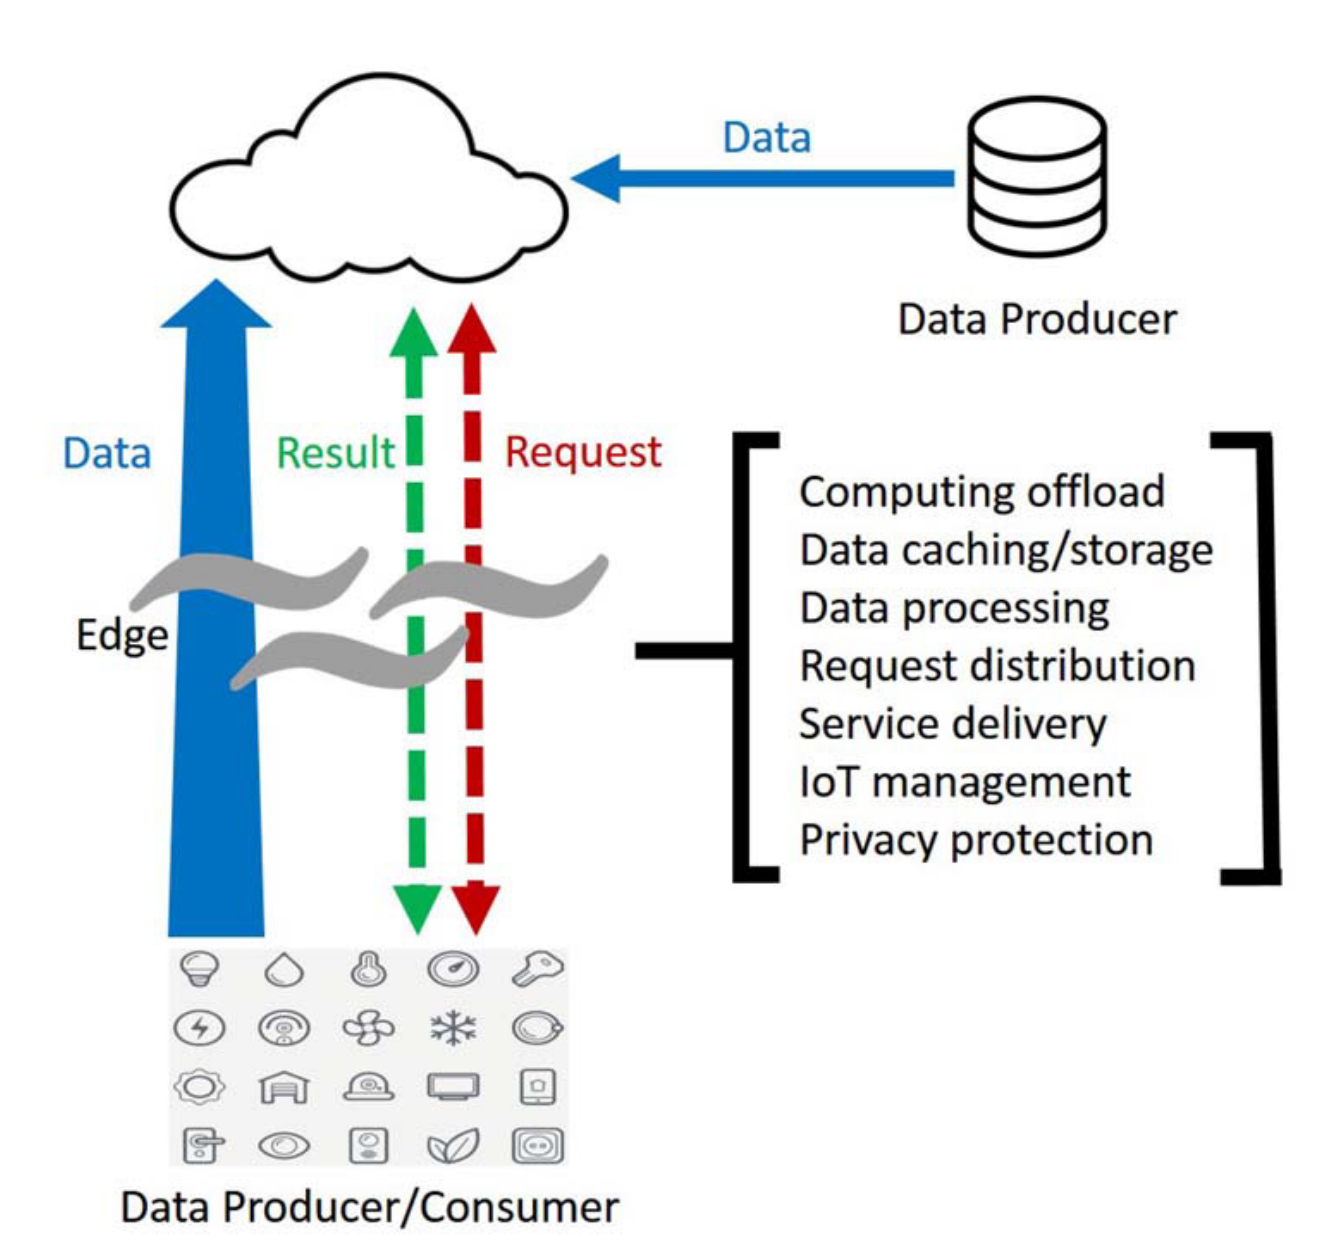
\includegraphics[width=0.6\textwidth]{figuras/edge-computing.png}
\caption{Paradigma de \emph{Edge Computing} \cite{Shi2016}.}
\label{edge-computing}
\end{figure}

\subsection{Computação em Névoa}

\citeonline{Dastjerdi2016} e \citeonline{IEEECommunicationsSociety2018}
mencionam que a enorme massa de dados gerados por ambientes IoT pode ser
processada pela nuvem, entretanto a latência produzida pela transferência desses
dados para a nuvem e o retorno do resultado não são tolerados por sistemas
críticos que sejam sensíveis a latência (monitoramento de saúde e resposta a
emergências). O autor ainda acrescenta que enviar tantos dados a \emph{cloud}
para processamento e armazenamento pode ser ineficiente e não escalável devido a
saturação de dados na rede. O \emph{edge computing} foi proposto para trazer o
processamento e armazenamento para os dispositivos de borda tentando solucionar
esses problemas, porém os dispositivos de borda não podem lidar com várias
aplicações IoT competindo pelos seus recursos limitados, o que poderia causar a
contenção dos recursos e aumento na latência do processamento
\cite{Dastjerdi2016}. Portanto, para solucionar estas questões de latência e
capacidade limitada dos dispositivos de borda, a computação em névoa foi proposta.

A computação em névoa (\emph{fog computing}) é um paradigma que distribui
as capacidades de computação, armazenamento e rede entre os nós próximos das fontes dados
e dos dispositivos finais, mas não necessariamente localizados na borda,
dando a esses nós características de uma nuvem
\cite{Bonomi2012,Dastjerdi2016,IEEECommunicationsSociety2018}.
Esse tipo de computação evita a sobrecarga dos dispositivos de borda.
\citeonline{Bonomi2012} e
\citeonline{Dastjerdi2016} veem o \emph{fog computing} como complementar da
\emph{edge computing}, podendo a computação em névoa aproveitar os recursos da
nuvem e da borda. \citeonline{IEEECommunicationsSociety2018} considera que a
principal diferença entre esses dois tipos de computação está no número de
camadas. Enquanto o \emph{edge computing} tem camadas menores, pois atua só nos
dispositivos de borda, o \emph{fog computing} tem mais camadas e um modelo
hierárquico, pois não atua só na camada de borda.

Segundo \citeonline{Bonomi2012} e \citeonline{Dastjerdi2016}, as principais
características da computação em névoa são:

\begin{itemize}

    \item \textbf{Mobilidade:} é essencial que as aplicações \emph{fog} sejam
    capazes de se comunicar com dispositivos móveis, por exemplo, utilizando
    protocolos que considerem a mobilidade dos nós;

    \item \textbf{Heterogeneidade:} os nós nesse tipo de paradigma possuem
    configurações e formatos diferentes e podem estar implantados em ambientes
    distintos;

    \item \textbf{Baixa Latência:} a computação em névoa foi proposta para
    atender aplicações que requeiram baixa latência (monitoramento de saúde,
    jogos, realidade aumentada, etc.);

    \item \textbf{Distribuição geográfica:} o \emph{fog computing} possui
    milhares de sensores e dispositivos distribuídos geograficamente e a
    consciência da localização deles (\emph{location awareness});

    \item \textbf{Alto número de nós:} seguindo os ambientes IoT, a computação
    em névoa pode ser composta por milhares de nós;

    \item \textbf{Interoperabilidade e federação:} os componentes da computação
    em névoa devem ser capazes de interoperar, e o serviços devem ser federados
    ao longo de diferentes domínios;

    \item \textbf{Uso de fluxo de dados e aplicações em tempo real:} a
    computação em névoa pode envolver aplicações que processam em lote, mas na
    maior parte das vezes envolve aplicações com requisito de processamento em
    tempo real, e para isso fazem o uso de fluxo de dados. Por exemplo, os
    sensores de um rede IoT escrevem a informação no fluxo de dados, a
    informação é processada, ações são inferidas e traduzidos em
    ações nos componentes atuadores.

\end{itemize}

Algumas aplicações para computação em névoa são: cidades inteligentes e
semáforos inteligentes que enviam sinais de alerta aos veículos e coordenam os
sinais verdes com outros semáforos através de sensores (veículos, pedestres,
ciclistas); na área de saúde para monitorar e prever situações de pacientes que
estão conectados a sensores; em prédios inteligentes que são dotados de sensores
de umidade, temperatura, qualidade do ar, ocupação, então a partir das
informações deles é possível alertar os ocupantes do prédio em algum caso de
emergência.

% \emph{Edge} é por vezes chamado de Computação em Névoa (\emph{Fog Computing})
% contudo \citeonline{IEEECommunicationsSociety2018} indica diferenças como exclusão do
% modelo \emph{cloud} e limitação a poucas camadas (por exemplo, somente os nós folha de uma rede)
% no modelo \emph{edge} em direto contraste com a inclusão de \emph{cloud} e hierarquias
% maiores. \emph{Fog} também atende gerenciamento da rede, armazenamento e controle.

% Fog works with the cloud, whereas edge is defined by the exclusion of cloud. Fog
% is hierarchical, where edge tends to be limited to a small number of layers. In
% additional to computation, fog also addresses networking, storage, control and
% acceleration. \cite{IEEECommunicationsSociety2018}

% Definição de Fog Computing
% o que é e como se relaciona com IoT e se diferencia das outras

% From our point of view, edge computing is interchangeable with fog computing [19], 
% but edge computing focus more toward the things side, while fog computing focus more 
% on the infrastructures ide.

% Esse modelo de computação distribuída desde os nós folha até o centro é motivado
% pela mudança do \emph{statu quo} do fluxo dos dados na internet: tradicionalmente
% os dados são produzidos pelos dispositivos de borda imediatamente enviados à 
% \emph{cloud} (produção, \emph{upstream}),
% que armazena e processa recursos derivados servido-os através de requisição-resposta
% (consumo, \emph{downstream}) a mais clientes.
% Com a ampliação da Internet das Coisas (\emph{Internet of Things}, IoT) e consequente
% ampliação sem precedentes do volume de dados gerados, mudando o relação de consumo
% e produção \cite{Shi2016}, arquiteturas tradicionais como \emph{cloud} podem não
% ser capazes de lidar com esses dados por falta de banda o que leva as
% propostas de distribuição vertical do processamento em \emph{fog} \cite{Bonomi2012, Dastjerdi2016}.

% Previous work such as micro datacenter [12], [13], cloudlet [14], and fog computing [15]
% [15] F. Bonomi, R. Milito, J. Zhu, and S. Addepalli,
% “Fog computing and its role in the Internet of things,” 
% in Proc. 1st Edition MCC Workshop Mobile Cloud Comput., Helsinki, Finland, 2012, pp. 13–16.

% Fog Computing: Helping the Internet of Things Realize Its Potential
% \cite{Dastjerdi2016}
% The Internet of Things (IoT) could enable
% innovations that enhance the quality of life, but it
% generates unprecedented amounts of data that
% precedented amounts of data that can be useful in many ways, par-
% are difficult for traditional systems, the cloud, and
% even edge computing to handle. Fog computing
% is designed to overcome these limitations.

\section{Mineração de Dados e Fluxo de Dados}

% Faria nem Silva definem ou citam data mining
% A data stream (DS) is a sequence of examples that arrive continuously. They are
% continuous, unbounded, flow at high speed and have a data distribution that
% may change over time \cite{Silva2013}. In DS scenarios, new concepts may
% appear and known concepts may disappear or evolve. \cite{Faria2016nd}

A Mineração de Dados é o processo de descoberta de padrões em conjuntos de dados
utilizando métodos derivados de aprendizagem de máquina, estatística e banco de
dados \cite{Gaber2005}. Um caso de mineração de dados é o \emph{Big Data} onde o
conjunto de dados não pode ser processado em um tempo viável devido a limitações
como memória ou armazenamento principal.

% Data stream mining is concerned with the extraction of knowledge from large
% amounts of continuously generated data in a non-stationary environment. Novelty
% detection (ND), the ability to identify new or unknown situations not
% experienced before, is an important task for learning systems, especially when
% data are acquired incrementally (Perner 2008). In data streams (DSs), where new
% concept can appear, disappear or evolve over time, this is an important issue to
% be addressed. ND in DSs makes it possible to recognize the novel concepts, which
% may indicate the appearance of a new concept, a change in known concepts or the
% presence of noise (Gama 2010).
% 
% Perner P (2008) Concepts for novelty detection and handling based on a case-based
% reasoning process scheme. Eng Appl Artif Intell 22:86–91
% 
% Gama J (2010) Knowledge discovery from data streams, vol 1, 1st edn. CRC press chapman hall, Atlanta

% dados massivamente e continuamente gerados e não persistentes. Fp

% \cite{Gaber2005} Cited by 1174
% Data mining is that interdisciplinary field of study that can extract models
% and patterns from large amounts of information stored in data repositories
% [30, 31, 34].
% 
% Recently, the data generation rates in some data sources become faster than ever
% before. This rapid generation of continuous streams of information has
% challenged our storage, computation and communication capabilities in computing
% systems. Systems, models and techniques have been proposed and developed over
% the past few years to address these challenges [5, 44]

Além da dimensão de armazenamento outra dimensão que afeta a maneira como dados
são modelados e manipulados é o tempo. Um Fluxo de Dados (\emph{Data Stream}) é
uma sequência de registros produzidos a uma taxa muito alta, associadas ao tempo
real, ilimitados, que excede recursos de armazenamento \cite{Gaber2005}.
Modelos de mineração de fluxo de dados atendem a esses desafios utilizando
restrições como apenas uma leitura do conjunto de dados e complexidade
de processamento menor que linear \cite{Gama2007, Gaber2005}.

\nota{Não faz sentido considerar como fluxo somente se a taxa for muito alta.
Precisa rever isto.}

\nota{O que é complexidade menor que linear em fluxos? }

% \nota{falta abordar processamento paralelo e distribuído}

As características de fluxos de dados e mineração de dados e os requisitos de
seu processamento regularmente superam as capacidades computacionais de um único
nó computacional convencional, portanto a distribuição dos requisitos em
múltiplos nós computacionais em um sistema distribuído é igualmente necessária
\cite{Gaber2005}.

Computação distribuída é a área da ciência da computação que estuda sistemas
onde os componentes são localizados em diferentes computadores (nós) que
comunicam-se apenas por troca de mensagens e, para que o objetivo do sistema
seja atingido, a cooperação entre os nós é necessária.
Outras propriedades de um sistema distribuído são a concorrência entre nós e
falhas em partes independentes \cite{TanenbaumSteen2018}.

% - quem são, o que consomem
% (\citeonline{Viegas2019} \emph{apud} \citeonline{Gaber2005}) Mining data streams: A Review.
% {Gaber2005} apud [47] {Park2002distributed}
% [47] B. Park and H. Kargupta. Distributed Data Mining: Algorithms, Systems, and
% Applications. To be published in the Data Mining Handbook. Editor: Nong Ye.
% 2002.]

% A data stream is a sequence of unbounded, real-time data records that are
% characterized by the very high data rate, which stresses our computational
% resources, and can be read only once by processing applications [13,8,1,9]
 
% [1] B. Babcock, S. Babu, M. Datar, R. Motwani, J. Widom, Models and issues in
% data stream systems. In: Proceedings of Principles of Database Systems
% (PODS’02), pp. 1–16, 2002. \cite{Babcock2002}

% [2] G. Boone, Reality mining: browsing reality with sensor networks.
% In: Sensors Online, vol. 21, 2004.

% [3] V. Cantoni, L. Lombardi, P. Lombardi, Challenges for data mining in
% distributed sensor networks. ICPR (1) 1000–1007, 2006

% [8] M.M. Gaber, A. Zaslavsky, S. Krishnaswamy, Mining data streams: a review.
% ACMSIGMOD Record, 34(2):18–26, 2005.
% 
% [9] M. Garofalakis, J. Gehrke, R. Rastogi, Querying and mining data streams:
% you only get one look a tutorial. In: Proceedings of the 2002 ACM SIGMOD
% International Conference on Management of Data, June 03–06, Madison, Wisconsin,
% 2002.
% 
% [13] S. Muthukrishnan, Data streams: algorithms and applications. In:
% Proceedings of the Four- teenth Annual ACM-SIAM Symposium on Discrete
% Algorithms, 2003.

% Mineração de Fluxo de Dados é análogo à mineração de
% dados e \emph{big data} com a restrição temporal onde um registro é unicamente 
% associado um tempo, dessa forma além de não ser possível manipular o conjunto
% de dados em memória, não é possível recuperar dados fora do intervalo de tempo associado
% a eles.

% ----- wikipedia ------
% 
% Data mining is the process of discovering patterns in large data sets involving
% methods at the intersection of machine learning, statistics, and database
% systems.[1] Data mining is an interdisciplinary subfield of computer science and
% statistics with an overall goal to extract information (with intelligent
% methods) from a data set and transform the information into a comprehensible
% structure for further use.[1][2][3][4] Data mining is the analysis step of the
% "knowledge discovery in databases" process or KDD.[5] Aside from the raw
% analysis step, it also involves database and data management aspects, data
% pre-processing, model and inference considerations, interestingness metrics,
% complexity considerations, post-processing of discovered structures,
% visualization, and online updating.[1]
% 
% [1] "Data Mining Curriculum". ACM SIGKDD. 2006-04-30. Retrieved 2014-01-27.
% [2] Clifton, Christopher (2010). "Encyclopædia Britannica: Definition of Data Mining". Retrieved 2010-12-09.
% [3] Hastie, Trevor; Tibshirani, Robert; Friedman, Jerome (2009).
% "The Elements of Statistical Learning: Data Mining, Inference, and Prediction".
% Archived from the original on 2009-11-10. Retrieved 2012-08-07.
% [4] Han, Kamber, Pei, Jaiwei, Micheline, Jian (June 9, 2011).
% Data Mining: Concepts and Techniques (3rd ed.). Morgan Kaufmann. ISBN 978-0-12-381479-1.
% [5] Fayyad, Usama; Piatetsky-Shapiro, Gregory; Smyth, Padhraic (1996).
% "From Data Mining to Knowledge Discovery in Databases" (PDF). Retrieved 17 December 2008.


\section{Arquiteturas e Plataformas de Processamento de Fluxos}

% - arq lambda, kappa, (vide guilherme)

% Existem diversas maneiras de organizar o caminho das informações em um
% aplicativo de processamento de fluxo de dados. Algumas propostas sao amplamente
% conhecidas como as arquiteturas Lambda (MARZ; WARREN, 2015) e Kappa (KREPS,
% 2014), as quais s˜ao genéricas e focadas no processamento de fluxo.

% A arquitetura Lambda (MARZ; WARREN, 2015) mescla o processamento do fluxos de
% dados com o processamento em lotes. O objetivo dessa mistura é obter, ao mesmo
% tempo, a capacidade de fazer análises em tempo real, e, ao mesmo tempo,
% fazê-las com maior qualidade. Seu processamento é dividido em duas camadas,
% uma camada de processamento online que fornece resultados aproximados com baixa
% latência e uma camada de processamento offline que usa os dados históricos
% disponíveis e fornece resultados mais precisos, embora com maior sobrecarga e
% latência. Além das duas camadas de processamento, a Arquitetura Lambda possui
% uma camada de serviço, que combina dados de ambas as camadas de processamento e
% apresenta ao usuário.

% A arquitetura Kappa, por outro lado, possui apenas as camadas de processamento e
% serviço de fluxo. Seu objetivo é o processamento em tempo real, portanto
% possui a menor quantidade possível de sobrecarga e latência. Sendo assim, é
% natural que esta seja uma arquitetura muito simples e que possua apenas os
% módulos essenciais para um sistema de processamento de fluxo. A arquitetura
% Kappa possui apenas um módulo de processamento on-line que opera através do
% fluxo de dados e fornece informações.

% MARZ, N.; WARREN, J. Big Data: Principles and Best Practices of Scalable
% Realtime Data Systems. 1st. ed. Greenwich, CT, USA: Manning Publications Co.,
% 2015. ISBN 1617290343, 9781617290343. \cite{marz2015big}

% KREPS, J. Questioning the Lambda Architecture. 2014. Disponível em:
% https://www.oreilly.com/ideas/questioning-the-lambda-architecture

\nota{Os conceitos ficaram um tanto misturados nesta seção. Acho que ficaria
melhor se dividisse em 2 ou 3 seções, por exemplo: uma seção sobre processamento
em batch ou {\it offline} como Mapreduce/Hadoop, ou o Spark originalmente; uma
segunda seção poderia falar somente de plataformas de processamento de fluxos;
terceira poderia falar sobre as arquiteturas (lambda, kappa) que combinam de
certa forma as plataformas offline e de fluxos. Acho que kafka poderia aparecer
dentro dessa terceira seção.}


Tradicionalmente, aplicações foram construídas com um sistema gerenciador de
banco de dados (SGBD) relacional ou não-relacional associado. Essa arquitetura,
nomeada de arquitetura totalmente incremental por \citeonline{marz2015big},
foi evoluída e simplificada iterativamente durante décadas de uso, porém ela não
é adequada para sistemas em tempo real, como os sistema de fluxo de dados.


\nota{Eu nem citaria SGBD, isso foi novidade há uns 30 ou 40 anos. Mapreduce já
tem praticamente 20 anos ... }

\newcommand{\lambdaa}{\xspace\emph{Lambda}\xspace}
\newcommand{\kappaa}{\xspace\emph{Kappa}\xspace}

O volume e velocidade de dados em um \emph{Data Stream} leva a necessidade de
distribuir o processamento acrescentando poder computacional a cada nó
adicionado, porém desafios como comunicação eficiente e sincronização de estado
entre os nós assim como tolerância a falhas aumentam a complexidade de
construção de um sistema distribuído em relação a um sistema tradicional.
Para mitigar esses problemas foram propostas arquiteturas de processamento de fluxo
de dados distribuído, como arquitetura \lambdaa \cite{marz2015big} e \kappaa \cite{Kreps2014}, além de
diversas plataformas tanto de \emph{Big Data} com características de tempo real
como especializadas em fluxo de dados.

\nota{Tem referências para Lambda e Kappa? }

A arquitetura \lambdaa divide o processamento em três camadas: lotes, serviço
e velocidade. A camada de lotes atua sobre o conjunto mestre em modo de leitura
sequencial, armazenando-o em sistema de arquivos distribuído e pré-processando
várias visões sobre esse conjunto mestre. Essas visões (armazenadas num SGBD
tradicional) são consumidas pela camada de serviço, que portanto tem acesso
regular (leitura aleatória).
No entanto, as garantias oferecidas pela camada de
lotes (escalabilidade, consistência, tolerância a falhas) não atendem os requisitos
de latência em um sistema em tempo real, portanto a camada de velocidade
complementa os dados das visões com dados diretamente do conjunto mestre em
tempo real diretamente para a camada de serviço \cite{marz2015big}.

A Figura \ref{fig:lambda} ilustra uma implementação da arquitetura \lambdaa
onde a \emph{Apache Kafka}, \emph{Apache Storm}, \emph{Apache Hadoop}
implementam o conjunto mestre, camada de velocidade e camada de lotes
respectivamente.

\begin{figure}[ht]
\centering
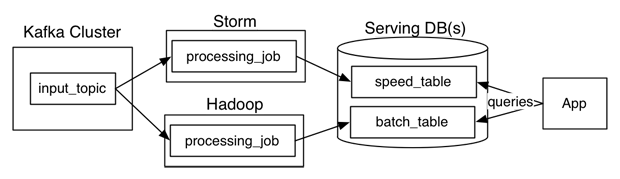
\includegraphics[width=0.6\textwidth]{figuras/lambda.png}
\caption{Arquitetura \lambdaa com detalhes práticos \cite{Kreps2014}.}
\label{fig:lambda}
\end{figure}

Em contraposição à arquitetura \lambdaa, observações práticas de 
\citeonline{Kreps2014} mostram que o sistema de fila de mensagens
(no exemplo \emph{Apache Kafka}) já traz as garantias de
escalabilidade, consistência, tolerância a falhas, replicação e armazenamento de longo prazo.
Com isso, \citeonline{Kreps2014} propõe que as camadas de lotes e velocidade sejam
unificadas em uma camada de processamento de fluxo, cujos resultados sejam entregues
continuamente para a camada de serviço através de um SGBD, definindo assim a arquitetura \kappaa.
Essa proposta simplifica a aplicação de três implementações para duas eliminando a
repetição de tarefas executadas pelas camadas de lotes e velocidade que
produziam o mesmo resultado.

% A arquitetura \kappaa limita-se ao processamento de \emph{Stream} apenas
% \emph{on-line} destila outras observações quanto a complexidade temporal do
% sistema completo de que se uma aplicação não processa os dados em tempo menor
% que linear, dados serão perdidos ou a complexidade espacial são será satisfeita,
% em resumo, a aplicação sempre deve ser mais rápida que o \emph{Stream}
% \cite{marz2015big}.

% - MapReduce, Hadoop, Spark, Storm
% Breve descrição do MapReduce e Hadoop
% O que são e para que servem essas ferramentas

Em sincronia com os desenvolvimentos em arquiteturas de processamento de fluxo de dados,
durante as últimas duas décadas foram construídas diversas plataformas de
processamento para \emph{Big Data} e \emph{Data Streams}.
% A seguir descrevemos algumas das mais notáveis (?)

\emph{MapReduce} é a primeira plataforma de processamento de conjuntos massivos
de dados que atingiu uso generalizado.
Nessa implementação uma biblioteca
gerencia a distribuição, paralelização, tolerância a falhas e balanceamento de
carga.
Ao usuário da biblioteca resta implementar duas funções:
\emph{Map} que recebe um par ordenado
$(chave, valor)$ e emite um conjunto de pares intermediários na mesma estrutura;
\emph{Reduce} recebe uma chave e um conjunto de valores gerado pelo agrupamento
de pares com essa mesma chave \cite{Dean2004}.

Em prática, um \emph{cluster MapReduce} tem centenas de processadores e o conjunto de dados é
armazenado em um sistema de arquivos distribuído que é lido pela plataforma com
programas escritos por usuários sendo executados sob supervisão de um nó mestre.
Essa implementação tem esquema geral de processamento em lotes que não atende o
requisito de baixa latência.
\nobreakdash \emph{MapReduce} é uma das principais influências na criação da arquitetura
\lambdaa \cite{marz2015big}.

\emph{Apache Hadoop} é uma coleção de ferramentas incluindo: \emph{Hadoop
Distributed File System} (HDFS) um sistema de arquivos distribuído, \emph{Hadoop
YARN} um gerenciador de recursos em cluster e escalonador de trabalhos e,
\emph{Hadoop MapReduce} um sistema baseado em \emph{YARN} implementando o modelo
\emph{MapReduce} \cite{ApacheHadoop2020}.

% Breve descrição do Apache Spark

% Spark is an open-source cluster computing framework with a large global user base.
% It is written in Scala, Java, R, and Python and gives programmers an Application Programming Interface (API)
% built on a fault tolerant, read-only multiset of distributed data items.
% In two years since its initial release (May 2014), it has seen wide acceptability for real-time,
% in-memory, advanced analytics — owing to its speed, ease of use, and the ability to handle
%  sophisticated analytical requirement
% https://dzone.com/articles/streaming-in-spark-flink-and-kafka-1

% Apache Spark is an open-source distributed general-purpose cluster-computing
% framework. Spark provides an interface for programming entire clusters with
% implicit data parallelism and fault tolerance. Originally developed at the
% University of California, Berkeley's AMPLab, the Spark codebase was later
% donated to the Apache Software Foundation, which has maintained it since.

% Apache Spark is a fast and general-purpose cluster computing system. It provides
% high-level APIs in Java, Scala, Python and R, and an optimized engine that
% supports general execution graphs. It also supports a rich set of higher-level
% tools including Spark SQL for SQL and structured data processing, MLlib for
% machine learning, GraphX for graph processing, and Spark Streaming.

\emph{Apache Spark}, analogamente ao \emph{Hadoop}, é um \emph{framework} para
construção de sistemas de computação distribuída em \emph{cluster} com garantias
de tolerância a falhas. No entanto, o modelo de processamento diverge
significativamente do tradicional \emph{MapReduce} utilizando em lugar do HDFS
um multiconjunto de apenas leitura distribuído (\emph{Resilient Distributed Dataset}
- RDD) com um escalonador de trabalhos representados por grafos acíclicos
direcionados (\emph{directed acyclic graph} - DAG), otimizador de consultas e
motor de execução \cite{ApacheSpark2020}.

% MapReduce programs read input data from disk, map a function across the data,
% reduce the results of the map, and store reduction results on disk.
% Spark's RDDs function as a working set for distributed programs that offers a
% (deliberately) restricted form of distributed shared memory.[8]

Enquanto programas \emph{MapReduce} fazem sua entrada de dados por leitura de um
disco, executam a função \emph{Map} em todos os items, agrupam, executam
\emph{Reduce} e armazenam o resultado em disco novamente, o RDD opera com um
conjunto de trabalho distribuído em formato de memória compartilhada com
restrições. Esse conjunto de trabalho distribuído facilita programas iterativos
que são típicos de análise, mineração de dados e aprendizado de máquina.

Uma das extensões do \emph{Apache Spark} é o \emph{Spark Streaming} que é um
sistema de processamento de fluxo de dados escalável e tolerante a falhas
\cite{zaharia2016,sparkStreaming2016}.
O \emph{Spark Streaming} implementa o processamento incremental de fluxo de
dados usando o modelo de fluxos discretizados em que divide-se os dados de entrada
em micro-lotes (ex: a cada 100 milissegundos) e combina-se regularmente com o
estado nos RDDs para produzir novos resultados \cite{zaharia2016}.
Essa estratégia traz benefícios sobre os sistemas de fluxos de dados distribuídos
tradicionais, pois permite a consistência e recuperação de falhas rapidamente
devido a linhagem de RDD (\emph{RDD lineage}) e combinação do fluxo de dados com
consultas em lotes e interativas \cite{sparkStreaming2016,Lopez2018}.

O \emph{Apache Storm} é um sistema de computação tolerante a falhas em tempo
real que facilita o processamento de fluxo de dados
\cite{ApacheStorm2020,Lopez2018}.
Ao invés de executar trabalhos (\emph{jobs}) como algumas ferramentas citadas
anteriormente, o \emph{Apache Storm} executa topologias.
Os \emph{jobs} eventualmente finalizam, e as topologias executam continuamente até
serem finalizadas por comandos.
Uma topologia constitui de processos \emph{workers} sendo executados
em um \emph{cluster} de nós que são gerenciados pelo nó mestre que além de
coordenar e distribuir execução, monitora falhas.
Uma topologia pode ser representada por um grafo de computação direcionado
acíclico (DAG).

Além de topologias e nós mestre, outros componentes do funcionamento dessa
ferramenta são os \emph{spouts} e os \emph{bolts}.
O \emph{spout} representa uma fonte de dado da ferramenta, sendo um ponto de
entrada que lê os dados de fontes externas, converte-os para um fluxo de dados e
emite-os para dentro da topologia.
Os \emph{bolts} recebem os dados de um \emph{spout} e processam esses dados
(filtragem, funções de agregação e união, etc.).

Cada processo \emph{worker} no \emph{Storm} é uma instância de Java Virtual Machine (JVM)
e executa um conjunto de tarefas para uma topologia processando um ou mais
executores.
Um executor é uma \emph{thread} gerada por um processo \emph{worker}.
Cada executor pode processar uma ou mais tarefas para um mesmo componente
(\emph{spout} ou \emph{bolt}).
O número de processos \emph{workers}, executores e tarefas (para os
\emph{spouts} e \emph{bolts}) que são passados como parâmetro (\emph{parallelism
hint}) definem o ``paralelismo'' do \emph{Storm}. A principal característica desse
paralelismo é que ele pode ser alterado em tempo de execução da topologia.

% Em relação a distribuição num \emph{cluster} do \emph{Apache Storm}, uma máquina
% pode rodar bolsinha um ou mais processos \emph{workers} de uma ou mais topologias.

% Foi desenvolvido no AMPLab da Universidade da Califórnia[2] e posteriormente
% doado para a Apache Software Foundation[3] que o mantém desde então.

% Spark provê uma interface para programação de clusters com paralelismo e
% tolerância a falhas.

% Apache Spark \cite{Zaharia} é um 
% (execução em computadores não confiáveis) utilizando como premissas: paralelização
% e localidade de dados, como 

% The lambda and the Kappa
% 12. M. Zaharia et al., “Discretized Streams: Fault-Tolerant
% Streaming Computa- tion at Scale,” Proc. 24th ACM Symp

% api em Python (dataframe de pandas)
% ------------------------------------------------------------------------------------------------------
\section{Apache Flink}

O \emph{Apache Flink} é uma plataforma de processamento distribuído para
computação \emph{stateful} sobre fluxo de dados limitados (tem um início e um
fim) e ilimitados (não tem um fim definido) \cite{ApacheFlink2020}.
Essa plataforma segue um paradigma que abrange o processamento de fluxos de
dados contínuos e o processamento em lote \cite{Carbone2015,Lopez2018}.
O \emph{Apache Flink} pode ser integrado a vários gerenciadores de \emph{cluster}
comuns, como \emph{Hadoop Yarn}, \emph{Apache Mesos}, e \emph{Kubernetes}, mas também pode ser
configurado para ser executado como um \emph{cluster stand-alone}.
Já o acesso programático a essa plataforma pode ser feito através das linguagens
Java, Scala ou Python.

\subsection{Arquitetura}

Quando o \emph{Flink} é inicializado, o \emph{Job Manager} e um ou mais
\emph{Task Manager} são criados.
Quando um código de programa é submetido, o cliente transforma-o em um grafo
acíclico direcionado - \emph{data flow} - e submete-o ao \emph{Job Manager},
como pode ser observado na Figura Figura \ref{fig:processo-flink}.
Segundo \citeonline{Carbone2015}, essa fase de transformação examina o esquema
dos dados trocados entre os operadores e cria serializadores e
outros códigos para otimização da futura execução.
O \emph{Job Manager} coordena toda execução distribuída do grafo \emph{data
flow}. Ele rastreia o estado e o progresso de cada fluxo, agenda novos
operadores e coordena os \emph{checkpoints} e recuperação.
Para alta disponibilidade, o \emph{Job Manager} persiste um conjunto mínimo de
metadados em cada \emph{checkpoint} para um armazenamento tolerante a falhas, de
modo que esse gerenciador possa recuperar a execução do grafo a partir desse
ponto.
O processamento de dados ocorre no \emph{Task Manager} que executa um ou mais
operadores que produzem fluxos de dados, e reportam seus estados ao \emph{Job
Manager}.

\begin{figure}[hbt]
\centering
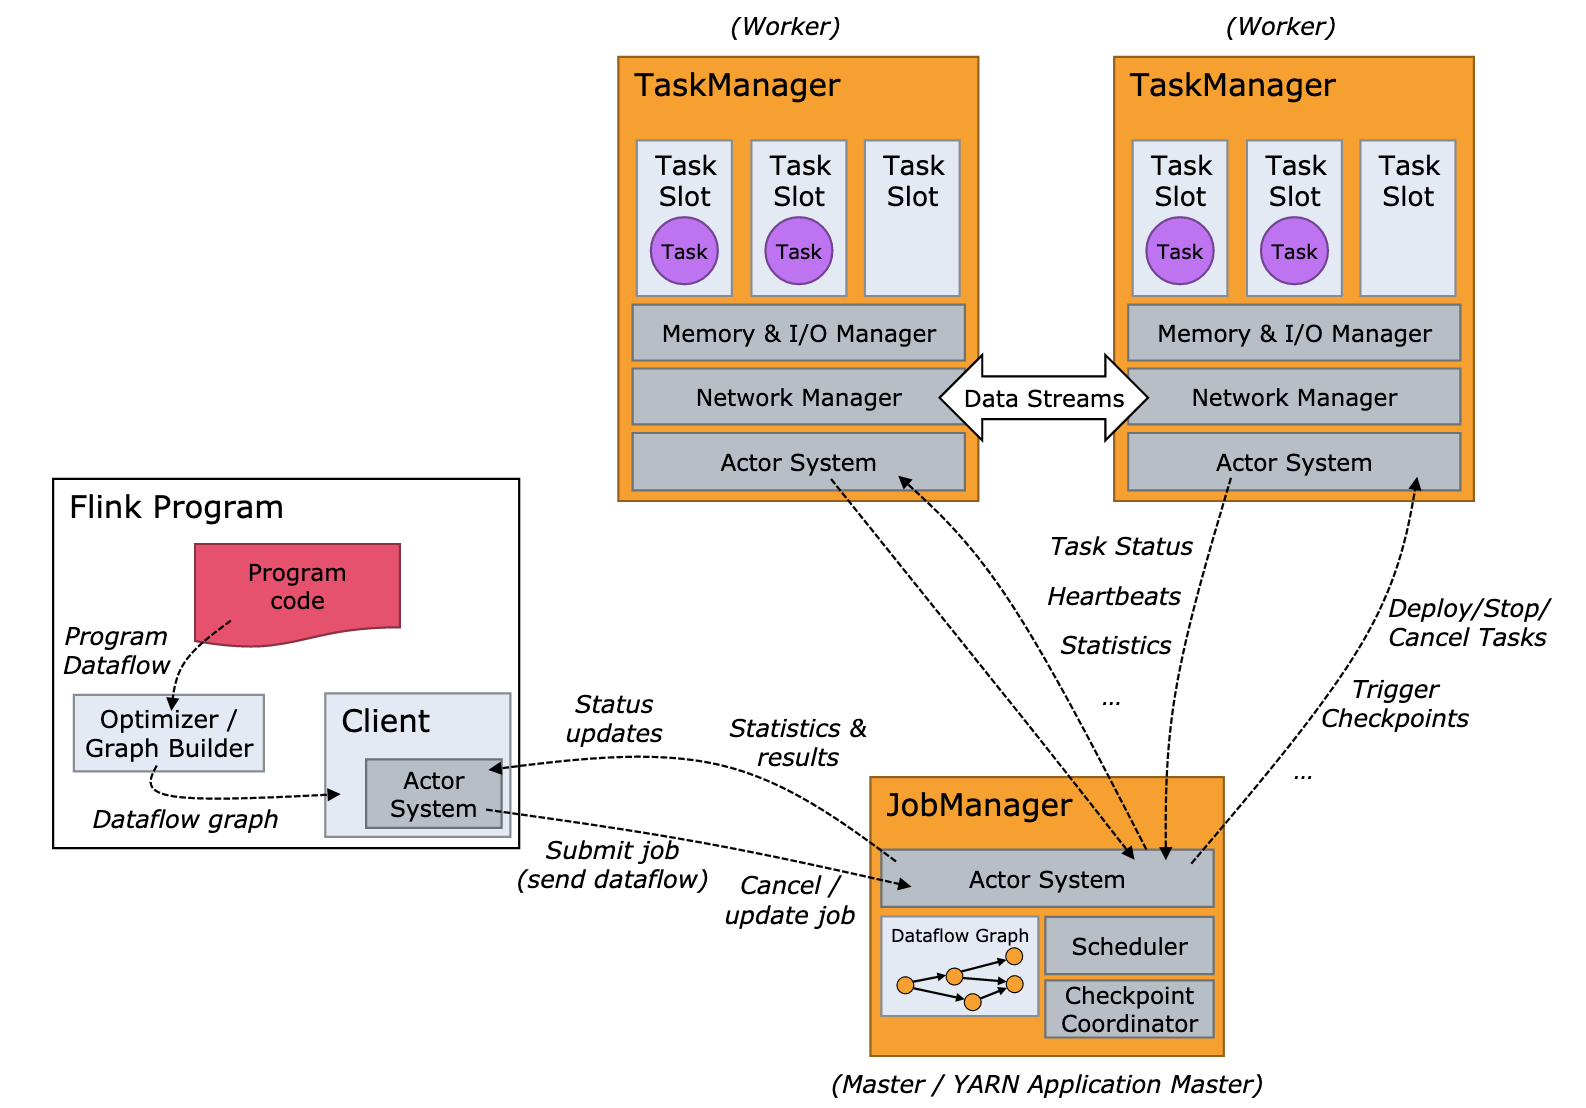
\includegraphics[width=0.8\textwidth]{figuras/processo-flink.png}
\caption{Processo do \emph{Apache Flink} \cite{ApacheFlink2020}}
\label{fig:processo-flink}
\end{figure}

A pilha de componentes de software do \emph{Apache Flink} é composta pelas
seguintes camadas da Figura \ref{fig:software-flink}.
A camada \emph{core} é vista como um mecanismo de processamento e execução de
fluxo de dados, enxergando o processamento em lote como um caso especial
\cite{Lopez2018,Carbone2015}.
A camada de APIs é composta pelo \emph{DataStream API} que processa dados
infinitos ou fluxos de dados e pelo \emph{DataSet API} que processa dados
finitos ou dados em lote.
Junto ao \emph{core}, essas APIs montam planos de execução otimizados para cada
tipo de conjuntos de dados, gerando programas executáveis pelo \emph{core}.
Na camada de bibliotecas (\emph{libraries}), há bibliotecas específicas para
cada domínio que geram programas API \emph{Data Stream API} ou \emph{DataSet
API}.
Essas bibliotecas são: \emph{FlinkML} para aprendizado de máquina, \emph{Gelly}
para processamento de grafos, \emph{Table} para domínios relacionais (SQL), e
CEP (\emph{Complex Event Processing}) para processamento de eventos.

\begin{figure}[ht]
\centering
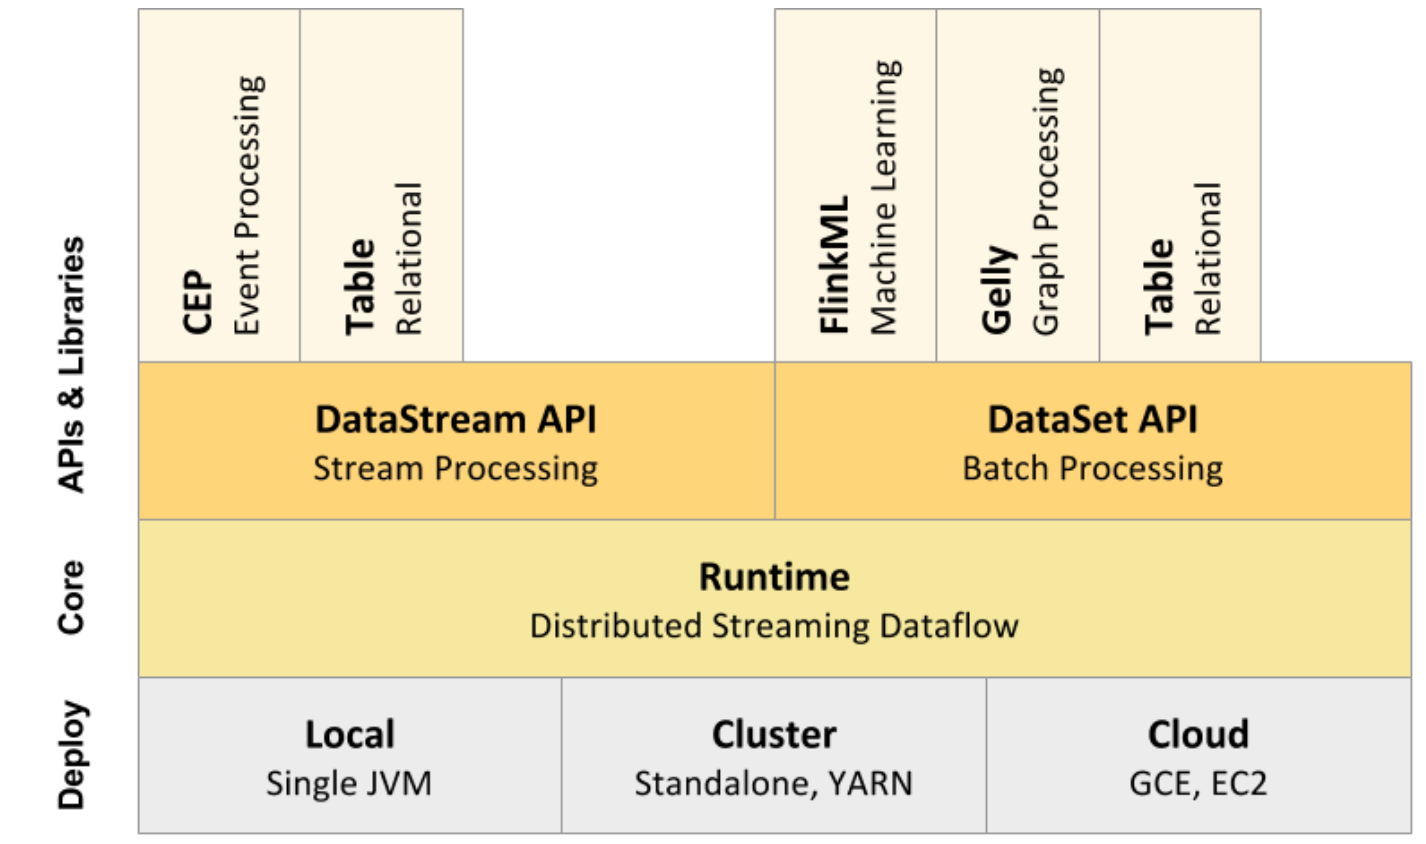
\includegraphics[width=0.7\textwidth]{figuras/software-flink.png}
\caption{Componentes de software do \emph{Apache Flink} \cite{Carbone2015}.}
\label{fig:software-flink}
\end{figure}

\subsection{\emph{Data flow} e \emph{data streams}}

Os \emph{data streams} ou fluxo de dados e as transformações são as principais
abstrações do \emph{Apache Flink} \cite{Lopez2018,ApacheFlink2020}.
Esse fluxo de dados é definido como um fluxo de registros.
Já as transformações são operações (\emph{map, filtering, reduction, join},
etc.) aplicadas de forma incremental nos \emph{data streams}, gerando um novo
fluxo de dados.
Cada uma dessas transformações pode ser paralelizada por um parâmetro de
paralelismo \cite{Lopez2018}.

Um programa \emph{Flink} é mapeado para um grafo acíclico direcionado \emph{data
flow} utilizado pelo \emph{Job Manager} \cite{Carbone2015}.
Esse grafo é composto por operadores de transformação e fluxo de dados
\cite{ApacheFlink2020}.
Para facilitar o paralelismo desse grafo de execução, os operadores que agem
sobres os fluxos de dados podem ser divididos em sub-tarefas que são executadas
pelos \emph{slots} dos \emph{Task Manager}, e os fluxos de dados podem ser
particionados entre os operadores consumidores e produtores.

Cada \emph{data flow} dos programas do \emph{Apache Flink} iniciam com uma fonte
de dados e terminam com um \emph{sink} que escreve os dados de saída em algum
sistema de armazenamento suportado, como: \emph{Apache Kafka, Amazon Kinesis Streams,
Hadoop Filesystem, Apache Cassandra} \cite{ApacheFlink2020}.
Na Figura \ref{fig:dataflow-flink}, pode-se observar um exemplo de programa
\emph{Apache Flink} escrito em Java e seu grafo de execução.
Nesse exemplo, define-se como fonte de dados o \emph{Apache Kafka}.
Em seguida, aplica-se uma transformação \emph{map}, e depois outra transformação
de agrupamento por um dos atributos dos dados e por uma janela de 10 segundos.
Por fim, o resultado é passado para um \emph{sink}.

\begin{figure}[ht]
\centering
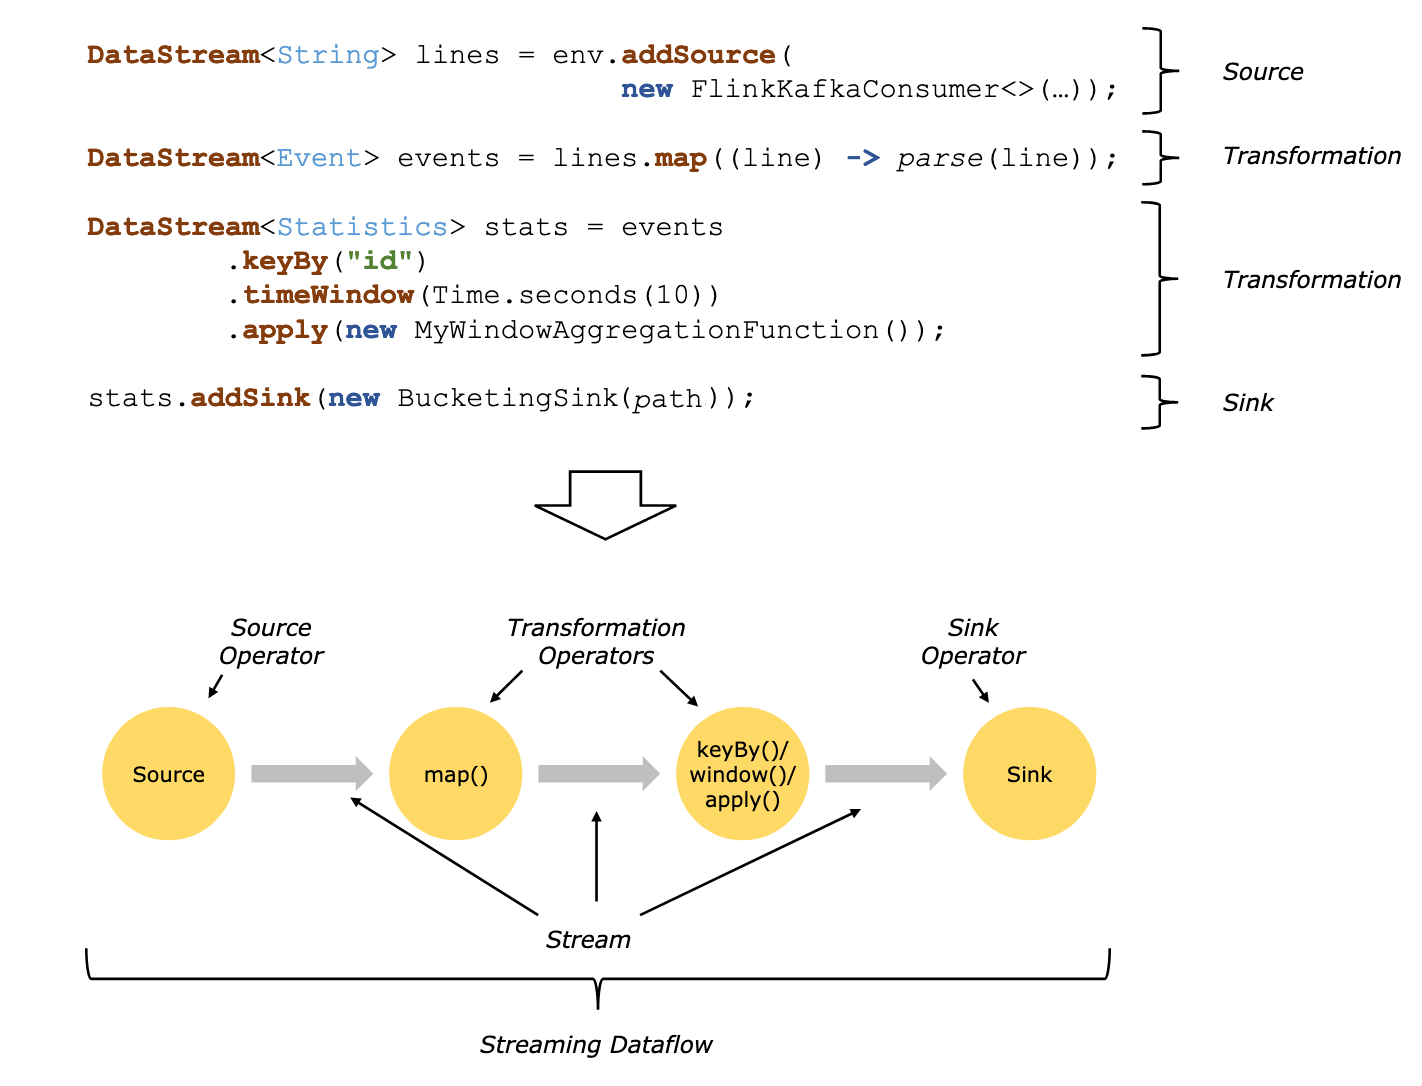
\includegraphics[width=0.85\textwidth]{figuras/dataflow-code-flink.png}
\caption{Exemplo de código e \emph{data flow} do \emph{Apache Flink} \cite{ApacheFlink2020}}
\label{fig:dataflow-flink}
\end{figure}

\subsection{Tolerância a falhas}

O \emph{Apache Flink} implementa a tolerância a falhas combinando repetição e
\emph{checkpoint} dos fluxos \cite{Carbone2015,ApacheFlink2020}.
Um \emph{checkpoint} está relacionado com pontos específicos dos fluxos de
entrada, juntamente com o estado dos operadores.
Um fluxo de dados pode ser retornado a partir de um \emph{checkpoint}, mantendo
a consistência de ``exatamente uma vez'' (não há dados duplicados e nem dados que
não sejam processados), e restaurando o estado dos operadores e eventos naquele
momento.
Portanto, as falhas são tratadas de forma transparente e não afetam a exatidão
da execução de um programa \emph{Flink} \cite{ApacheFlink2020}.

O algoritmo de \emph{checkpoint} assíncrono e incremental garante um impacto
mínimo em latência no processamento \cite{Carbone2015}.
Além disso, para reduzir o tempo de recuperação, o \emph{Apache Flink} tira um
\emph{snapshot} do estado dos operadores, incluindo a posição atual dos fluxos
de entrada em intervalos regulares.

% \subsection{Operações com Estado}

O \emph{Apache Flink} realiza computações com estado (\emph{stateful}) que guardam
eventos ou resultados intermediários para acessá-los posteriormente,
contribuindo para planos de execução, mecanismo de recuperação de falhas e
lembrar de eventos passados para agregar dados \cite{ApacheFlink2020, Carbone2015}.

% \subsection{Processamento em lotes}

O \emph{Apache Flink} considera o processamento em lotes como um caso especial
de fluxo de dados, que nesse caso é limitado em número de elementos.
Para esse tipo de dados, há estrutura de dados e algoritmos específicos, como o
\emph{DataSet API} e operações próprias (agregações, uniões, interações)
\cite{Carbone2015}.

Para o processamento em lote, não há o mecanismo de \emph{checkpoint} como há
para o fluxo de dados.
No lugar, a recuperação é feita repetindo completamente o fluxo ou repetindo as
últimas partições perdidas do fluxo intermediário materializado.



% \nota{Descrever o flink, diferenças entre as outras plataformas e dar exemplos de código}
% Breve descrição do Flink (como esse vai ser usado, precisa explicar um pouco melhor - 2 paginas pelo menos):\\
% - arquitetura\\
% - modelo de programacao\\
% - 1 pequeno exemplo de codigo explicando


% These stream applications are characterized by an unbounded sequence of
% events, or tuples, that arrive continuously [4]. \cite{Stonebraker2005}

% A number of requirements must be met on distributed stream processing
% platforms, \citeonline{Stonebraker2005} Stonebraker et al. highlight the most
% important [4].


% the difficulties in anonymizing and extracting knowledge from
% anonymized data, and discuss the main datasets available [6].
% Among the datasets for security research, the most commonly
% used is KDD [10], whose characterization was performed by
% Tavallaee et al. [15]. \cite{Lopez2017}

% \cite{Lopez2017}
% In this paper, we analyze and characterize the traffic of a broadband Internet
% access network by differentiating normal from anomalous traffic, that is marked
% as threat by an IDS. We collected real and anonymized data from a major
% telecommu- nications operator ^1. The dataset is created by capturing 5 TB of
% access data of 373 residential broadband users in the city of Rio de Janeiro,
% Brazil. The dataset contains legitimate traffic, attacks and other security
% threats
% ^1 Anonymized data can be consulted through email contact with authors.

% [4] STONEBRAKER, M., C¸ ETINTEMEL, U., ZDONIK, S. “The 8 requirements of
% real-time stream processing”, ACM SIGMOD Record, v. 34, n. 4, pp. 42–
% 47, 12 2005. ISSN: 01635808. doi: 10.1145/1107499.1107504.
% \cite{Stonebraker2005}
% [80] ANDREONI LOPEZ, M., LOBATO, A. G. P., MATTOS, D. M. F., et al. “Um
% Algoritmo Não Supervisionado e Rápido para Seleção de Caracterı́sticas
% em Classificação de Tráfego”. In: XXXV SBRC’2017, Belém- Pará, PA,,
% 2017.
% [81] ANDREONI LOPEZ, M., LOBATO, A. G. P., DUARTE, O. C. M. B., et al.
% “An evaluation of a virtual network function for real-time threat detection
% using stream processing”. In: IEEE Fourth International Conference on
% Mobile and Secure Services (MobiSecServ), pp. 1–5, 2018. doi: 10.1109/
% MOBISECSERV.2018.8311440.
% [82] CHENG, Z., CAVERLEE, J., LEE, K. “You Are Where You Tweet: A Content-
% based Approach to Geo-locating Twitter Users”. In: Proceedings of the
% 19th ACM International Conference on Information and Knowledge Man-
% agement, CIKM ’10, pp. 759–768. ACM, 2010. ISBN: 978-1-4503-0099-5.
% [83] LOBATO, A. G. P., ANDREONI LOPEZ, M., DUARTE, O. C. M. B. “Um
% Sistema Acurado de Detecção de Ameaças em Tempo Real por Processa-
% mento de Fluxos”. In: SBRC’2016, pp. 572–585, Salvador, Bahia, 2016.


% \{Messa queueing systems - Sistemas de filas de mensagens}
% O que são, para que servem e citar alguns exemplos
% \{Kafka}
% 1 pag

% Apache Flink % Apache Flink is an open-source platform for distributed stream
% and batch data processing. Flink’s core is a streaming data flow engine that
% provides data distribution, communication, and fault tolerance for distributed
% computations over data streams. Flink also builds batch processing on top of the
% streaming engine, overlaying native iteration support, managed memory, and
% program optimization.

% Advantages of Flink:

% Flink streaming processes data streams as true streams, i.e. data elements are
% immediately “pipelined” through a streaming program as soon as they arrive. This
% allows performing flexible window operations on streams.

% Better memory management: Explicit memory management gets rid of the occasional spikes found in Spark framework.

% Speed: It manages faster speeds by allowing iterative processing to take place
% on the same node rather than having the cluster run them independently. Its
% performance can be further tuned by tweaking it to re-process only that part of
% data that has changed rather than the entire set. It offers up to a five-fold
% boost in speed when compared to the standard processing algorithm.

% Apache Spark is considered a replacement for the batch-oriented Hadoop system.
% But it includes a component called Apache Spark Streaming, as well. Contrast
% this with Apache Flink, which is a Big Data processing tool and it is known to
% process big data quickly with low data latency and high fault tolerance on
% distributed systems on a large scale. Its defining feature is its ability to
% process streaming data in real time.

\section{Detecção de Novidade}\label{sec:nd}

\newcommand{\novelty}{\emph{Novelty Detection}\xspace}
% \newcommand{\nd}{ND\xspace}
\newcommand{\drift}{\emph{Concept Drift}\xspace}
\newcommand{\evolution}{\emph{Concept Evolution}\xspace}

No âmbito de classificação de dados, parte da área de aprendizado de máquina, os
métodos de detecção de novidade (também nomeado detecção de anomalia, \novelty,
\nd) lidam com o reconhecimento e classificação de exemplos que diferem de
exemplos anteriores \cite{PERNER2007,Gama2010}.
Esses métodos tratam da classificação em fluxos de dados que evolvem com o
tempo, levando em consideração as características desse tipo de fluxos.

% \nota{"As características desse tipo de fluxo de dados são?".. mas que tipo?}

Tratando-se de fluxos de dados contínuos, são características dos padrões observados:
a evolução de conceito (\evolution) onde novos padrões podem surgir;
desaparecimento ou recorrência de conceito, onde padrões podem desaparecer e
também podem reaparecer;
a mudança de conceito (\drift, também nomeado deriva ou desvio) onde um padrão
gradualmente se transforma;
a possível presença de ruído e \emph{outliers} \cite{Gama2010}.

% \nota{separar ai - ndpara\\
% padroes novidade? reconhecomemnto de padroes novidade?}

Os métodos de \nd são utlizados no reconhecimento de diversos padrões novidade
ou anomalias e são aplicadas a diversos problemas como
Detecção de Intrusos \cite{Coull2003,Spinosa2008,Viegas2019,Cassales2019a},
Detecção de Falhas \cite{Zhang2006},
Diagnósticos Médicos \cite{Perner2009},
Detecção de Regiões de Interesse em Imagens \cite{singh2004approach},
Detecção de Fraudes \cite{wang2003mining,Abdallah201690}, 
Filtros de Spam \cite{Hayat2010dct} e
Detecção de Variações Comportamentais em um Jogador \cite{Vallim20136258}.

% breve descrição do que sao algoritmos para DN

Alguns métodos tratam de novidades e anomalias como uma classificação de uma
ou duas classes (binariamente) onde um conceito representa a classe normal e
as anomalias são representadas pela falta de conceito no modelo ou
como um segundo conceito no modelo.
No entanto, a abordagem de classificação binária não é adequada para representar
múltiplos conceitos em um mesmo conjunto de dados, para isso é necessário abordar
\nd como classificação multi-classe.
Entretanto, alguns métodos que abordam \nd como classificação multi-classe não
atendem completamente características de conjuntos com evolução temporal
como \evolution e \drift, deixando de detectar múltiplos padrões que surgem
simultaneamente num intervalo de avaliação \cite{Faria2016nd,Gama2010}.

A maioria dos métodos de \nd são construídos seguindo a abordagem de aprendizado
\emph{Offline-Online}. Essa abordagem estabelece que o método seja dividido em
duas fases:
a primeira fase (\emph{Offline}) usa um conjunto de exemplos rotulados para
deles extrair conceitos conhecidos e gerar um modelo;
a segunda fase (\emph{Online}) consome um conjunto ou fluxo de exemplos não
rotulados e classifica cada exemplo em um dos conceitos do modelo ou marca o
exemplo como desconhecido.
Ainda na segunda fase, para atualizar o modelo, os exemplos marcados como
desconhecidos são utilizados para a extração de novos conceitos ou variações em
conceitos conhecidos \cite{Gama2010}.

Dentre os métodos de \nd que baseiam-se em aprendizado \emph{Offline-Online},
muitos são baseados em algoritmos de agrupamento não supervisionados, tanto
para construção do modelo inicial como na extração de novos conceitos dos
exemplos não explicados pelo modelo marcados como desconhecidos
\cite{Spinosa2009ollinda,Masud2010ECSMiner,Faria2013}.

% Essa abordagem se deve as características 

% \cite{Gama2007,Gama2010,Masud2010ECSMiner,Faria2013,Lavin2015,Abdallah2016anynovel}.

% \cite{Costa2019thesis}

%     - técnicas de Detecção de novidades
% ver se tem algum survey e citar
% (PERNER, 2007)(GAMA, 2010)
% ECSMiner (MASUD et al., 2011)

\section{O algoritmo MINAS}\label{sec:minas-og}

Um algoritmo de \nd que tem recebido atenção nos últimos anos é o algoritmo
MINAS originalmente proposto por \citeonline{Faria2013}, refinado por
\citeonline{Faria2016minas} e recentemente aprimorado por
\citeonline{DaSilva2018thesis} com uso de conceitos \emph{Fuzzy} e expandido por
\citeonline{Costa2019thesis} para tratar problemas multi-rótulo além dos problemas
multi-classe já tratados na versão original.
Esse algoritmo segue a abordagem de duas fases no modelo \emph{Offline-Online} e
usa por base algoritmos de agrupamento não supervisionados como \emph{K-means} e
\emph{CluStream}.
As duas fases, com exceção do método de detecção de padrões novidade da fase
\emph{Online}, são ilustradas na \reffig{minas}.

\begin{figure}[ht]
\centering
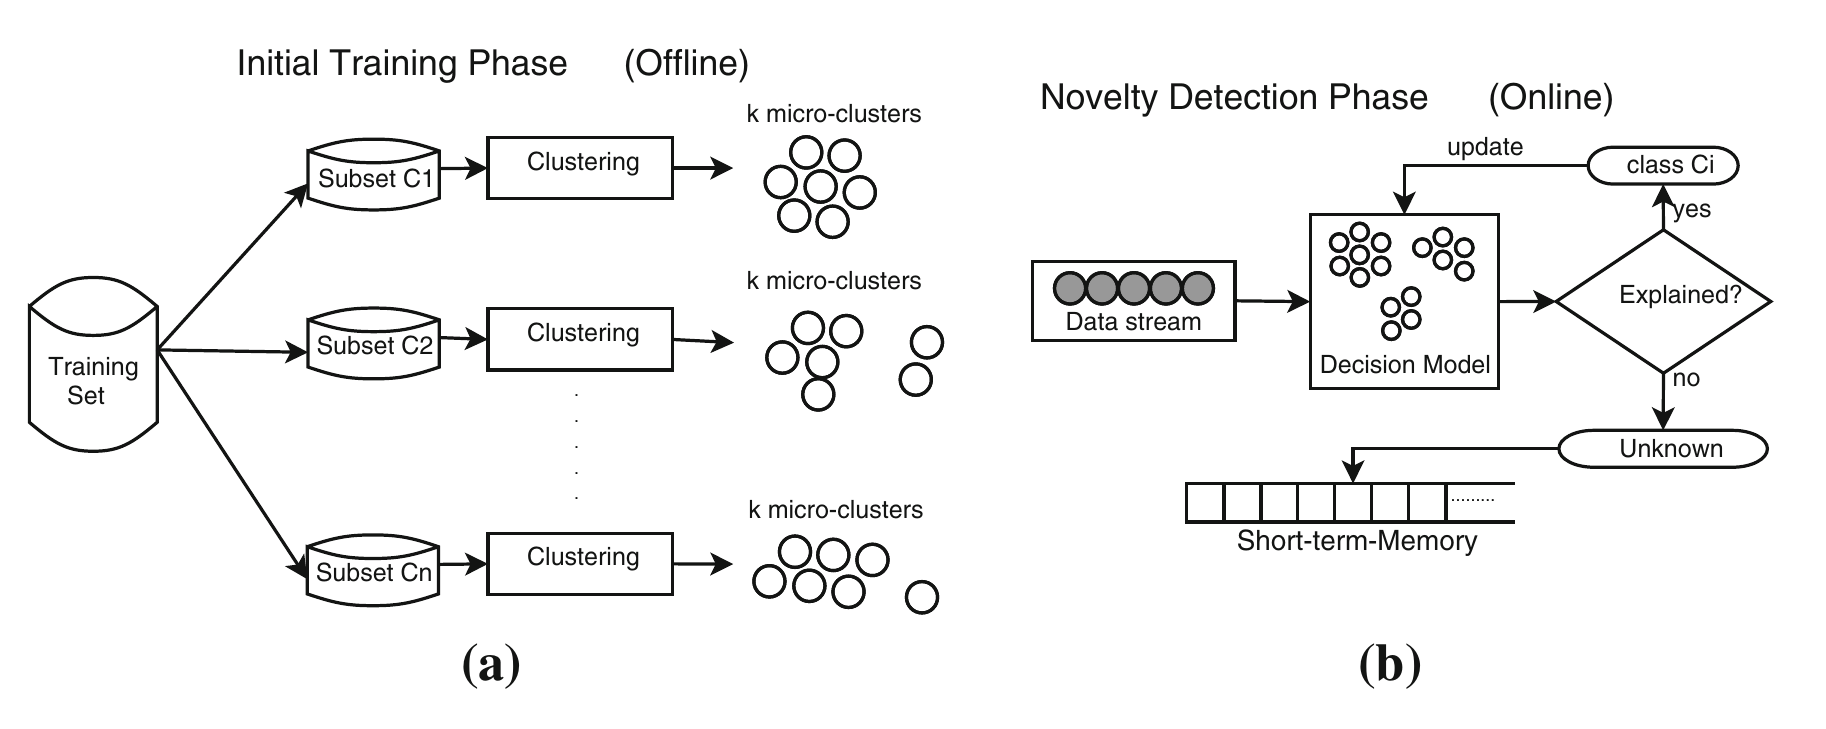
\includegraphics[width=1\textwidth]{figuras/FariaMinas2015-fases.png}
\caption{Visão geral do algoritmo MINAS com fases \emph{Offline} (a) e 
\emph{Online} (b) \cite{Faria2016minas}}
\label{fig:minas}
\end{figure}

\newcommand{\mcluster}{\emph{micro-cluster}\xspace}
\newcommand{\mclusters}{\emph{micro-clusters}\xspace}

% \nota{talvez mencionar que o minas trabalha no dominio de Double[]}

O algoritmo MINAS em sua fase \emph{Offline} consome um conjunto treinamento
contendo exemplos etiquetados.
Esse conjunto de treinamento é dividido em grupos usando como chave a etiqueta,
e para cada grupo de exemplos o método de agrupamento (\emph{clustering}) é executado.
O método de agrupamento objetiva resumir um conjunto maior de exemplos em 
um conjunto menor de \mclusters que representem por meio de um sumário
contendo, entre outras estatísticas, o centro e raio.
A cada \mcluster é adicionada a etiqueta do grupo original e todos
os conjuntos são unidos formando o modelo de decisão.

Na fase \emph{Online}, listada no Algoritmo \ref{alg:MINAS}, o algoritmo MINAS
opera com dois métodos.
O primeiro método é o de classificação, onde exemplos do fluxo de dados
são consumidos e avaliados pelo modelo de decisão.
O modelo de decisão avalia cada exemplo calculando a distância euclideana
entre o exemplo e todos \mclusters do modelo, selecionando o
\mcluster de menor distância.
Se a distância entre o exemplo e o centro do \mcluster for menor que
o raio do \mcluster o exemplo é classificado com a etiqueta do \mcluster
e o sumário estatístico do \mcluster é atualizado.
Caso a distância seja maior o exemplo é marcado como desconhecido e armazenado
em conjunto próprio.

O segundo método da fase \emph{Online} é a detecção de padrões novidade
que é executada quando o tamanho do conjunto de desconhecidos é maior
que um parâmetro predefinido.
Esse método executa o agrupamento (\emph{clustering} descrito na fase
\emph{Offline}) e valida os \mclusters gerados verificando sua representatividade
e coesão.

\begin{algorithm}[ht]
  \caption{MINAS \cite{Faria2016minas,Cassales2019a}}
  \label{alg:MINAS}
  \renewcommand{\algorithmicrequire}{\textbf{Entrada:}}
  \begin{algorithmic}[1]
    %T = limiar de distância para pertencer ao grupo
    %P = tempo de "inatividade" para passar para memória sleep
    %ts = limiar para remoção de exemplos da memória temporária
    \REQUIRE $Modelo,FCD,T,NumMinExemplos,ts,P$
    \STATE $MemTmp \leftarrow \emptyset$
    \STATE $MemSleep \leftarrow \emptyset$
    \FORALL{$exemplo \in FCD$}
    \STATE $(Dist,micro) \leftarrow$ micro-mais-proximo($exemplo,Modelo$)
    \IF{$Dist < $ raio($micro$)}
    \STATE $exemplo.classe \leftarrow micro.rotulo$
    \STATE atualizar-micro($micro,exemplo$)
    \ELSE
    \STATE $exemplo.classe \leftarrow desconhecido$
    \STATE $MemTmp \leftarrow MemTmp \cup exemplo$
    \IF{$|MemTmp| \geq NumMinExemplos$}
    \STATE $Modelo \leftarrow $ deteccao-novidade($Modelo,MemTmp,T$)
    \ENDIF
    \ENDIF
    \STATE $TempoAtual \leftarrow exemplo.T$
    \IF{$TempoAtual$ mod $TamJanela == 0$}
    \STATE $Modelo \leftarrow$ mover-micro-grupos-mem-sleep($Modelo,MemSleep,P$)
    \STATE $MemTmp \leftarrow$ remover-exemplos-antigos($MemTmp,ts$)
    \ENDIF
    \ENDFOR
  \end{algorithmic}
\end{algorithm}

Para atribuição de etiquetas aos \mclusters gerados o algoritmo MINAS
encontra no modelo atual o \mcluster mais próximo pela distância
euclidiana e classifica em dois tipos de conceito.
Se a distância é menor que um parâmetro predefinido,
o novo \mcluster gerado recebe como etiqueta o valor de extensão
de conceito conhecido.
Caso contrário, se o novo \mcluster está mais distante,
um novo conceito foi encontrado e a etiqueta marca uma novidade.
Após a atribuição da etiqueta do novo \mcluster, ele é adicionado
ao modelo de decisão.

% Although efficient in detecting NP, MINAS is
% very sensitive to noisy data and data scale, what causes a
% decrease in its accuracy. \cite{DaSilva2018}

% ver paper da profa. Elaine

% % discussão de 2020-02-01
% Detecção de intrusão em redes
%     - riscos de segurança
%     % pontos de coleta de dados básicos para a maioria das estruturas de IoT sao Wireless Sensor Networks (WSN) e WSN baseadas em IP,
%     % as quais s˜ao vulneráveis e geram uma ameac¸a de seguranc¸a de alto n´ıvel (ADAT; GUPTA, 2018) Adat2018
%     % (KASINATHAN et al., 2013), a detecc¸ ˜ao de assinaturas
%     % (RAZA; WALLGREN; VOIGT, 2013; SHEIKHAN; BOSTANI, 2016) s˜ao propostos IDSs h´ıbridos com foco 
%                 % espec´ıfico em ataques de roteamento como sink-hole e redireciona- mento seletivo
%     - técnicas de intrusão e tipos de ataques
%     - mecanismo de detecção (análise de fluxo de rede -> detecção de anomalia)
%     % Guilherme: A tarefa de detecção de intrusão consiste em descobrir, 
%     %           determinar e identificar a utilização, duplicação, alteração ou destruição
%     %           não autorizada de sistemas de informação (MUKKAMALA; SUNG; ABRAHAM, 2005) Mukkamala2005
%     % deteccao por assinaturas (tambem chamada de misuse-detection), deteccao comportamental (tambem chamada de anomaly-detection)e deteccao hıbrida.(MODI et al., 2013).
%     % implementacao usualmente é feita por meio de técnicas de AM e MD (BUCZAK; GUVEN, 2016).
%     % existem poucos trabalhos [..] online e deteccao de novidade ao problema [..] observado nas surveys (BUCZAK; GUVEN, 2016; MITCHELL; CHEN, 2014; MODI et al., 2013).
%     % (FURQUIM et al., 2018), os autores implementam uma arquitetura de 3 camadas (WSN, Fog e Cloud)
%     % (MIDI et al., 2017), os autores propuseram um IDS h´ıbrido [...] ativa apenas os módulos [...] especializado em um ataque espec´ıfic
%     % (FAISAL et al., 2015)externo ou interno ao Smart Meter.dados do KDD99 [...] precis˜ao, Kappa, consumo de memória, tempo e FAR
%     % extensivamente em (Sommer; Paxson, 2010) e (MCHUGH, 2000), é dif´ıcil encontrar boas me- didas de avaliac¸ ˜ao para IDSs
%     % (GAMA, 2010) afirma que no contexto de processamento de fluxo, as medidas tradicionais s˜ao impreci- sas.
% Detecção de novidades
%     % (PERNER, 2007)(GAMA, 2010). A
%     - técnicas de Detecção de novidades
%     - MINAS (incluir métricas) 
%     % (FARIA et al., 2016)
%     % ECSMiner (MASUD et al., 2011)
%     % AnyNovel (ABDALLAH et al., 2016) s˜ao
%     % medidas de Qualidade da Deteccao utilizadas foram Fnew, Mnew, Erro e a quantidade de exemplos rotulados por especialistas que cada técnica requisitou (MASUD et al., 2011)
%     - BigFlow (incluir métricas)
% Processamento de Streams (big data)
%     - cloud?
%     % A arquitetura Lambda (MARZ; WARREN, 2015) de duas camadas de CPU (stream e batch) e camada de serviço
%     % Kappa (KREPS, 2014) possui apenas um módulo de processamento on-line (apenas as camadas de processamento e servic¸o)
%     - redes como stream
%     - Atraso
%     - Kafka/Spark/Flink
% Redes IoT
%     - Restrição hardware (Energia, CPU, Mem, Rede)
%     - Consideração FOG vs Cloud
% %/discussão

% \clearpage

\section{Detecção de Novidade}\label{sec:nd}

\newcommand{\novelty}{\emph{Novelty Detection}\xspace}
\newcommand{\drift}{\emph{Concept Drift}\xspace}
\newcommand{\evolution}{\emph{Concept Evolution}\xspace}

% \notafa{(senteça marcada) Alguns autores consideram novidade e anomalia como a
% mesma coisa. Outros não (eu sou um dos que não considera)}
No âmbito de classificação de dados, parte da área de aprendizado de máquina, os
métodos de detecção de novidade (\novelty, \nd) lidam com o reconhecimento e a 
classificação \hlke{de exemplos que diferem de
exemplos anteriores} \cite{PERNER2007,Gama2010}.
Esses métodos tratam da classificação em fluxos de dados que evoluem com o
tempo, levando em consideração as características desse tipo de fluxos.

% \nota{"As características desse tipo de fluxo de dados são?".. mas que tipo?}

Tratando-se de fluxos de dados contínuos, são características
\notahl{quais?}dos \hlhl{padrões observados}:
evolução de conceito (\evolution) em que novos padrões podem surgir;
desaparecimento ou recorrência de conceito, em que padrões podem desaparecer e
também podem reaparecer;
mudança de conceito (\drift, também nomeado deriva ou desvio) onde um padrão
gradualmente se transforma;
presença de ruído e \emph{outliers} \cite{Gama2010}.

% \nota{separar ai - ndpara\\
% padroes novidade? reconhecomemnto de padroes novidade?}

Os métodos de \nd são aplicados a diversos problemas como
detecção de intrusos \cite{Coull2003,Spinosa2008,Viegas2019,Cassales2019a},
detecção de falhas \cite{Zhang2006},
diagnósticos médicos \cite{Perner2009},
detecção de regiões de interesse em imagens \cite{singh2004approach},
detecção de fraudes \cite{wang2003mining,Abdallah201690}, 
filtros de spam \cite{Hayat2010dct} e
detecção de variações comportamentais em um jogador \cite{Vallim20136258}.

% breve descrição do que sao algoritmos para DN

\nota{TODO: terminar reescrita}
Alguns métodos de \nd utilizam 
\notafa{frase estranha}
tratam de novidades como uma classificação de uma
ou duas classes () onde um conceito representa a classe normal e
as 
\hlfa{anomalias são representadas}
\hlfa{pela falta de conceito no modelo} ou
como um segundo conceito no modelo.
Além da abordagem de classificação binária, 
% não é adequada para representar
% \notafa{alguns trabalhos fazem isso, mas nem todos. É importante destacar que
% isso é a visão de um grupo de autor.}
\hlfa{múltiplos conceitos}
em um mesmo conjunto de dados, para isso é necessário abordar
\nd como classificação multi-classe.
Alguns métodos que abordam \nd como classificação multi-classe não
atendem completamente características de conjuntos com 
\notafa{o que é evolução temporal?}
\hlfa{evolução temporal,}
como \evolution e \drift, deixando de detectar múltiplos padrões que surgem
simultaneamente num intervalo de avaliação \cite{Faria2016nd,Gama2010}.

% \notafa{um grupo de algoritmos fazem isso, mas nem todos}
A maioria dos métodos de \nd são construídos seguindo a abordagem de aprendizado
\emph{Offline-Online}. Essa abordagem estabelece que o método seja dividido em
duas fases:
a primeira fase (\emph{Offline}) usa um conjunto de exemplos rotulados para
deles extrair conceitos conhecidos e gerar um modelo;
a segunda fase (\emph{Online}) consome um conjunto ou fluxo de exemplos não
rotulados e detecta padrões-novidade.
Além de detectar padrões-novidade, alguns algoritmos classificam cada exemplo
em um dos conceitos do modelo, ou marca o exemplo como desconhecido.
Ainda na segunda fase, para atualizar o modelo, os exemplos marcados como
desconhecidos são utilizados para a extração de novos conceitos ou variações em
conceitos conhecidos \cite{Gama2010}.

Dentre os métodos de \nd que baseiam-se em aprendizado \emph{Offline-Online},
muitos são baseados em algoritmos de agrupamento não supervisionados, tanto
para construção do modelo inicial como na extração de novos conceitos dos
exemplos não explicados pelo modelo marcados como desconhecidos
\cite{Spinosa2009ollinda,Masud2010ECSMiner,Faria2013}.

% Essa abordagem se deve as características 

% \cite{Gama2007,Gama2010,Masud2010ECSMiner,Faria2013,Lavin2015,Abdallah2016anynovel}.

% \cite{Costa2019thesis}

%     - técnicas de Detecção de novidades
% ver se tem algum survey e citar
% (PERNER, 2007)(GAMA, 2010)
% ECSMiner (MASUD et al., 2011)

\subsection{O algoritmo MINAS}\label{sec:minas-og}

Um algoritmo de \nd que tem recebido atenção nos últimos anos é o algoritmo
MINAS, originalmente proposto por \citeonline{Faria2013}, refinado por
\citeonline{Faria2015minas} e recentemente aprimorado por
\citeonline{DaSilva2018thesis}, com o uso de conceitos \emph{Fuzzy}, e expandido por
\citeonline{Costa2019thesis}, para tratar problemas multi-rótulo além dos problemas
multi-classe já tratados na versão original.
Esse algoritmo segue a abordagem de duas fases no modelo \emph{Offline-Online} e
usa por base algoritmos de agrupamento não supervisionados como \emph{K-means} e
\emph{CluStream}.
% As duas fases, com exceção do método de detecção de padrões novidade da fase
% \emph{Online}, são ilustradas na \reffig{minas}.

% \begin{figure}[ht]
% \centering
% 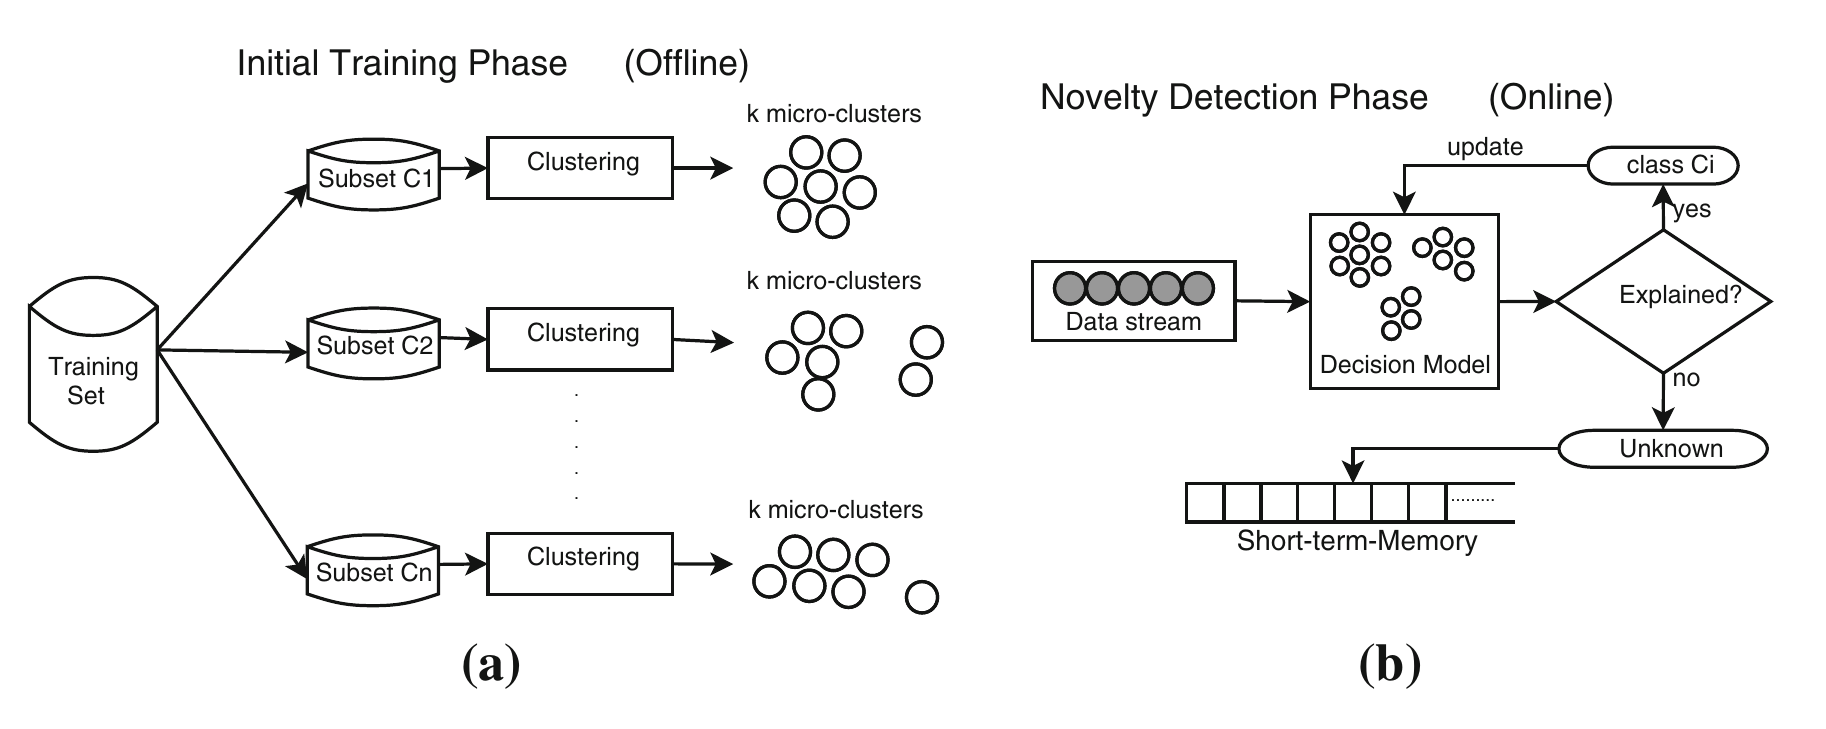
\includegraphics[width=1\textwidth]{figuras/FariaMinas2015-fases.png}
% \caption{Visão geral do algoritmo MINAS com fases \emph{Offline} (a) e 
% \emph{Online} (b) \cite{Faria2015minas}}
% \label{fig:minas}
% \end{figure}

\newcommand{\mcluster}{\emph{micro-cluster}\xspace}
\newcommand{\mclusters}{\emph{micro-clusters}\xspace}

% \nota{talvez mencionar que o minas trabalha no dominio de Double[]}

O algoritmo MINAS em sua fase \emph{Offline} consome um conjunto de treinamento
contendo exemplos etiquetados.
Esse conjunto de treinamento é dividido em grupos usando como chave a etiqueta,
e para cada grupo de exemplos o método de agrupamento (\emph{clustering}) é executado.
O método de agrupamento objetiva resumir um conjunto maior de exemplos em
um conjunto menor de \mclusters.

% \notafa{essas estatisitcas podem ser deduzidas pelos sumario, mas nao sao o sumario}
Um \mcluster é uma tupla de quatro components $(N, \mathbf{LS}, \mathbf{SS}, T)$
derivados dos exemplos representados por este \mcluster, onde:
$N$ número de exemplos,
$\mathbf{LS}$ soma linear dos exemplos,
$\mathbf{SS}$ soma quadrada dos exemplos,
$T$ instante de chegada do último exemplo adicionado ao \mcluster.
Deste sumário extrai-se, entre outras estatísticas, o centro e raio que são
utilizados na operação de classificação da fase \emph{Online}.
A cada \mcluster é adicionada a etiqueta do grupo original e todos \mclusters
são arranjados em um único conjunto formando o modelo de decisão.

Na fase \emph{Online}, listada no Algoritmo \ref{alg:MINAS}, o algoritmo MINAS
opera com três operações: classificação de novos exemplos, detecção de 
padrões-novidade e atualização do modelo de decisão \cite{Faria2015minas}.
O primeiro método é o de classificação, onde exemplos do fluxo de dados
são consumidos e avaliados pelo modelo de decisão.
O modelo de decisão avalia cada exemplo calculando a distância euclidiana
entre o exemplo e todos \mclusters do modelo, selecionando o
\mcluster de menor distância.
Se a distância entre o exemplo e o centro do \mcluster for menor que
o raio do \mcluster, o exemplo é classificado com a etiqueta do \mcluster
e o sumário estatístico do \mcluster é atualizado.
Caso a distância (mínima no modelo) seja maior que o raio,
o exemplo é marcado como desconhecido e armazenado
em conjunto próprio \cite{Faria2015minas}.

O segundo método da fase \emph{Online} é a detecção de padrões novidade,
que é executada quando o tamanho do conjunto de desconhecidos é maior
que um parâmetro predefinido.
Esse método executa o agrupamento (\emph{clustering} descrito na fase
\emph{Offline}) e valida os \mclusters gerados verificando sua representatividade
e coesão.

\subsection{MINAS}
\label{sec:minas}

\minas \cite{Faria2013Minas,Faria2015minas} is an offline-online \nd algorithm,
meaning it has two distinct phases. The first phase (offline) creates an initial
model set with several clusters based on a clustering algorithm with a training
set.
Each cluster can be associated with only one class of the problem, but each
class can have many clusters.

During its online phase, which is the main focus of our work, \minas performs
three tasks in (near) real-time,
in summary,
classification, novelty detection, and model update tasks
in a potentially infinite data stream, as shown in Algorithm \ref{alg:minas-main}.

\minas attempts to classify each incoming unlabeled instance according to the
current decision model. Instances not explained by the current model
receive an \textit{unknown} label and are stored in an unknowns-buffer.
When the unknowns-buffer reaches a preset threshold, \minas executes the
Novelty Detection function.
After a set interval, samples in the unknowns-buffer are considered to be
noise or outliers and removed.
The algorithm also has a mechanism to forget clusters that became obsolete and
unrepresentative of the current data stream distribution, removing them from
the Model and storing in a Sleep Model for possible recurring pattern
detection \cite{Faria2015minas}.

\begin{algorithm}[ht]
  \caption{MINAS \cite{Faria2016minas,Cassales2019a}}
  \label{alg:MINAS}
  \renewcommand{\algorithmicrequire}{\textbf{Entrada:}}
  \begin{algorithmic}[1]
    %T = limiar de distância para pertencer ao grupo
    %P = tempo de "inatividade" para passar para memória sleep
    %ts = limiar para remoção de exemplos da memória temporária
    \REQUIRE $Modelo,FCD,T,NumMinExemplos,ts,P$
    \STATE $MemTmp \leftarrow \emptyset$
    \STATE $MemSleep \leftarrow \emptyset$
    \FORALL{$exemplo \in FCD$}
    \STATE $(Dist,micro) \leftarrow$ micro-mais-proximo($exemplo,Modelo$)
    \IF{$Dist < $ raio($micro$)}
    \STATE $exemplo.classe \leftarrow micro.rotulo$
    \STATE atualizar-micro($micro,exemplo$)
    \ELSE
    \STATE $exemplo.classe \leftarrow desconhecido$
    \STATE $MemTmp \leftarrow MemTmp \cup exemplo$
    \IF{$|MemTmp| \geq NumMinExemplos$}
    \STATE $Modelo \leftarrow $ deteccao-novidade($Modelo,MemTmp,T$)
    \ENDIF
    \ENDIF
    \STATE $TempoAtual \leftarrow exemplo.T$
    \IF{$TempoAtual$ mod $TamJanela == 0$}
    \STATE $Modelo \leftarrow$ mover-micro-grupos-mem-sleep($Modelo,MemSleep,P$)
    \STATE $MemTmp \leftarrow$ remover-exemplos-antigos($MemTmp,ts$)
    \ENDIF
    \ENDFOR
  \end{algorithmic}
\end{algorithm}


\begin{algorithm}[htb]
    % \DontPrintSemicolon
    \SetKwFunction{nearestCluster}{nearestCluster}
    \SetKwFunction{clustering}{clustering}
    \SetKwFunction{NoveltyDetection}{NoveltyDetection}
    \SetKwFunction{handleModelSleep}{moveToSleep}
    \SetKwFunction{removeOldSamples}{removeOldSamples}
    % 
    \SetKwProg{Function}{Function}{:}{}
    \SetKwFor{With}{with}{}{}
    \SetKw{continue}{continue}
    % 
    \KwIn{ModelSet, inputStream}
    \KwOut{outputStream}
    % 
    \SetKwData{cleaningWindow}{cleaningWindow}
    \SetKwData{noveltyDetectionTrigger}{noveltyDetectionTrigger}
    \SetKwInOut{KwParams}{Parameters}
    \KwParams{\cleaningWindow, \noveltyDetectionTrigger}
    % \KwSty{Parameters}: \cleaningWindow, \noveltyDetectionTrigger\\
    % 
    \SetKwFunction{MinasOnline}{MinasOnline}
    \Function{\MinasOnline{ModelSet, inputStream}}{
        UnkownSet $\leftarrow$ $\emptyset$, ModelSleepSet $\leftarrow$ $\emptyset$ \;
        lastCleanup $\leftarrow 0$ , noveltyIndex $\leftarrow 0$\;
        % sampleIn $\leftarrow 0$\;
        \ForEach{ {$sample_{i}$} $\in$ inputStream }{
            % sample.label $\leftarrow$ unknown\;
            % (distance, cluster) $\leftarrow$ \nearestCluster(sample, ModelSet)\;
            nearest $\leftarrow$ \nearestCluster(sample, ModelSet)\;
            \eIf{nearest.distance $<$ nearest.cluster.radius}{
                sample.label $\leftarrow$ nearest.cluster.label\;
                nearest.cluster.lastUsed $ \leftarrow i $ \;
            }
            {
                sample.label $\leftarrow$ unknown\;
                UnkownSet $\leftarrow$ UnkownSet $\cup$ sample\;
                \If{$|\;UnkownSet\;| \geq$ \noveltyDetectionTrigger}{
                    % \tcc{Novelty Detection}
                    novelties $\leftarrow$ \NoveltyDetection(ModelSet $\cup$ ModelSleepSet, *UnkownSet)\;
                    ModelSet $\leftarrow$ ModelSet $\cup$ novelties\;
                }
                \If{ $ i > $ ( lastCleanup $ + $ \cleaningWindow )}{
                    ModelSet $\leftarrow$ \handleModelSleep(ModelSet, *ModelSleepSet, lastCleanup)\;
                    UnkownSet $\leftarrow$ \removeOldSamples(UnkownSet, lastCleanup)\;
                    lastCleanup $ \leftarrow i $\;
                }
            }
            outputStream.append(sample)\;
        }
    }
\caption{Our interpretation of \minas baseado em \cite{Faria2015minas}}
\label{alg:minas-main}
\end{algorithm}

The Novelty Detection function, illustrated in Algorithm \ref{alg:MINAS-nd},
groups the instances to form new clusters, and each new cluster is validated to
discard the non-cohesive or unrepresentative ones.
Valid clusters are analyzed to decide if they represent an extension of a
known pattern or a completely new pattern. In both cases, the model absorbs the
valid clusters and starts using them to classify new instances.

\begin{algorithm}[htb]
    \SetKwProg{Function}{Function}{:}{}
    \SetKwData{minExamplesPerCluster}{minExamplesPerCluster}
    \SetKwData{noveltyFactor}{noveltyFactor}
    \SetKwInOut{KwParams}{Parameters}
    \KwParams{\minExamplesPerCluster, \noveltyFactor}
    % 
    \SetKwFunction{nearestCluster}{nearestCluster}
    \SetKwFunction{clustering}{clustering}
    \SetKwFunction{NoveltyDetection}{NoveltyDetection}
    \SetKwFunction{handleModelSleep}{moveToSleep}
    \SetKwFunction{removeOldSamples}{removeOldSamples}
    % 
    \Function{\NoveltyDetection{Model, Unknowns}}{
        newModelSet $\leftarrow$ $\emptyset$\;
        \ForEach{cl in \clustering(Unknowns)}{
            \If{$|\;cl.sampleSet\;| \geq$ \minExamplesPerCluster}{
                (distance, near) $\leftarrow$ \nearestCluster(cl, Model)\;
                \eIf{distance $<$ near.radius $\times$ \noveltyFactor}{
                    cl.label $\leftarrow$ near.label\;
                    cl.type $\leftarrow$ extension\;
                }{
                    cl.label $\leftarrow$ noveltyIndex\;
                    noveltyIndex $\leftarrow$ noveltyIndex $+ 1$\;
                    cl.type $\leftarrow$ novelty\;
                }
                Unknowns $\leftarrow$ Unknowns $-$ cl.sampleSet\;
                \label{alg:MINAS-nd:reclassify}
                newModelSet $\leftarrow$ newModelSet $\cup$ cl\;
            }
        }
        \Return{newModelSet}\;
    }
    \caption{\minas \cite{Faria2015minas} Novelty Detection task.}
    \label{alg:MINAS-nd}
\end{algorithm}

Para atribuição de etiquetas aos \mclusters gerados, o algoritmo MINAS
encontra no modelo atual o \mcluster mais próximo pela distância
euclidiana e classifica em dois tipos de conceito.
Se a distância é menor que um parâmetro predefinido,
o novo \mcluster gerado recebe como etiqueta o valor de extensão
de conceito conhecido.
Caso contrário, se o novo \mcluster está mais distante,
um novo conceito foi encontrado e a etiqueta marca um padrão novidade.
Após a atribuição da etiqueta do novo \mcluster, ele é adicionado
ao modelo de decisão.

% Although efficient in detecting NP, MINAS is
% very sensitive to noisy data and data scale, what causes a
% decrease in its accuracy. \cite{DaSilva2018}

% ver paper da profa. Elaine

% % discussão de 2020-02-01
% Detecção de intrusão em redes
%     - riscos de segurança
%     % pontos de coleta de dados básicos para a maioria das estruturas de IoT sao Wireless Sensor Networks (WSN) e WSN baseadas em IP,
%     % as quais s˜ao vulneráveis e geram uma ameac¸a de seguranc¸a de alto n´ıvel (ADAT; GUPTA, 2018) Adat2018
%     % (KASINATHAN et al., 2013), a detecc¸ ˜ao de assinaturas
%     % (RAZA; WALLGREN; VOIGT, 2013; SHEIKHAN; BOSTANI, 2016) s˜ao propostos IDSs h´ıbridos com foco 
%                 % espec´ıfico em ataques de roteamento como sink-hole e redireciona- mento seletivo
%     - técnicas de intrusão e tipos de ataques
%     - mecanismo de detecção (análise de fluxo de rede -> detecção de anomalia)
%     % Guilherme: A tarefa de detecção de intrusão consiste em descobrir, 
%     %           determinar e identificar a utilização, duplicação, alteração ou destruição
%     %           não autorizada de sistemas de informação (MUKKAMALA; SUNG; ABRAHAM, 2005) Mukkamala2005
%     % deteccao por assinaturas (tambem chamada de misuse-detection), deteccao comportamental (tambem chamada de anomaly-detection)e deteccao hıbrida.(MODI et al., 2013).
%     % implementacao usualmente é feita por meio de técnicas de AM e MD (BUCZAK; GUVEN, 2016).
%     % existem poucos trabalhos [..] online e deteccao de novidade ao problema [..] observado nas surveys (BUCZAK; GUVEN, 2016; MITCHELL; CHEN, 2014; MODI et al., 2013).
%     % (FURQUIM et al., 2018), os autores implementam uma arquitetura de 3 camadas (WSN, Fog e Cloud)
%     % (MIDI et al., 2017), os autores propuseram um IDS h´ıbrido [...] ativa apenas os módulos [...] especializado em um ataque espec´ıfic
%     % (FAISAL et al., 2015)externo ou interno ao Smart Meter.dados do KDD99 [...] precis˜ao, Kappa, consumo de memória, tempo e FAR
%     % extensivamente em (Sommer; Paxson, 2010) e (MCHUGH, 2000), é dif´ıcil encontrar boas me- didas de avaliac¸ ˜ao para IDSs
%     % (GAMA, 2010) afirma que no contexto de processamento de fluxo, as medidas tradicionais s˜ao impreci- sas.
% Detecção de novidades
%     % (PERNER, 2007)(GAMA, 2010). A
%     - técnicas de Detecção de novidades
%     - MINAS (incluir métricas) 
%     % (FARIA et al., 2016)
%     % ECSMiner (MASUD et al., 2011)
%     % AnyNovel (ABDALLAH et al., 2016) s˜ao
%     % medidas de Qualidade da Deteccao utilizadas foram Fnew, Mnew, Erro e a quantidade de exemplos rotulados por especialistas que cada técnica requisitou (MASUD et al., 2011)
%     - BigFlow (incluir métricas)
% Processamento de Streams (big data)
%     - cloud?
%     % A arquitetura Lambda (MARZ; WARREN, 2015) de duas camadas de CPU (stream e batch) e camada de serviço
%     % Kappa (KREPS, 2014) possui apenas um módulo de processamento on-line (apenas as camadas de processamento e servic¸o)
%     - redes como stream
%     - Atraso
%     - Kafka/Spark/Flink
% Redes IoT
%     - Restrição hardware (Energia, CPU, Mem, Rede)
%     - Consideração FOG vs Cloud
% %/discussão


% \subsection{Algoritmos de Detecção de Novidades}\label{sec:alg-nd}

\newcommand{\cluster}{\emph{cluster}\xspace}
\newcommand{\clusters}{\emph{clusters}\xspace}

\newcommand{\dataset}{\emph{data set}\xspace}
\newcommand{\datasets}{\emph{data sets}\xspace}
% \clusters é um conjunto de \cluster feito de um \dataset.

O algoritmo MINAS, como já foi discutido na Seção \ref{sec:minas-og}, classifica
exemplos e detecta
novidades em DS e considera em sua composição \emph{concept drift} e
\emph{concept evolution}, sendo capaz de classificar como extensão de classe
conhecida e identificar padrões novidade sem intervenção de especialista
\cite{Faria2015minas}.
Neste trabalho, consideram-se algoritmos derivados do algoritmo MINAS
aqueles apresentados em trabalhos publicados após 2016, que estendem a
implementação original seguindo sua estrutura básica.

\subsection{Algoritmo FuzzyND}

% FuzzyND
% $(n, \mathit{M}, \overline{CF1^x}, SSD^e, t, l)$
% $(n, LS, SS, t, l)$
% A nova estrutura contrapõem a estrutura original
% substituindo a soma linear dos elementos ($LS$) por  e $SS$ por $M$ e $$

O algoritmo FuzzyND, derivado do MINAS foi proposto por \citeonline{DaSilva2018}.
FuzzyND incrementa o algoritmo original, aplicando a ele teorias de
conjuntos \emph{fuzzy} pela modificação da representação dos \clusters.
A modificação afeta o método de construção de \clusters, método de classificação
de exemplos e método de detecção de novidades de acordo com a nova representação.

\acronym{F1M}{\emph{Macro F-Score}, acurácia }

A avaliação do algoritmo FuzzyND foi feita por meio de experimentos usando 3 
\datasets sintéticos (\emph{MOA3}, \emph{RBF}, \emph{SynEDC})
e por comparação com o MINAS.
O método de avaliação utilizado baseia-se na matriz de confusão incremental
descrita por \citeonline{Faria2016nd}, extraindo dessa matriz duas métricas:
acurácia (\emph{Macro F-Score}) \cite{Sokolova2009} e
taxa de desconhecidos (\emph{UnkR}) \cite{Faria2015minas}.
Em geral, o algoritmo FuzzyND detecta melhor novidades e, consequentemente,
é mais robusto a valores atípicos (\emph{outlier}), porém perde a capacidade
de reconhecer padrões recorrentes.


% Experiments were evaluated using the incremental confusion-matrix proposed by [27],
% recently been proposed [5]–[9]
% [5] T. Al-Khateeb, M. M. Masud, L. Khan, C. Aggarwal, J. Han, and B.
% Thuraisingham, “Stream classification with recurring and novel class detection
% using class-based ensemble,” in Data Mining (ICDM), 2012 IEEE 12th International
% Conference on. IEEE, 2012, pp. 31–40.
% [6] E. R. de Faria, A. C. P. de Leon Ferreira, J. Gama et al., “Minas:
% multiclass learning algorithm for novelty detection in data streams,” Data
% Mining and Knowledge Discovery, vol. 30, no. 3, pp. 640–680, 2016.
% [7] M. Masud, J. Gao, L. Khan, J. Han, and B. M. Thuraisingham, “Classification
% and novel class detection in concept-drifting data streams under time
% constraints,” IEEE Transactions on Knowledge and Data Engineering, vol. 23, no.
% 6, pp. 859–874, 2011.
% [8] M. M. Masud, Q. Chen, L. Khan, C. Aggarwal, J. Gao, J. Han, and B.
% Thuraisingham, “Addressing concept-evolution in concept-drifting data streams,”
% in Data Mining (ICDM), 2010 IEEE 10th International Conference on. IEEE, 2010,
% pp. 929–934.
% [9] Z. S. Abdallah, M. M. Gaber, B. Srinivasan, and S. Krishnaswamy, “Anynovel:
% detection of novel concepts in evolving data streams,” Evolving Systems, vol. 7,
% no. 2, pp. 73–93, 2016.
% [27] E. R. de Faria, I. R. Goncalves, J. Gama, A. C. P. de Leon Ferreira et al.,
% “Evaluation of multiclass novelty detection algorithms for data streams,” IEEE
% Transactions on Knowledge and Data Engineering, vol. 27, no. 11, pp. 2961–2973,
% 2015.
% [28] M. Sokolova and G. Lapalme, “A systematic analysis of performance measures
% for classification tasks,” Information Processing & Manage- ment, vol. 45, no.
% 4, pp. 427–437, 2009.

\subsection{Algoritmos MINAS-LC e MINAS-BR}\label{sub:minas-derivados}

O algoritmo MINAS-LC foi proposto por \citeonline{Costa2019thesis} e trata a classificação
multi-rótulo, porém não trata evoluções de conceito (\emph{Concept Evolution}).
As alterações fundamentais propostas são:
a representação de \cluster onde MINAS-LC troca a etiqueta, que era única, por uma multi-rótulo;
a transformação de problema aplicada ao conjunto de treinamento para transformá-lo de um
conjunto multi-rótulo para um conjunto multi-classe (simplificação)
em duas variações \emph{Label Powerset} e \emph{Pruned Sets} com
mineração de conjunto de itens frequentes.

% Este capítulo apresentou o método MultI-label learNing Algorithm for data
% Streams with Label Combination-based methods (MINAS-LC) e o MultI-label learNing
% Algorithm for data Streams with Binary Relevance transformation (MINAS-BR) para
% CMFCD com latência extrema de rótulos. O MINAS-LC lida com problemas apenas com
% mudanças de conceito. O seu modelo de decisão e composto por microgrupos
% multirrotulados sendo capaz de classificar exemplos em várias classes
% simultaneamente e evoluir ao longo do fluxo de dados. Foram propostas duas
% variações do método: utilizando o método de transformação de problema Label
% Powerset (LP) e, utilizando o método Pruned Sets (PS) com mineração de conjunto
% de itens frequentes. O MINAS-BR lida com problemas tanto com mudanças de
% conceito, como com evo- luções de conceito. Ele possui um conjunto de modelos de
% decisão, um para cada classe do problema. Esses modelos de decisão podem ser
% entendidos adaptando-se às mudanças de con- ceito, ou novos modelos de decisão
% podem ser criados, adaptando-se às evoluções de conceito. O próximo capítulo
% apresenta os experimentos realizados envolvendo os dois métodos propostos neste
% trabalho.

Já o trabalho de \citeonline{Costa2019}, estende o algoritmo original para que
classifique um exemplo com uma ou mais etiquetas usando a transformação
\emph{Binary Relevance}, o que deu origem ao algoritmo MINAS-BR.
O algoritmo modifica a representação do modelo, originalmente conjunto de \clusters, para
um grupo de \clusters por classe (etiqueta).
Também modifica o método de agrupamento, substituindo a inicialização do 
algoritmo \emph{K-means}, originalmente aleatória, pelo algoritmo 
\emph{Leader Incremental Clustering} \cite{Vijaya2004505}.

% as 4CRE-V13, 4CRE-V24 e 5CVT5 6 foram geradas originalmente em Souza et al. (2015b)
% SOUZA, V. M. A.; SILVA, D. F.; GAMA, J.; BATISTA, G. E. A. P. A. Data stream
% classification guided by clustering on nonstationary environments and extreme
% verification latency. In: Procee- dings ofSIAM International Conference on Data
% Mining (SDM). [S.l.: s.n.], 2015. p. 873–881. Citado 4 vezes nas páginas 17, 65,
% 87 e 89.

O algoritmo MINAS-BR também é experimentalmente avaliado com 4 \emph{data sets}
sintéticos: \emph{MOA-3C-5C-2D}, \emph{MOA-5C-7C-2D}, \emph{MOA-5C-7C-3} da
ferramenta MOA \cite{MOA} e \emph{4CRE-V2}
\footnote{
    A versão original do \dataset 4CRE-V2 está disponível em
    \url{https://sites.google.com/site/nonstationaryarchive/home}
}
gerados pelo método \emph{Radial Basis Function} \cite{souza2015,Costa2019}.
O algoritmo MINAS-BR foi comparado com 7 algoritmos da literatura também
disponíveis na ferramenta MOA \cite{MOA}, diferente da avaliação do FuzzyND que
compara diretamente com MINAS. Para análise, os 7 algoritmos foram divididos em
dois grupos \cite{Costa2019}.
O primeiro grupo de 3 algoritmos com acesso às etiquetas corretas para
atualização do modelo e com a técnica ADWIN (\emph{ADaptive WINdowing}) para detectar
mudanças de conceito (\emph{Concept Drift})
O segundo grupo com os 4 algoritmos sem acesso às etiquetas corretas,
ou seja, sem \emph{feedback} externo, mesma condição do MINAS-BR \cite{Costa2019}.

% Esse trecho parece mais fundamentação.

A avaliação elencada por \citeonline{Costa2019} leva em consideração que as classes
contidas no conjunto de testes podem não ter correlação direta com os padrões identificados
pelos algoritmos.
Para tratar a divergência, uma estratégia baseada em proposta anterior por
\citeonline{Faria2016nd} foi apresentada com alterações para exemplos multi-rótulo.
Após associação entre padrões de novidade e classes novidade foi possível calcular
métricas tradicionais.
A estratégia é executada na fase de classificação seguindo as regras:

\begin{enumerate}

    \item após o consumo do exemplo $X_n$;
    
    \item para todo padrão $P_i$ (etiqueta atribuída) identificado sem
    associação até o momento;
    
    \item com classes novidade $y_j$ (etiqueta real) presentes em exemplos antes
    $X_n$;
    
    \item preenche-se a tabela de contingência $\mathbf{T}_{(i,j)}$ relacionando
    padrão $P_i$ e classe $y_j$;
    
    \item calcula-se o grau de dependência $\mathit{F1}$ derivado da tabela de
    contingência $\mathit{F1}_{(i,j)} = f(\mathbf{T}_{(i,j)})$;
    
    \item valores $\mathit{F1}_{(i,j)} = 0$ são descartados;
    
    \item dentre os valores restantes: o padrão $P_i$ é associado à classe $y_j$
    se $\mathit{F1}_{(i,j)}$ é máximo.

\end{enumerate}

As métricas utilizadas por \citeonline{Costa2019} após a associação de classes e
padrões são as tradicionais taxa de desconhecidos (\emph{UnkRM}) e \emph{F1M}.
Os resultados apresentados indicam que MINAS-BR capturou todas as novidades dos
\datasets sintéticos de teste e mostrou, como esperado, melhores métricas que os
4 algoritmos equivalentes da literatura ficando abaixo dos 3 com \emph{feedback}
externo.

Os trabalhos abordados nessa \refsec{nd}, têm em
comum, além do algoritmo base, as métricas de avaliação acurácia (\emph{Macro F-Score} e \emph{Macro
F-Measure} F1M) e taxa de desconhecidos, aplicadas com devido tratamento.
Também é comum entre eles o uso de \datasets sintéticos.
Outro potencial não explorado do MINAS é em aplicações reais, ou seja,
consumindo além de \datasets reais, fluxos realistas em ambientes simulados ou
reais porém considerando uso de recursos computacionais.

Observando a arquitetura dos algoritmos abordados na \refsec{nd}, nota-se as semelhanças:
a fase offline centrada no processo de agrupamento e criação de modelo;
a fase online dividida em classificação (com atualização das estatísticas do modelo)
e detecção de padrões, onde novamente o processo de agrupamento é central.
Portanto, apesar de outros trabalhos expandirem o algoritmo com diferentes técnicas, seu
núcleo continua relevante\footnote{
Propostas de modificação do algoritmo MINAS estão longe de serem exauridas.
Não cabe ao presente trabalho expandir e validar conceitos de aprendizagem de máquina,
porém alguns exemplos mencionados ainda não abordados são:
\begin{enumerate*}[label={\alph*)}]
    
    \item diferentes métodos de cálculo de distância entre pontos além da
    distância euclidiana;
    
    \item a mudança de representação de \clusters, atualmente hiper-esferas
    \cite{Costa2019thesis}, para hiper-cubos tratando \datasets onde as
    características representadas pelas dimensões são completamente
    independentes;
    
    \item um modo interativo onde o \cluster é formado, mostrado ao especialista
    que o classifica como inválido (ruído ou não representativo) ou válido,
    podendo conter uma ou mais classes e, se contiver mais que uma classe corte em
    grupos menores até conter somente uma classe;
    
    \item ainda considerando interação com especialista, a possibilidade de
    injetar um exemplo não pertencente a uma classe, ou seja, marcar o exemplo
    como não pertencente a uma classe para mantê-lo na memória de
    desconhecidos e, eventualmente forçar criação de um \cluster que represente
    uma classe geometricamente próxima mas semanticamente distinta;
    
    \item na fase \emph{offline} a verificação de sobreposição de \clusters
    pertencentes a classes distintas e tratamento adequado.

\end{enumerate*}
} \cite{DaSilva2018,DaSilva2018thesis,Costa2019}.

% >>>>>>> master
% \citeonline{DaSilva2018}

% \citeonline{Costa2019} estende o algoritmo original na sua capacidade de
% classificar um exemplo com uma ou mais etiquetas usando a transformação
% \emph{Binary Relevance}. Essa versão modificada é testada e comparada com 7
% algoritmos por meio de experimentos com 4 \emph{data sets} sintéticos gerados
% pelo método \emph{Radial Basis Function}. Os 7 algoritmos e o método estão
% disponíveis na ferramenta MOA \cite{MOA}.
% w

% Apesar de outros trabalhos expandirem o algoritmo com diferentes técnicas, seu
% núcleo continua relevante \cite{DaSilva2018,DaSilva2018thesis,Costa2019}.
% <<<<<<

% \section{AnyNovel}
% \nota{Incompleto}

% \nota{também é da mesma classe do minas porém \citeonline{Cassales2019a} destaca um
% desempenho inferior para o \emph{data set} testado.}
%  a atividade de detecção de intrusão

% \citeonline{Abdallah2016anynovel}

% \nota{helio: Mining wireless networks}

% !TeX root = ./00.main.tex
\chapter{Trabalhos Relacionados}\label{cha:related}

% % discussão de 2020-02-01
% Aqueles que contenham:
%     - detecção de anomalia em streams
%     - detecção de intrusão em rede com processamento de streams
%     - BigFlow
% %/discussão

% cap 3: Trabalhos relacionados
%     - Artigos sobre o Minas
%     - outros que paralelizaram algoritmos de mineração de 
%        dados/streams alguns online (5-10 refs)
%     - implementação paralelas/distribuídas em dispositivos pequenos
% % 

\begin{resumocap}

Este Capítulo trata dos trabalhos relacionados e apresenta aspectos do estado da arte
dos tópicos Detecção de Novidades em Fluxos de Dados, e
Processamento Distribuído de Fluxos de Dados.
\notake{inserir uma tabela sumarizada com a descrição dos autores.}

\end{resumocap}

Nesta Capítulo, abordam-se trabalhos que aplicam \hlhl{algoritmos de detecção de
novidades} em \hlhl{ambiente de processamento distribuído} de fluxo de dados em tempo
real.
Um sumário dos trabalhos abordados pode ser visto na Tabela \ref{tab:summary}.

\newcommand{\kafka}{\emph{Apache Kafka}\xspace}
\newcommand{\flink}{\emph{Apache Flink}\xspace}
\newcommand{\spark}{\emph{Apache Spark}\xspace}
\newcommand{\python}{\emph{Python}\xspace}

\begin{table}[ht]
  \caption{Sumário dos trabalhos relacionados}
  \centering
  \begin{scriptsize}
%  \begin{tabularx}{\textwidth}{ l m{2cm} | m{2cm} l m{2cm} | m{2cm} | m{2cm} | m{2cm} }
  \begin{tabularx}{\linewidth}{X|X|X|X|X}
%  \begin{tabularx}{\textwidth}{l|l|X|X|m{3.0cm}}
    Trabalho & Plataforma  & Técnica & Conjunto de dados & Métricas \\
    \hline
    \hline
    Ferramenta BigFlow \cite{Viegas2019} &
        \python, \emph{flowtbag}, \kafka e \flink &
        Hoeffding Tree, OzaBoosting, Leveraging Bag e combinação &
        MAWILab &
        Acurácia (geral e por classe), Taxa de bytes \\
    \hline
    Ferramenta CATRACA \cite{Lopez2018} &
        \emph{Virtual Network Function}, \kafka e \spark &
        PCA, SFS, e SVM-RFE &
        NSL-KDD, GTA/UFRJ e NetOp &
        Acurácia, precisão, sensibilidade e F1-score \\
    \hline
    Arquitetura \idsiot \cite{Cassales2019a} &
        Java, \kafka e \python &
        ECSMiner, AnyNovel e MINAS &
        \emph{Kyoto 2006+} &
        Fnew, Mnew e erro \\
    \hline
    % \cite{dos-6lowpan-iot} & 6LoWPAN & Suricata & Dados reais com metasploit & Acurácia, pacotes/segundo\\
    % \cite{Hybrid-ids-arch-iot} & 6LoWPAN & Hibrida - MR OPF & NSL-KDD e ataque simulados & FAR e revocação \\
    % \cite{SVELTE} & 6LoWPAN & Análise de DAG & Sem informações & revocação, consumo de energia e memória\\
    % \cite{Fault-tolerance-disaster} & WSN & MLP do Weka & Dados reais & MAE, RMSE, R², R, acurácia, revocação, precisão, especificidade \\
    % \cite{Kalis} & WSN & Módulos independentes, cada qual com uma técnica & Replay de \textit{traces} e injeção de ataques & revocação, acurácia, consumo de CPU e memória\\
    % \cite{IoT-arch-smartmeter} & \textit{Smart City} & Agrupamento, MLP e modelos estatísticos & Dados reais dos medidores & Consumo de energia elétrica e água\\
    % \cite{scalable-anomaly-detection-smart-city} & Smart City & LiSA, função de suavização & Dados reais & \textit{Outliers}, comparação entre simulação e dados coletados\\
    % \cite{DS-based-IDS-SmartGrid} & \textit{Smart Grid} & 7 classificadores do MOA & KDD99 & Acurácia, \textit{Kappa}, consumo de memória, tempo, FAR e FNR \\
    % \cite{GT-BIS} & Big Data & Random Forest & Logs de servidores Http e MySQL & Acurácia \\
    %\cite{anomalies-adaptive-detection} & Big Data & Agrupamento, Algoritmos Genéticos e redução de atributos & KDD99 & Tempo, FAR, revocação, acurácia e memória \\
  \end{tabularx}
  \label{tab:summary}
  \end{scriptsize}
\end{table}

\section{Ferramenta BigFlow}

Proposta por \citeonline{Viegas2019}, a ferramenta BigFlow é um sistema de
detecção de intrusão em rede (\emph{Network Intrusion Detection System}, NIDS)
baseado em detecção de anomalias.
Duas abordagens, detecção por assinatura e detecção por anomalia, 
\notahl{?}\hlhl{são de uso frequente,}
\hlhl{como o mecanismo}
\hlhl{de detecção de intrusão na construção de NIDS}.
Para a detecção de novos tipos de ataque (\emph{zero day}), a abordagem de
detecção por anomalia é vantajosa, em contraste com a abordagem de detecção por
assinatura, devido ao tempo de resposta (que envolve a identificação e criação de
uma assinatura), grande demais para prevenir esse tipo de intrusão.

A ferramenta BigFlow é composta pelos módulos de extração de atributos e de aprendizado confiável.
O módulo de extração de atributos
% , ilustrado na \reffig{bigflow-pcap},
é responsável por coletar \hlhl{pacotes} da rede monitorada,
\notahl{extrair as características dos desses pacotes... não "transformar pacotes"...}
\hlhl{transformar esses pacotes em fluxos}
com estatísticas de comunicação e enviar informações desses fluxos como
exemplos para o módulo de aprendizado confiável.
O módulo de aprendizado confiável,
%  ilustrado na \reffig{bigflow-ml},
é composto pelos submódulos:
submódulo classificador, responsável por classificar exemplos;
submódulo de verificação, responsável por verificar o resultado de classificação;
submódulo de exemplos rejeitados, responsável por requisitar a um especialista
etiquetas para exemplos rejeitados e;
submódulo de atualização incremental, que atualiza e distribui o modelo aos classificadores.

% \begin{figure}[!h]
% \centering
% 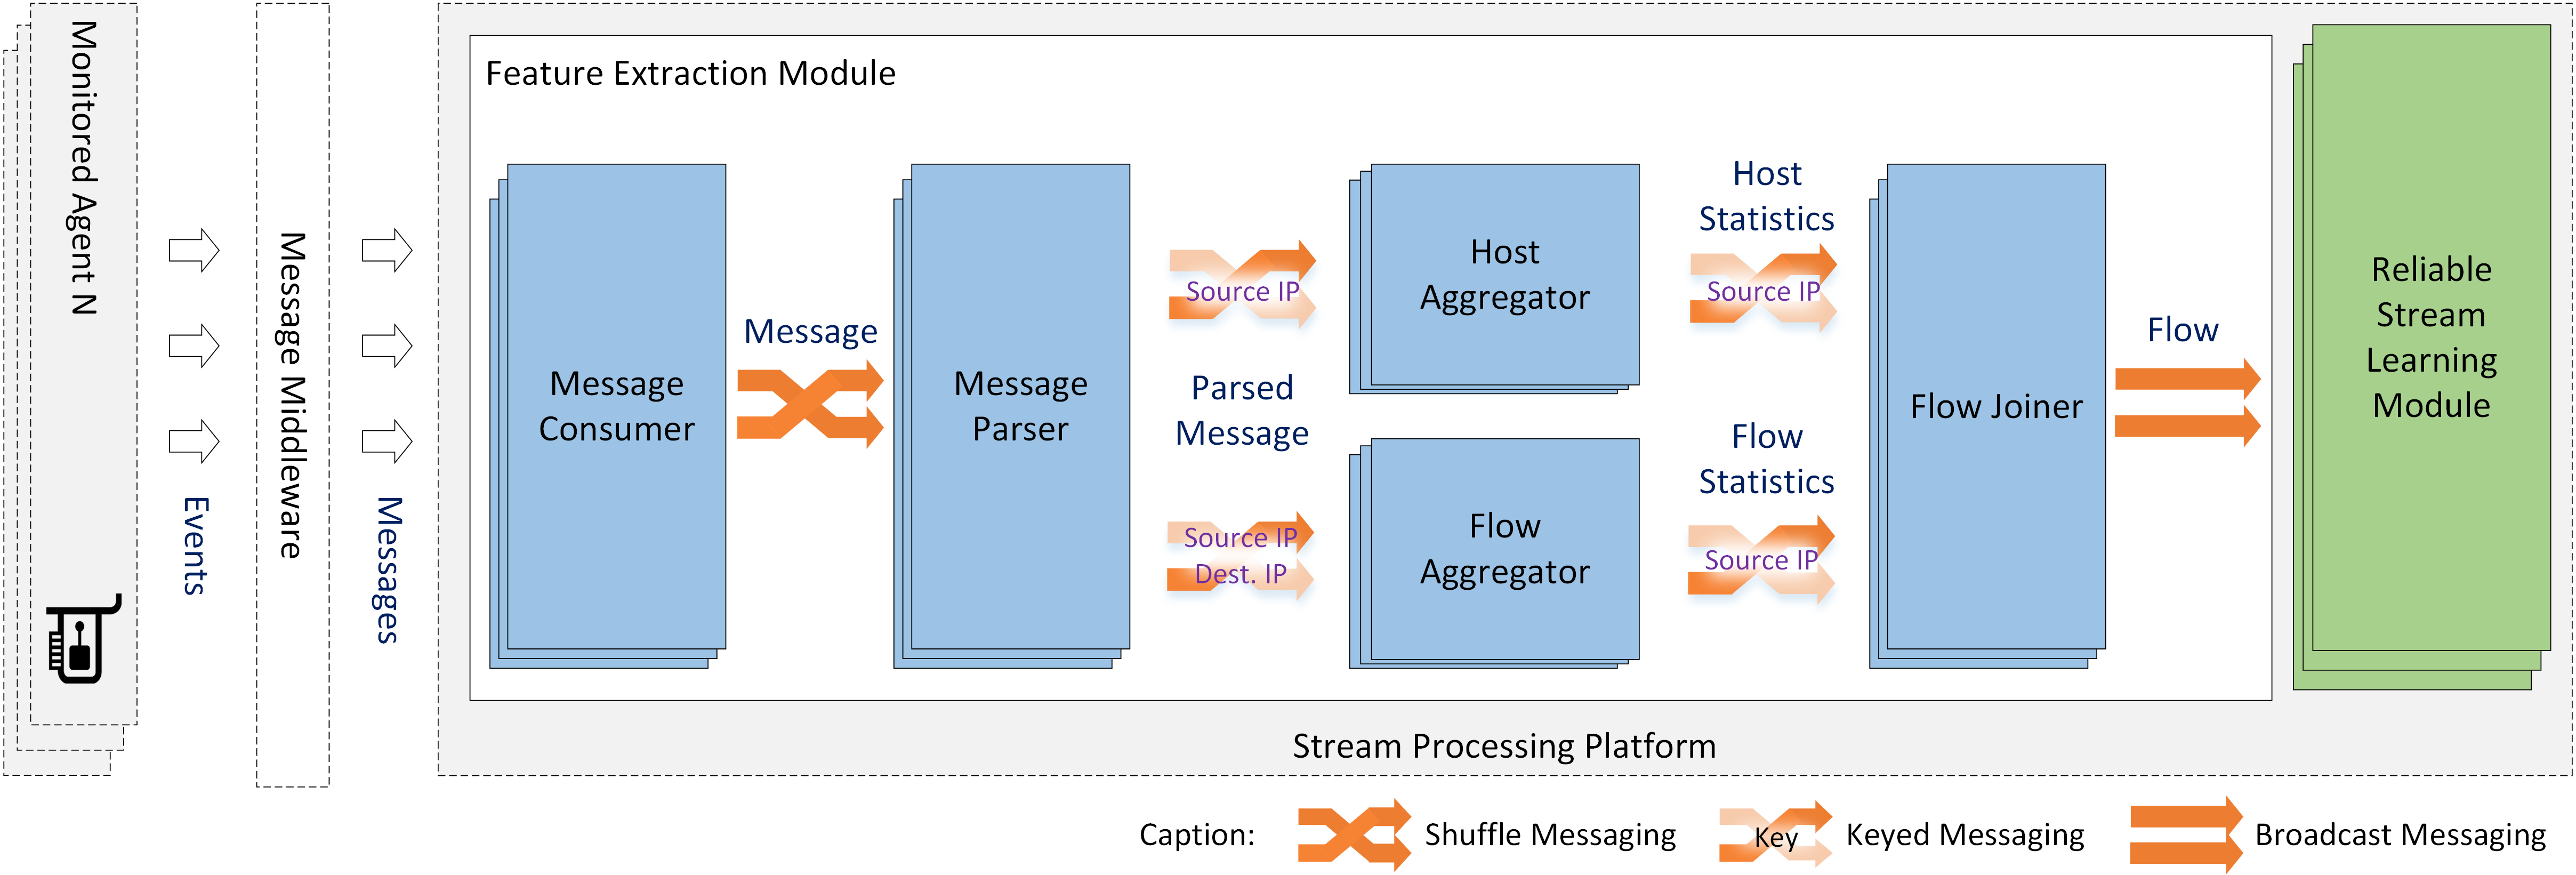
\includegraphics[width=\textwidth]{figuras/bigflow-fig2-feature_extraction_module.png}
% \caption{Módulo de extração de atributos da ferramenta BigFlow \cite{Viegas2019}.}
% \label{fig:bigflow-pcap}
% \end{figure}

% \begin{figure}[!ht]
% \centering
% 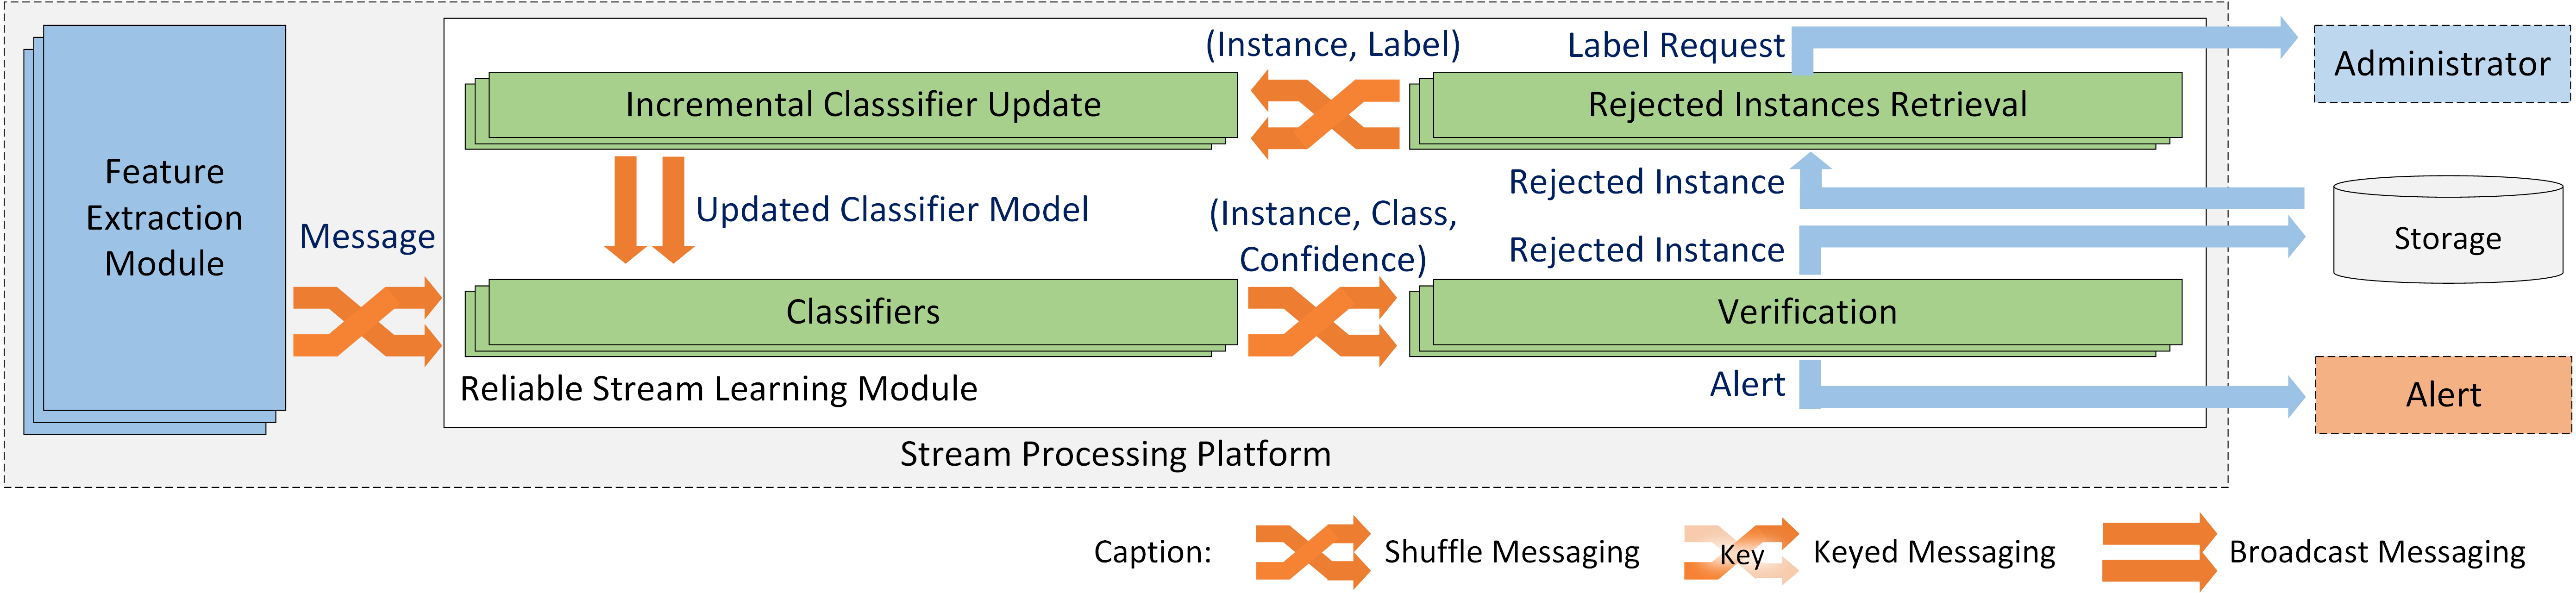
\includegraphics[width=\textwidth]{figuras/bigflow-fig4-reliable_learning_module.png}
% \caption{Módulo de aprendizado confiável da ferramenta BigFlow \cite{Viegas2019}.}
% \label{fig:bigflow-ml}
% \end{figure}

% BigFlow destaca em sua secção 2 (backgroud) o processamento de streams [18, 19],
% a preferencia de NIDS por anomalia em contraste aos NIDS por assinatura [30, 31, 32],
% a variabilidade e evolução dos padrões de tráfego em redes de propósito geral [9, 11, 20],
% a necessidade de atualização regular do modelo classificador [8, 9, 10, 20] e
% o tratamento de eventos onde a confiança resultante da classificação é baixa [9, 12, 13].

% [22] MAWI Working Group Traffic Archive, http://mawi.wide.ad.jp/mawi/samplepoint-F/.
% [24] H. He, E.A. Garcia, Learning from imbalanced data, IEEE Trans. Knowl. Data Eng.
% 21 (2009) 1263–1284. doi:10.1109/TKDE.2008.239.

\citeonline{Viegas2019} destaca que \datasets adequados para NIDS são
poucos, devido ao conjunto de qualidades que os mesmos devem atender, como
realismo, validade, etiquetamento, grande variabilidade e reprodutividade
(disponibilidade pública).

Para avaliar o desempenho de NIDS, o \dataset MAWIFlow é proposto por \citeonline{Viegas2019}.
Este \dataset é derivado do
\dataset \emph{Packet traces from WIDE backbone, samplepoint-F}, composto por
seções de captura de pacotes diárias de 15 minutos de um link de $1
\mathrm{Gbps}$ entre Japão e EUA, com início em 2006 continuamente até hoje,
anonimizados e etiquetados por MAWILab \cite{mawiSamplepointF,Fontugne2010}.
Desse \dataset original, o \dataset MAWIFlow utiliza apenas os eventos de 2016,
dos quais 158 atributos são extraídos resultando em 7.9 TB de captura de pacotes.
Além disso, os dados são estratificados para redução de seu tamanho a um
centésimo, \hlhl{mantendo} as proporções de etiquetas (Ataque e Normal), \hlhl{facilitando} o
compartilhamento e avaliação de NIDS, além de atender às qualidades anteriormente
mencionadas.

% classifiers that are usually employed for intrusion detection: decision tree
% (DT) [42], random forest (RF) [43], gradient boosting (GB) [44], and an ensemble
% [45] classifier composed from DT, RF, and GB that decides based on majority
% voting across each classifier’s decisions.

Com o \dataset MAWIFlow reduzido a 62 atributos, foram avaliados quatro
classificadores da literatura em dois modos de operação.
% quanto aoseus dados de treinamento (ambos contendo uma semana de captura).
O primeiro modo de operação usa somente a primeira semana do ano como conjunto
de treinamento e as demais como conjunto teste.
O segundo modo usa o conjunto da semana anterior como treinamento e o
conjunto da semana seguinte como teste.
Comparando os resultados entre os modos de operação, os autores demonstram que a qualidade da
classificação reduz-se com o tempo, quando não há atualização frequente do modelo
classificador.

Com base na avaliação dos classificadores da literatura, para a ferramenta
BigFlow é proposta a utilização de 4 algoritmos de classificação com capacidade
de atualização, sendo todos variações de árvore de decisão
\emph{Hoeffding} \cite{Viegas2019,Domingos2000}.
A avaliação da ferramenta foi executada de maneira semelhante à avaliação
dos algoritmos da literatura, onde o conjunto de dados da primeira semana foi
usado para treinamento e o conjunto de dados do restante do ano como conjunto
de teste.
Além do conjunto de treinamento, o modelo é atualizado semanalmente com base nas
instâncias rejeitadas pelo submódulo de verificação.
% , como ilustrado na \reffig{bigflow-ml}.

% four stream learning classifiers were evaluated:
% Hoeffding Tree [51], OzaBoosting [54], Leveraging Bag [55],
% and an Ensemble of the prior three classifiers that performs
% majority voting on the individual outcomes.

Quanto à distribuição do processamento,
%  ilustrada na \reffig{bigflow-arch},
a ferramenta BigFlow faz uso das plataformas \flink e \kafka.
Em especial, destaca-se o uso do serviço gerenciador de trabalhos (\emph{Job
Manager}) e as múltiplas instâncias do serviço gerenciador de tarefas
(\emph{Task Manager}).

% \begin{figure}[ht]
%   \centering
%   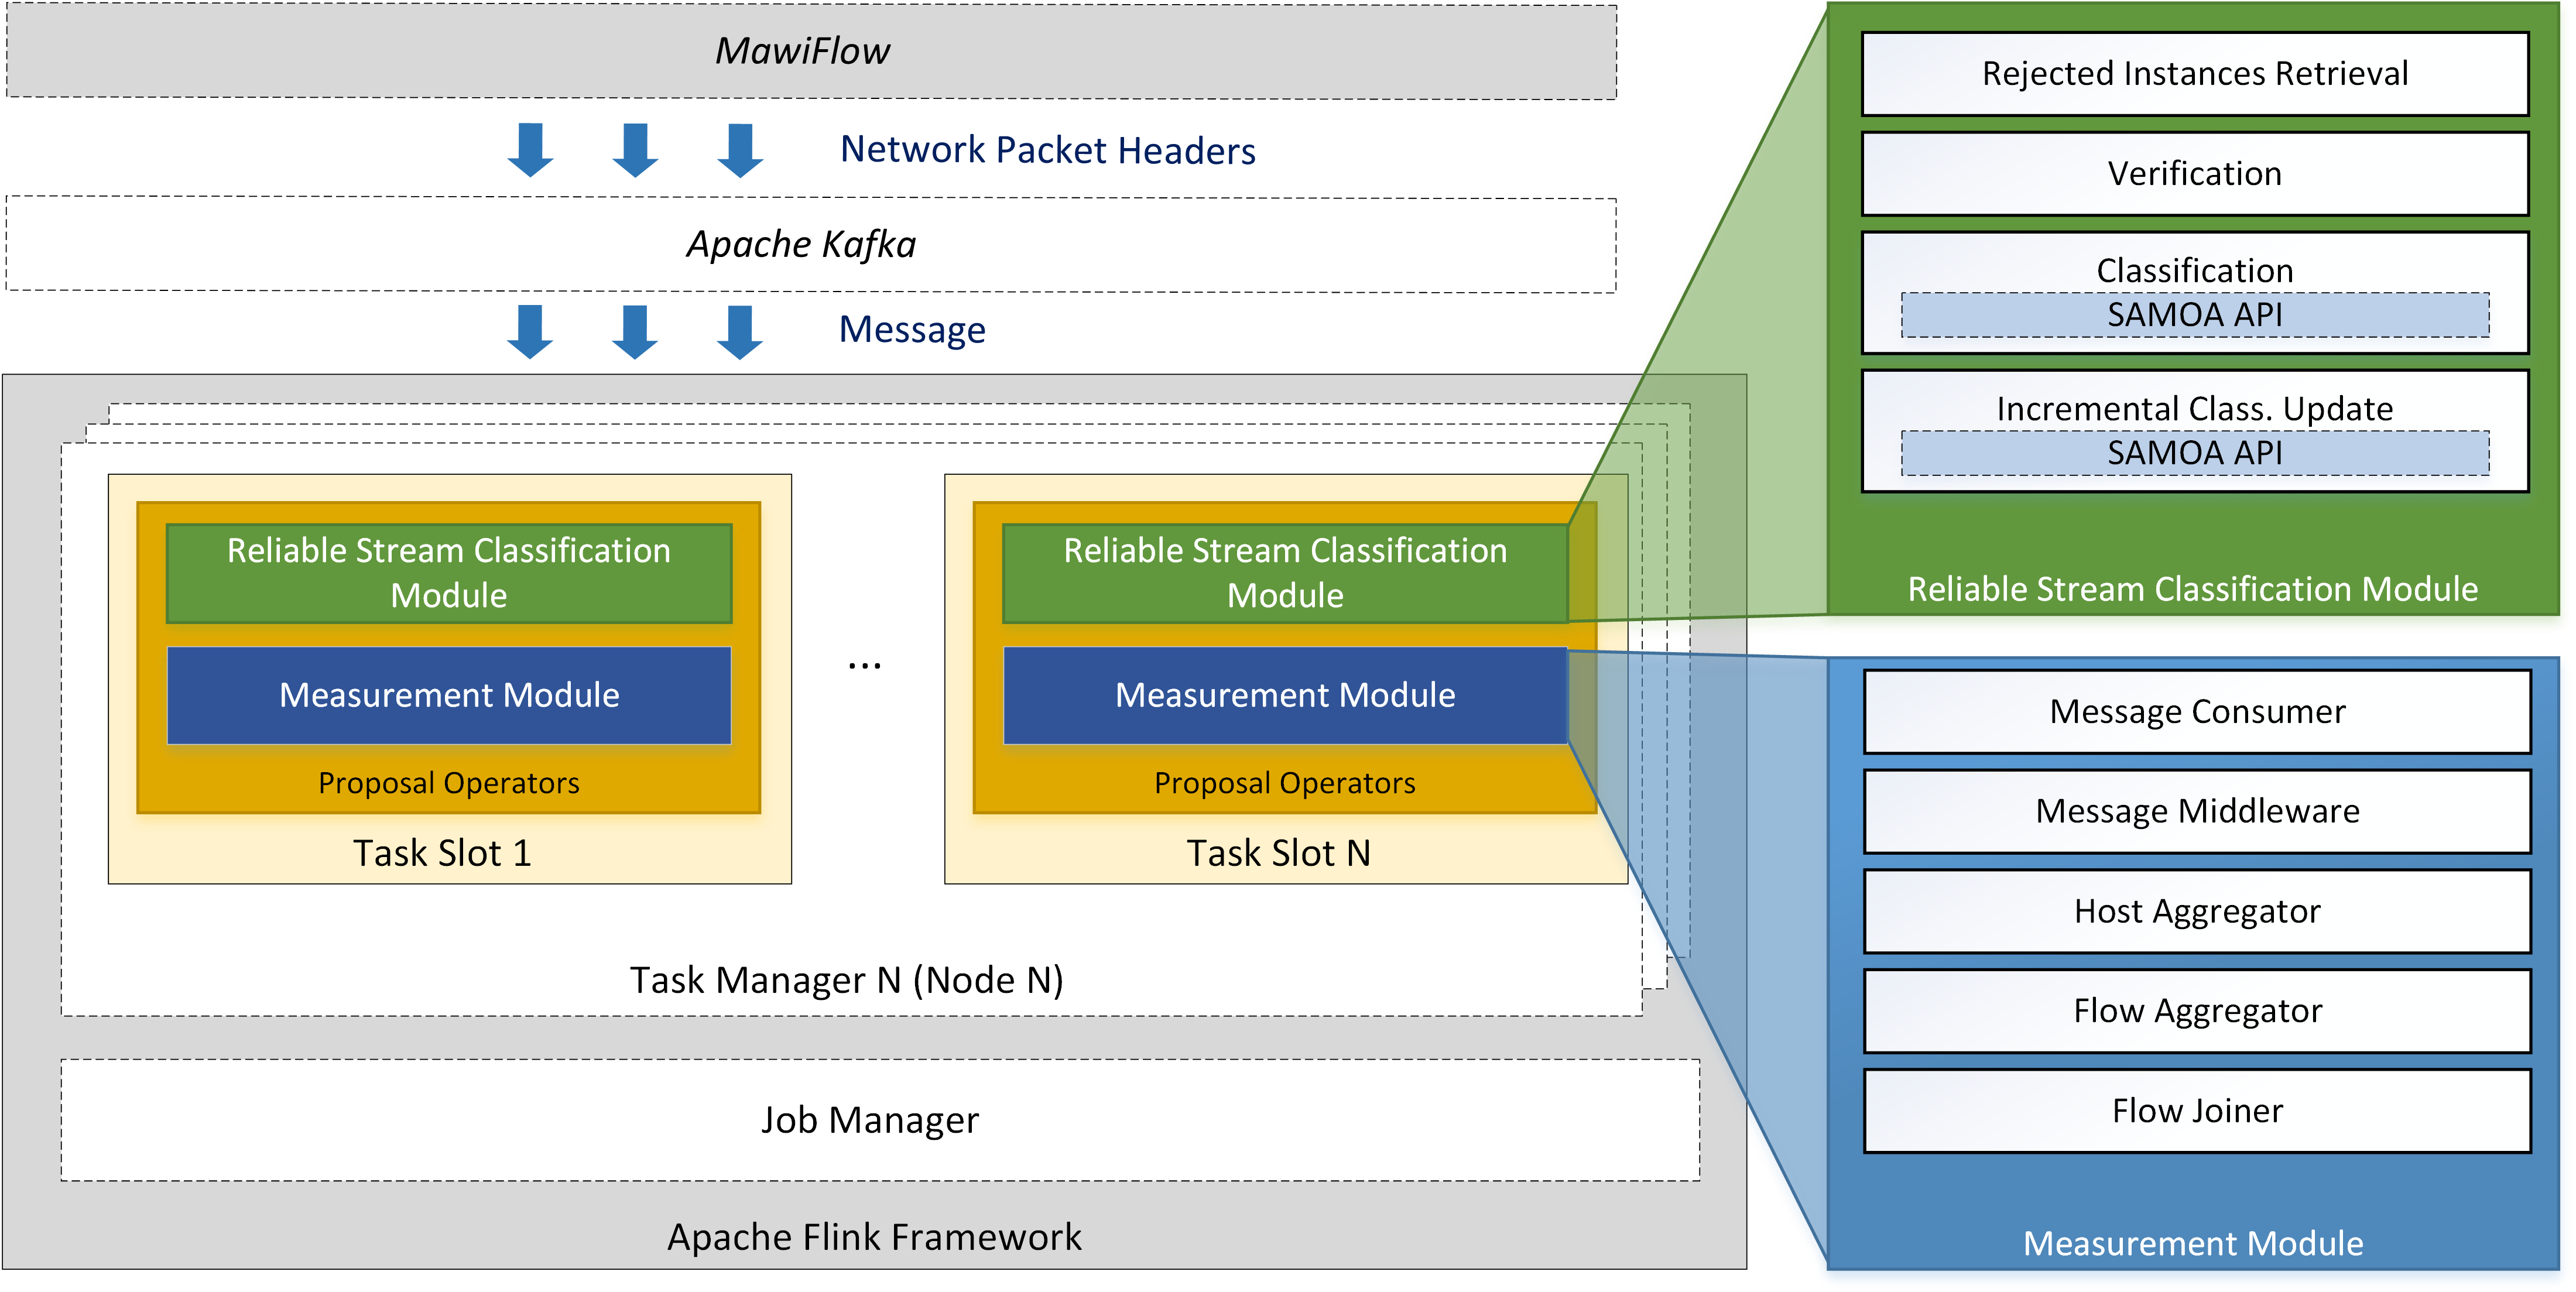
\includegraphics[width=\textwidth]{figuras/bigflow-fig5-bigflow_arch.png}
%   \caption{Visão geral da arquitetura e distribuição da ferramenta BigFlow \cite{Viegas2019}.}
%   \label{fig:bigflow-arch}
% \end{figure}

Em conclusão, a ferramenta BigFlow demonstra capacidade de classificação e
detecção de anomalias em fluxos de dados de alta velocidade no contexto de
detecção de intrusão.
\notahl{?}\hlhl{No entanto, a atualização semanal e, mais importante,}
\hlfa{dependendo de avaliação de}\\
\hlhl{um especialista não é ideal}
\hlhl{para detecção de novidades e}
\hlhl{respectiva ação sobre a descoberta}\\
\hlhl{de novos padrões.}

% Outras propostas tratam do caso de grandes volumes e velocidades, como ́e o caso
% de Viegas et al. (2019) que apresenta oBigFlow no intuito de detectar intrusão
% em redes10 GigabitEthernet, que ́e um volume considerável atualmente 
% impossível de ser processado em um ́único núcleo de processador (single-threaded).
% Essa implementação ́e feita sobre uma plataforma distribuída processadora
% de fluxos (Apache Flink) executada em um cluster com at ́e 10 n os de trabalho,
% cada um com 4 núcleos de processamento totalizando 40 núcleos para atingir
% taxas de até 10,72Gb ps.

\section{Ferramenta CATRACA}

O trabalho de \citeonline{Lopez2018} aborda a detecção de ameaças a redes de
computadores em tempo real e, para atingir esse objetivo, propôs a ferramenta
CATRACA\footnote{
    A ferramenta e sua documentação estão disponíveis em
    \url{http://gta.ufrj.br/catraca}
    e \url{https://github.com/tinchoa/catraca}.
}.
A ferramenta CATRACA é composta de três camadas: captura, processamento e
visualização.
%  ilustradas na Figura \ref{fig:catraca}.

% \begin{figure}[ht]
% \centering
% 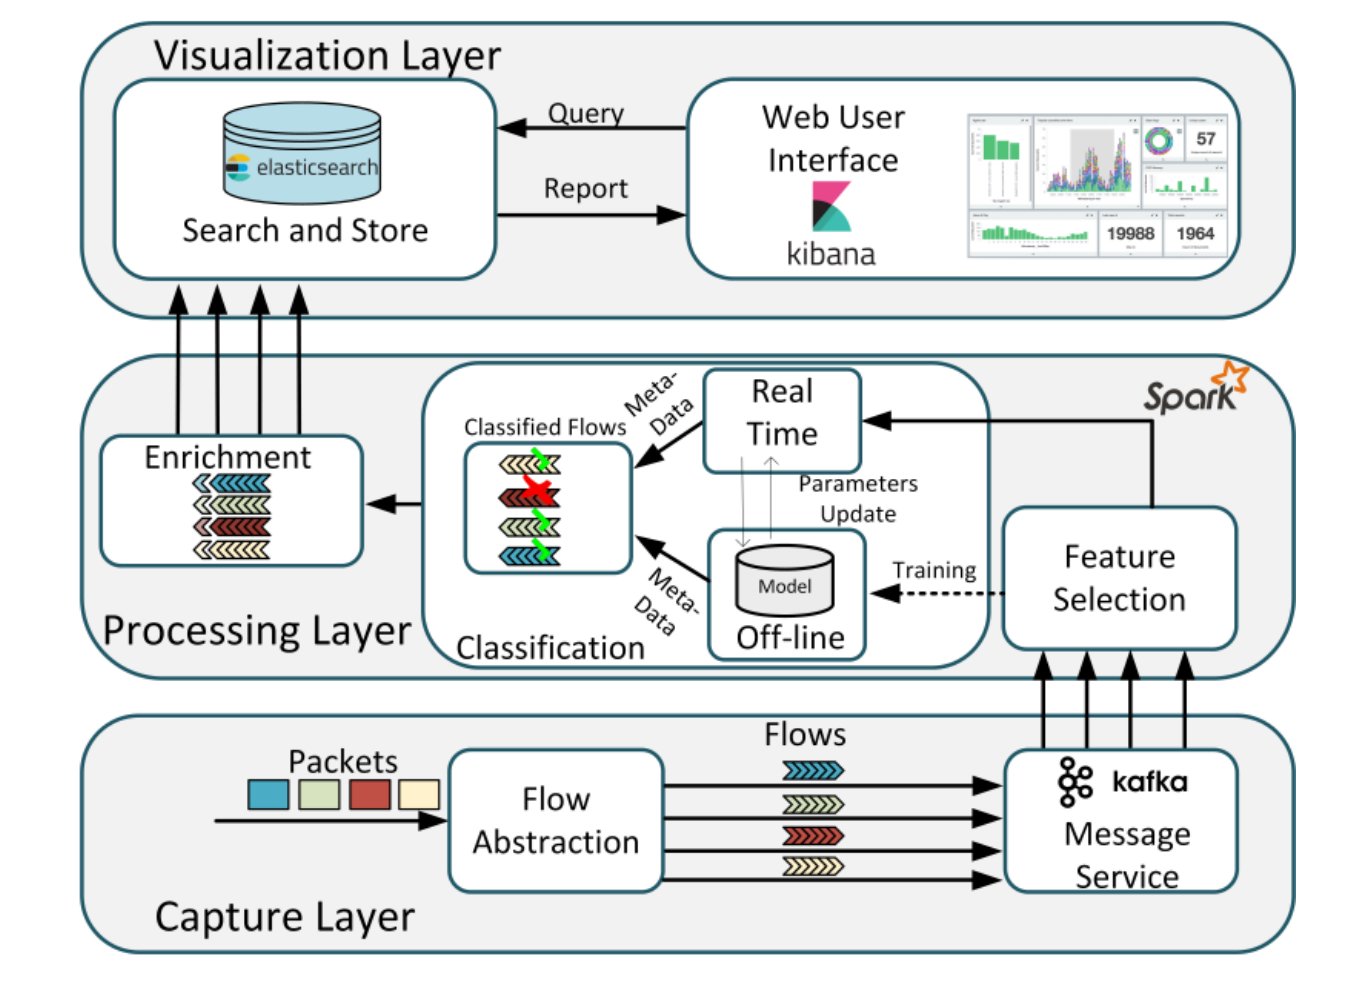
\includegraphics[width=0.8\textwidth]{figuras/catraca-arch.png}
% \caption{Arquitetura em camadas da ferramenta CATRACA \cite{Lopez2018}.}
% \label{fig:catraca}
% \end{figure}

% \nota{deu pra entender,mas coloca ou vírgula, ou divide as frases: baseada na
% biblioteca flowbag. Essa biblioteca é embalada ou a funcao em python esta
% embalada em um funcao virtual de rede?}

Na camada de captura, pacotes são capturados da rede e 
são geradas informações sumário de fluxos
por uma aplicação \emph{Python} utilizando a biblioteca \emph{flowtbag}\footnote{
    Disponível em \url{https://github.com/danielarndt/flowtbag} e
    \url{https://dan.arndt.ca/projects/netmate-flowcalc/}.
}.
Esses sumários são enviados para um tópico de um sistema de fila de mensagens
(\emph{Apache Kafka}) hospedado em nuvem.
Essa aplicação \emph{Python} é distribuída como uma função virtual de rede
(\emph{Network Function Virtualization}) executada em dispositivos de rede
virtuais.

% estabelecendo um ambiente de computação em névoa.
A camada de processamento consome o tópico de mensagens que contém os fluxos
da camada de captura e extrai características dos fluxos, detecta e classifica ameaças,
enriquece o resultado (com localização geográfica por exemplo) e envia para a
próxima camada na arquitetura por meio de um banco de dados (SGBD).
A última camada da ferramenta fornece uma interface gráfica que apresentada a
visualização dos fluxos processados bem como os conhecimentos extraídos e
armazenados no banco de dados (SGBD).
Ambas as camadas de processamento e visualização são executadas em ambiente de
computação em nuvem (\cloud).

Para o desenvolvimento da ferramenta CATRACA, \citeonline{Lopez2018} avaliou e
comparou as plataformas de processamento de fluxo de dados em tempo real
disponíveis (\emph{Apache Storm}, \emph{Apache Flink}, \emph{Apache Spark Streaming}).
A avaliação extraiu a velocidade máxima, em mensagens por minuto,
de cada plataforma, variando a configuração de paralelismo
em dois programas.
Ambos consumiam dados de um tópico de um sistema de fila
de mensagens (\emph{Apache Kafka}) e produziam para outro tópico.
O primeiro programa consiste de um detector de ameças composto por
uma rede neural classificadora escrito em \emph{Java}, que foi testado
com o conjunto de dados sintético UFRJ/GTA \cite{Lopez2018}.
O segundo programa conta quantas repetições de uma palavra existem em um
fluxo de dados, exemplo muito comum em tutoriais de plataformas desse gênero,
e é avaliado com um conjunto de \emph{Tweets}.

% Nesta avaliação, \emph{Apache Storm} foi capaz de processar até 15 milhões de
% mensagens por minuto
% 
% We described and compared the three-major open source distributed stream
% processing systems: Apache Storm, Apache Flink, and Apache Spark Streaming. We
% performed throughput analysis, allocating more processing cores to achieve
% higher processing rates, Apache Storm was able to process up to 15 million
% samples per minute. Moreover, we performed fault tolerance test to compare these
% three most popular open-source Distribute Stream Processors (DSP). In this case,
% we showed that Spark streaming, using micro-batch processing model, can recover
% the failure without losing any messages. Spark Streaming stores the full
% processing state of the micro-batches and distributes the interrupted processing
% homogeneously among other worker nodes.

% A comparação envolveu:
% \begin{enumerate}
%     \item Apache Storm versão 0.9.4 de 2015-03-18 (atualmente na versão 2.1.0,
%     publicada em 2019-10-25);
%     \item Apache Flink versão 0.10.2 de 2016-02-03 (atualmente na versão 1.10.0,
%     publicada em 2020-02-11);
%     \item Apache Spark Streams versão 1.6.1 de 2016-02-27 (atualmente na versão
%     2.4.5, publicada em 2020-02-02);
% \end{enumerate}
% Além das plataformas comparadas é importante mencionar a presença em todos os
% testes do Apache Kafka na versão 0.8.2.1 de 2015-02-26 (atualmente na versão
% 2.4.0 de 2019-12-13).
% A estratégia de avaliação continha um 
% Os resultados apresentados por essa avaliação mostraram que Apache Storm 

Para o modelo de classificação, a ferramenta CATRACA utiliza o método árvore de
decisão, escolhido pelo rápido treinamento e pela alta precisão e acurácia\footnote{
    A precisão e a acurácia do método árvore de decisão podem estar associadas
    à independência entre as características (\emph{features}) de cada exemplo,
    típico de conjuntos derivados de pacotes de rede.
}.
O modelo é criado na fase \emph{Offline} e utilizado na classificação binária
(normal e ameaça) da fase \emph{Online}, sendo recalculado quando uma ameaça
é encontrada.

% test\\
% $214200$\\
% $214\,200$\\
% $214\, 200$\\
% $214\;200$\\
% $214\; 200$\\
% $214200$\\

Pra avaliação da ferramenta CATRACA dois conjuntos de dados são utilizados.
O primeiro conjunto, UFRJ/GTA, é sintético e foi criado por uma simulação de
rede de computadores, contendo $214\;200$ fluxos de rede e totalizando $95
\mathrm{GB}$ de pacotes capturados, este \dataset
é composto de 24 atributos e 16 classes.
O outro conjunto, referido como NetOp, foi coletado de um operador de rede que
atendia 373 residências na cidade do Rio de Janeiro em 2017.
O conjunto NetOp é formado por 5 TB de pacotes capturados e etiquetados por um
detector de intrusão comercial.

Também para a avaliação da ferramenta CATRACA, foram utilizadas as métricas de qualidade
de classificação acurácia, precisão, sensibilidade e F1M, com intervalo de
confiança de 95\%.
As métricas de qualidade, dependendo do tamanho do conjunto, foram extraídas por
métodos de avaliação amplamente utilizados para avaliar modelos de aprendizado
de máquina (\emph{machine learning}) como validação cruzada com proporção
70\% do conjunto base para treinamento e 30\% para teste.
Para as métricas de escalabilidade foram utilizadas a latência e fator de aceleração
\emph{speedup factor} (latência observada com paralelismo 1 dividida pela
latência observada com paralelismo variável).

Em conclusão, a ferramenta CATRACA apresenta uma arquitetura dividida em camadas
alocadas em ambientes de névoa (\fog) e nuvem (\cloud).
Essa ferramenta foi avaliada com métricas de qualidade, métricas de
escalabilidade e dois conjuntos de dados relevantes.
No entanto, o algoritmo de detecção de anomalias desenvolvido para a ferramenta
consiste de um modelo de classificação pelo método árvore de decisão e
a atualização do modelo durante a fase \emph{Online} depende de todos os exemplos do
último intervalo de atualização.
Esse tipo de algoritmo de detecção de anomalias 
\notahl{por que não?}
\hlhl{não é capaz de lidar}
\hlhl{adequadamente com as características de fluxos contínuos} de dados, como os
descritos na \refsec{nd} (\drift, \evolution, limitado a ler o conjunto somente
uma vez), que são atendidos por algoritmos de detecção de novidade.

% A monitoring and threat detection system using stream processing as a virtual 
% function for Big Data

% A detecção tardia de ameaças de segurança causa um significante aumento no
% risco de danos irreparáveis, impossibilitando qualquer tentativa de defesa.
% Como consequência, a detecção rápida de ameaças em tempo real é essencial
% para a ad- ministração de segurança. Além disso, A tecnologia de
% virtualização de funções de rede (Network Function Virtualization - NFV)
% oferece novas oportunidades para soluções de segurança eficazes e de baixo
% custo. Propomos um sistema de detecção de ameaças rápido e eficiente,
% baseado em algoritmos de processamento de fluxo e de aprendizado de máquina. As
% principais contribuições deste trabalho são: 
% i) um novo sistema de monitoramento e detecção de ameaças baseado no processamento de fluxo; 
% ii) dois conjuntos de dados, o primeiro é um conjunto de dados sintético de
% segurança contendo tráfego suspeito e malicioso, e o segundo corresponde a uma
% semana de tráfego real de um operador de telecomunicações no Rio de Janeiro,
% Brasil; 
% iii) um algoritmo de pré-processamento de dados composto por um algoritmo
% de normalização e um algoritmo para seleção rápida de
% características com base na correlação entre variáveis;
% iv) uma função de
% rede virtualizada em uma plataforma de código aberto para fornecer um serviço
% de detecção de ameaças em tempo real;
% v) posicionamento quase perfeito de
% sensores através de uma heurística proposta para posicionamento estratégico
% de sensores na infraestrutura de rede, com um número mínimo de sensores; e,
% finalmente, 
% vi) um algoritmo guloso que aloca sob demanda uma sequência de 
% funções de rede virtual.

\section{Arquitetura \idsiot}\label{sec:cassales}

A arquitetura \idsiot, proposta por \citeonline{Cassales2019a}, tem por objetivo
monitorar uma rede local com dispositivos \iot e detectar tentativas de intrusão
e alguma subversão do comportamento das transmissões destes dispositivos.
O principal destaque da arquitetura é a distribuição de tarefas do sistema de
detecção de intrusão entre nós na \notahl{ou edge?}\hlhl{rede de borda (\fog)} e nós em nuvem pública
(\cloud).
O objetivo dessa distribuição é a redução de latência, que torna inviável a
hospedagem de um sistema detector de intrusão somente em ambiente \cloud, e
também possibilitar a análise de grandes volumes de dados por algoritmos de
maior complexidade, que são de custo computacional proibitivo para nós de borda.
A \reffig{ids-iot-phy} ilustra a estrutura física da arquitetura \idsiot,
destacando os dispositivos \iot, dispositivos de borda e nuvem pública.

\begin{figure}[ht]
\centering
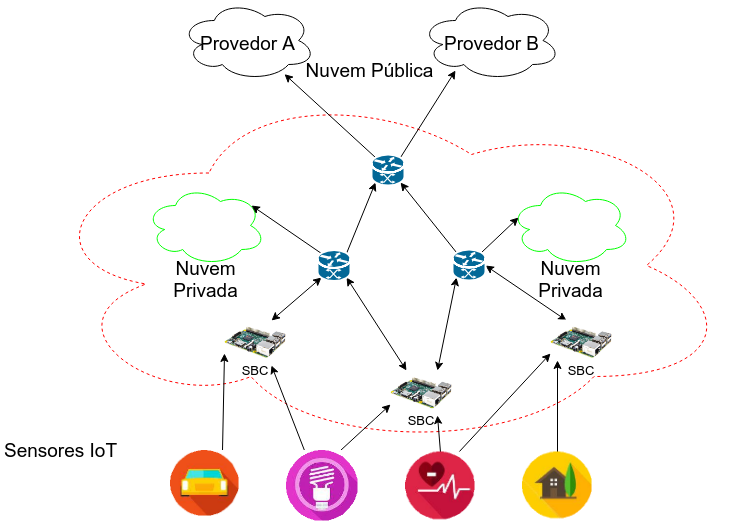
\includegraphics[width=0.8\textwidth]{figuras/idsa-iot-quali-000.png}
\caption{Estrutura Física da Arquitetura \idsiot.
Produzida e traduzida por \citeonline{Cassales2019a}.}
\label{fig:ids-iot-phy}
\end{figure}

A arquitetura proposta é avaliada com três algoritmos de detecção de novidade:
ECSMiner \cite{Masud2010ECSMiner}, AnyNovel \cite{Abdallah2016anynovel} e MINAS
\cite{Faria2016minas}.
A avaliação foi feita com o \dataset \emph{Kyoto 2006+}, composto de
dados coletados de 348 \emph{Honeypots} 
(máquinas isoladas, equipadas com diversos
softwares com vulnerabilidades conhecidas e expostas à Internet, com propósito de
atrair ataques) de 2006 até dezembro 2015.
Esse \dataset tem as características desejáveis de um conjunto para detectção de
novidades como: realismo, validade, etiquetas previamente definidas, alta
variabilidade, reprodutibilidade e disponibilidade pública.
O \dataset \emph{Kyoto 2006+} contém 24 atributos, 3 etiquetas atribuídas por
detectores de intrusão comerciais e uma etiqueta
distinguindo o tráfego entre normal, ataque conhecido e ataque desconhecido.

A avaliação da arquitetura foi realizada utilizando as métricas de qualidade
Fnew, Mnew e erro.
A métrica Fnew (ou Falso Positivo) é a fração dos exemplos de uma classe normal
classificados com etiqueta novidade ou etiqueta extensão.
A métrica Mnew (ou Falso Negativo) é a fração dos exemplos de uma classe novidade
classificados com etiqueta normal.
A métrica erro é a soma dos valores falso positivo e falso negativo dividida
pelo número de exemplos classificados.
Além das métricas de qualidade de classificação tradicionais, também foi medida
a quantidade de requisições de classificação por especialista.

Outra avaliação dos algoritmos foi a extração de métricas de uso de recursos
computacionais e tempo total de processamento em dispositivos limitados.
Essa avaliação envolveu dois computadores.
Para tanto, um computador pessoal com recursos
convencionais produzia exemplos e adicionava como mensagens em um tópico no
sistema de fila de mensagens \kafka; já o outro computador, com recursos
limitados, consumia as mensagens do tópico e classificava os exemplos.

Ambas as avaliações demonstraram o equilíbrio entre qualidade de classificação e
velocidade ou uso de recursos.
O algoritmo ECSMiner mostrou melhor qualidade de classificação, porém com
velocidade inferior e maior consumo de recursos comparado aos outros algoritmos.
Já o algoritmo MINAS, apesar de maiores valores na métrica erro, mostrou-se
adequado para dispositivos limitados com baixo consumo de recursos
computacionais e manteve a métrica Fnew constante e baixa.
O algoritmo AnyNovel não apresentou consistência nos resultados e o consumo
de recursos computacionais (memória) foi elevado.

% MINAS technique presented high error rates. However, the
% small and constant Fnew coupled with the smallest execution
% time and memory consumption, indicates MINAS is suitable
% for IoT scenarios.

Com as avaliações realizadas, a arquitetura \idsiot \hlhl{opta por distribuir} as
tarefas de mineração dos fluxos para detecção de intrusão em serviços e aloca os
serviços em diferentes camadas físicas, conforme ilustrado na \reffig{ids-iot}.

\begin{figure}[hbt]
\centering
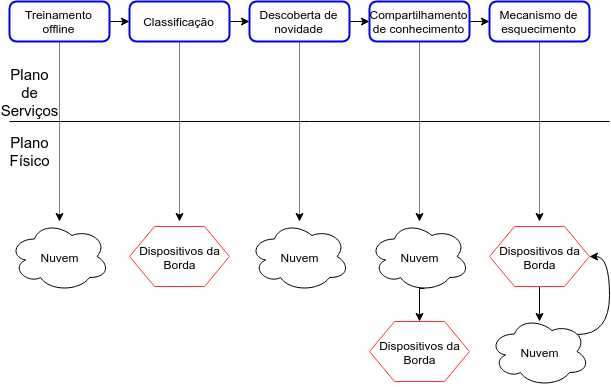
\includegraphics[width=0.8\textwidth]{figuras/idsa-iot-quali-004.png}
\caption{Distribuição de Serviços da Arquitetura \idsiot.
Produzida e traduzida por \citeonline{Cassales2019a}.}
\label{fig:ids-iot}
\end{figure}

A distribuição das tarefas em serviços proposta abre oportunidades para a
discussão de diferentes métodos de distribuição dessas tarefas em diferentes
ambientes computacionais.
Contudo, o algoritmo MINAS ainda não foi implementado e avaliado com
\hlhl{paralelismo, multi-processamento} ou \hlhl{distribuição computacional}, que são
necessários para tratar fluxos de dados com grandes volumes e velocidades.

% \nota{Também discutir a classificação dos fluxos por endpoint
% exarcerbando assim a distinção na fog com o efeito de particionamento dos dados.
% Ou seja, um nó só vê e classifica os próprios dados.}

% \section{Conjuntos de Dados e Referência de Desempenho para Detecção de Anomalia}

% The Numenta Anomaly Benchmark
% - Airline, approximately 116 million flight arrival and departure records
%   (cleaned and sorted) compiled by E. Ikonomovska. Reference: Data Expo 2009
%   Competition [1]. Access
% - Chess.com (online games) and Luxembourg (social survey) datasets compiled by
%   I. Zliobaite. Access
% - ECUE spam 2 datasets each consisting of more than 10,000 emails collected over
%   a period of approximately 2 years by an individual. Access from S.J.Delany
%   webpage
% - Elec2, electricity demand, 2 classes, 45,312 instances. Reference: M. Harries,
%   Splice-2 comparative evaluation: Electricity pricing, Technical report, The
%   University of South Wales, 1999. Access from J.Gama webpage. Comment on
%   applicability.
% - PAKDD'09 competition data represents the credit evaluation task. It is
%   collected over a five-year period. Unfortunately, the true labels are released
%   only for the first part of the data. Access
% - Sensor stream and Power supply stream datasets are available from X. Zhu's
%   Stream Data Mining Repository. Access
% - SMEAR is a benchmark data stream with a lot of missing values. Environment
%   observation data over 7 years. Predict cloudiness. Access
% - Text mining, a collection of text mining datasets with concept drift,
%   maintained by I. Katakis. Access
% - Gas Sensor Array Drift Dataset, a collection of 13,910 measurements from 16
%   chemical sensors utilized for drift compensation in a discrimination task of 6
%   gases at various levels of concentrations. Access

\newcommand{\stream}{\emph{data stream}\xspace}
\newcommand{\streams}{\emph{data streams}\xspace}
\newcommand{\streamMining}{\emph{data stream mining}\xspace}

\section{Conclusão}\label{sec:conclusao-relacionados}

% \nota{coloca uma secao de SINTESE dos trabalhos relacionados ou sintese do capitulo}

Em conclusão, os trabalhos discutidos nesse Capítulo têm temas complementares em
áreas distintas.
A área de aprendizado de máquina, com o tema detecção de novidades em fluxos de
dados, preocupa-se em fornecer melhores previsões através de algoritmos
classificadores que atendam as características de cada problema.
A área de computação distribuída aborda os temas de processamento distribuído
de fluxos contínuos em ambientes de computação em nuvem e em névoa, fornecendo
métodos para processar grandes volume de dados com mínima latência.

Apesar de já existirem propostas que estabelecem o estado da arte separadamente
em cada um dos temas, \hlhl{falta ainda uma abordagem que estabeleça uma união} entre o
estado da arte em \hlhl{algoritmos de detecção} de novidade e o estado da arte em
\hlhl{processamento distribuído} de fluxos de dados, em especial para \hlhl{o ambiente de
computação em névoa} focado em \hlhl{fluxos de dados} relacionados a \hlhl{dispositivos \iot.}

\notafa{
    você não discutiu sobre trabalhos anteriores que fizeram distribuição de
    algoritmos de fluxos de dados.... o que eles tem de bom e ruim (ex: trabalhos
    do Murilo Naldi da UFSCAR, trabalhos do Latifur, CLAM, trabalhos do Bifet e o
    framework baseado no MOA, mas distribuído)
}

% !TeX root = ./00.ppgcc-2020.tex

\chapter{Proposta e metodologia}\label{cha:proposta}

% \begin{resumocap}

  Este Capítulo apresenta a proposta deste trabalho e a metodologia elegida para
  atingir os objetivos.

% \end{resumocap}

In this work, we investigate an appropriate architecture for performing \nd at
the edge, as a means of allowing small IoT devices to filter and detect undesirable
network behavior.
Our approach is based on the \arch architecture \cite{Cassales2019a} and \nd
techniques provide by the \minas algorithm \cite{Faria2015minas}.
Named \mfog, our distributed algorithm explores load balancing to enable low
profile devices at the edge of the internet to also work on the classification
and detection of unwanted traffic.

In this work, we propose and assess \mfog, a distributed data stream
novelty detection system based on the algorithm \minas for securing \iot networks.
\mfog implements a distributed version of \minas according to the \arch
architecture proposed in a previous work \cite{Cassales2019a}, to execute in the
edge where small devices and constrained resources may be prevalent.

However, given the distributed nature and the typical use of small computing
devices in IoT scenarios, new challenges arise:

\begin{enumerate}[label=(\emph{\roman*})]
  \item the classification phase of the algorithm must occur in parallel at
  different nodes;
  \item the novelty detection phase, which provides the model evolution, must
  also be asynchronous;
  \item the algorithm complexity (time and space) must allow it to be processed
  by modest computing devices (i.e., small memory and low processor performance).
\end{enumerate}

\nids 
monitor network traffic, and analyze the characteristics of each flow 
to identify any intrusion or misbehavior.
However, this problem requires both fast and accurate response \cite{DaCosta2019a}:
fast response is needed to have a proper reaction before harm can be cast
to the network and to cope with the traffic without imposing loss or delay
in the \nids or observed network;
accurate response is required as not to misidentify,
especially the case of false positive that leads to false alarms.
To achieve those goals, we leverage fog computing.

In common \iot scenarios, data is captured by small devices and sent to the
cloud for any compute or storage tasks, but this is not feasible in a \nids
scenario.
Fog computing infrastructure aims to offload processing from the cloud
providers by placing edge devices closer to end-users and/or data sources.

In our proposal, fog and cloud computing resources are combined to minimize
the time elapsed between a flow descriptor ingestion and intrusion alarm,
performing the classification step of \minas running multiple
classifier instances.
After the initial classification, the resulting label can be used immediately,
but if the sample is labeled as \emph{unknown}, this sample must be stored and
the novelty detection step will be triggered.

% To have a better overview of our proposal and how it integrates with existing
% \iot environments, Figure \ref{fig:mfog-phy-arch-cloud} depicts such scenario
% showing from bottom to top:
% \iot devices directly connected to a (local) gateway network;
% this gateway network could be as simple as a single Internet router 
% or be more complex by connecting to private clouds or 
% containing more devices providing fog computing capabilities;
% lastly, available over the internet, the traditional public cloud provides
% inexpensive computing and storage on demand.
% In this scenario, the further apart resources are, the more network
% resources need to be employed, and, as with any networked system, the
% higher is the latency.

% \begin{figure}[hb]
%   \centering
%   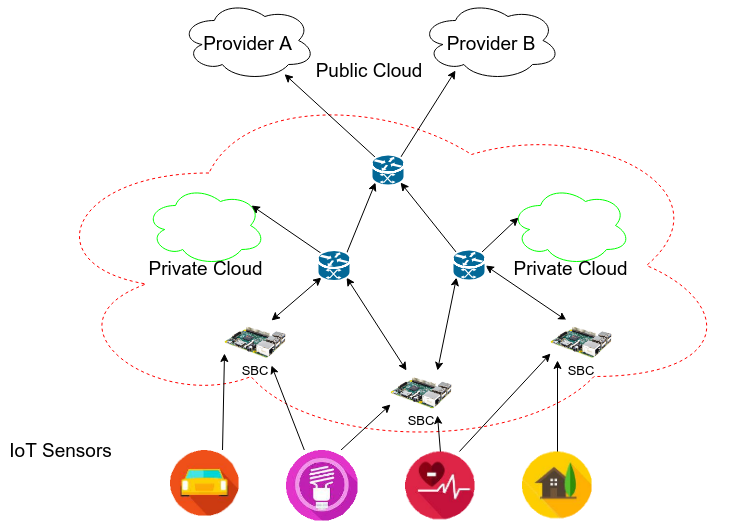
\includegraphics[width=0.5\linewidth]{figures/cassalesimgs-000.png}
%   \caption{\arch \cite{Cassales2019a} physical architecture and deployment scenario overview.}
%   \label{fig:mfog-phy-arch-cloud}
% \end{figure}

The overall \mfog architecture has two main modules, Classification and Novelty
Detection, which implement the \minas main tasks.
The Classification Module performs the same task of the \minas Online phase and
is the focal point for parallelism and distribution in our proposal.
It is replicated in the fog and runs on each cluster node, using a configurable
number of threads (limited to the node CPU core count).

The Novelty Detection Module can also be replicated,
the choice being one instance per local network, one global cloud instance,
or both.
This module also handles the homonymous task of \minas Online phase, receiving
all the samples labeled with \emph{unknown}, storing them in an internal
\emph{unknown-buffer}, and, when this buffer is full, performing the \minas
Novelty Detection task (clustering followed by validation).

\section{Polices}\label{sec:polices}

The design of our distributed \nd architecture includes partitioning the
functionalities of \minas and establishing the appropriate data flows
between different actors.
Changes to placement and behavior can have different impacts and should be
chosen with care.
The decisions following these discussions can be organized in several policies,
some of them were recurring during our implementation discussions and are:

\begin{itemize}
  \item Regarding the allocation of the Novelty Detection Module:
  \begin{itemize}
    
    \item At each fog node: patterns will be only detected if sufficient samples
    of them occur in the local observed network, use of the local node
    processing power, and a model synchronization mechanism between networks
    must be added;

    \item In the cloud: detect patterns even when scattered on each local
    network, each sample with \emph{unknown} label must be sent from edge to
    cloud implying increased internet link usage and increased delay between the
    appearance of a pattern, its detection and propagation to fog classifiers;

    \item On both: local \emph{unknown} buffer is maintained and novelty
    detection is local as well, once a sample is considered as noise or outlier
    it shall be sent to the cloud where the process repeats but with global
    data.
    This choice needs an even more complex model synchronization mechanism.

  \end{itemize}
    
  \item Regarding the model cleanup (forget mechanism): Even when a global
  novelty detection is used, local models can be optimized for faster
  classification using the local model statistics by sorting by (or removing)
  least used clusters;

  \item Lastly, reclassification of \emph{unknowns}: In the novelty detection
  task in \minas, the \emph{unknown} sample buffer is effectively classified
  using the new set of clusters.
  In Algorithm \ref{alg:MINAS-nd}, at the line \ref{alg:MINAS-nd:reclassify}, the
  new cluster valid (novelty or extension) includes the set of samples composing
  that cluster, thus, if this new label assignment was put forth to the system
  output it would introduce delayed outputs, more recent and perhaps more
  accurate.
  Also, it would change the system data stream behavior from a \emph{map}
  (meaning each input has one output) to a \emph{flatMap} (each input can have
  many outputs).

\end{itemize}


% Uma Implementação paralela do algoritmo de Detecção de Novidade em Streams MINAS

A Internet das Coisas (\iot) é composta por vastas quantidades de dispositivos
conectados à Internet e distribuídos geograficamente.
Com capacidades diversas providas por elementos como sensores e atuadores, esses
dispositivos produzem e consomem Fluxos Contínuos de Dados (\streams) com
diversos objetivos.
Alguns cenários de \iot envolvem a mineração desses fluxos (\streamMining) em busca de
padrões para tomada de decisão e, por vezes requerem também baixa latência.
Para casos de baixa latência ou alta vazão, conexões adequadas para
processamento em nuvem nem sempre são possíveis ou desejáveis; para esses casos,
a computação em névoa (\fog) é uma solução.

O tema de \streamMining envolve a classificação de novos elementos,
que podem tanto estar relacionados aos dados ou aos metadados das comunicações,
com base em um modelo.
\hlke{Porém, como \streams variam temporalmente e são ilimitados,}
as classes contidas em um \stream não são todas previamente conhecidas.
A identificação e classificação de novas classes em \streams é denominada
Detecção de Novidades (\novelty, \nd) em \streams.

\hlfa{Além dos aspectos}
\notafa{rever o parágrafo. Varios conceitos errados... a identificação de novas
classes é denominada detecção de novidade.... data stream variam temporalmente}
inerentes a \streamMining, são considerados na construção de um
\hlhl{sistema}
\notahl{Poderia reescrever a frase, evitando inversões na estrutura
sujeito/verbo e complementos. Yoda!}
que computa \streams a taxa de eventos
% (itens atômicos de um \stream)
gerados por cada produtor e o número de produtores nesse sistema, totalizando o
volume de eventos 
\notahl{qual sistema?}
\hlhl{do sistema}.
% Além do volume de eventos é necessário
Volumes elevados dificilmente são computados em apenas um nó (e muito menos em
um único núcleo processador) e por isso, esses sistemas \hlhl{geralmente} são distribuídos.

Sistemas que utilizam \nd para \streams gerados por dispositivos \iot devem
utilizar algoritmos que considerem os desafios inerentes a fluxos de dados
(\evolution e \drift) para adequada detecção de novidades e, para tanto,
requerem processamento em arquiteturas
que atendam os requisitos de volume de mensagens e latência de detecção.
O algoritmo MINAS é adequado para esse caso, pois trata os desafios de
\streamMining, porém não tem ainda implementação que atenda os requisitos de
volume e latência, especialmente para aplicações \iot onde um ambiente de \fog é
atrativo.

% \notahl{Com relação à proposta, será que é o caso de indicar que a
% arquitetura apresentada é uma proposta inicial, que será refinada ao longo da
% pesquisa?}

Para preencher a lacuna de algoritmo de \nd em ambiente \fog, propõem-se então
o \mfog, uma implementação do algoritmo MINAS sobre a plataforma \flink, que
considera distribuição em um ambiente de \fog.
O \mfog descrito neste documento foi refinado com os resultados dos experimentos
descritos na \refsec{resultados} e poderá ser revisado ao longo da pesquisa
conforme os resultados de outros experimentos evidenciarem obstáculos ou
oportunidades de melhoria.

% \nota{Reestruturar:
%   A - remember,
%   B - cenário (iot, fog, stream),
%   C - problema (4.1, ND em fog, terminar com minas e cassales),
%   D - solução (4.2, apresetnação, resumo \mfog, metodologia)
% }
% \nota{Falta: fog, processamento distribuído de streams, detecção de novidade}

\section{Descrição da Arquitetura Proposta}\label{sec:descricao}

\newcommand{\source}{módulo auxiliar \emph{source}\xspace}
\newcommand{\sink}{módulo auxiliar \emph{sink}\xspace}

\newcommand{\offline}{módulo treinamento\xspace}
\newcommand{\classify}{módulo classificador\xspace}
\newcommand{\detector}{módulo detector de novidades\xspace}

Nesta Seção, apresenta-se o \mfog, objeto proposta deste trabalho.
O \mfog é composto de três módulos principais e dois auxiliares.
Os módulos principais implementam o algoritmo MINAS, sendo eles: \offline
(\emph{Training Module}), \classify (\emph{Classification Module}) e
\detector (\emph{Novelty Detection Module}).
Dois módulos auxiliares são utilizados para avaliação do \mfog:
\source (fonte) e \sink (sorvedouro, consumidor final).
Os módulos e as interações entre eles são ilustradas na \reffig{arch}.

\begin{figure}[ht]
\centering
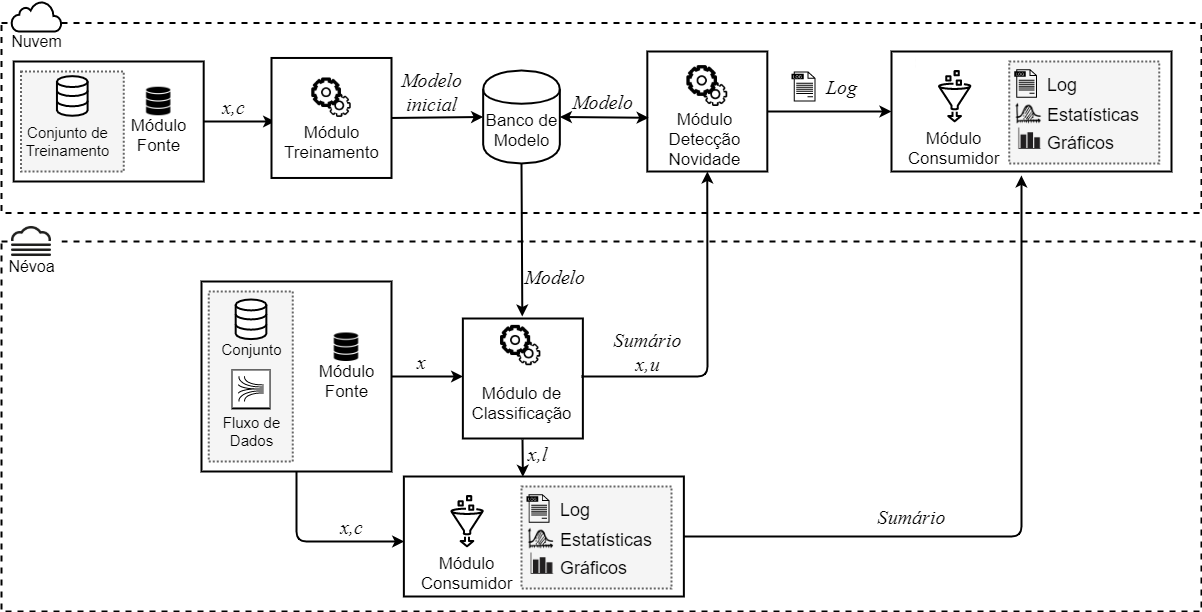
\includegraphics[width=\textwidth]{figuras/mfog-arch-v3_pt-br.png}
\caption{Arquitetura e fluxos de dados do \mfog.}
\label{fig:arch}
\end{figure}

A implementação do \mfog segue a arquitetura \arch formalizada por
\citeonline{Cassales2019a}, discutida na \refsec{cassales}.
A arquitetura \arch
% (e outras arquiteturas de NIDS)
estabelece que um serviço de
captura e tratamento de dados é instalado na borda de uma rede local com
dispositivos \iot.
Na presente implementação, esse serviço de captura e tratamento é representado
pelo \source.

O \source é dependente da fonte de dados, executando a transformação dos
formatos dos \datasets para um fluxo de exemplos (representado por $x$ na \reffig{arch})
compatível com o restante da implementação.
Além de fornecer exemplos tratados para o \classify, o \source também fornece
exemplos com a classe original (representado por $x,c$ na \reffig{arch})
\notafa{somente na fase de treinamento o source fornece exemplos rotulados par ao sink, certo?}
\hlfa{para o \sink e para o \offline}.

O \sink é responsável por agregar todos resultados do \mfog e,
juntamente com os valores do \dataset fornecidos pelo \source, por computar
as métricas de qualidade de classificação.
Além disso, esse módulo também coleta e agrega métricas base para as avaliação de
escalabilidade e métricas de uso de recursos computacionais.

Os dados resultantes do serviço de captura e tratamento (representado no \mfog
pelo \source) são ingeridos pela aplicação no \classify. A ingestão é feita por
meio de um operador fonte, fornecida pela plataforma \flink.
% \notake{TCP e apache flink}
% conexão TCP (\emph{Transmission Control Protocol}).
Na plataforma, com o modelo de classificação disponível, os exemplos são
classificados seguindo o algoritmo MINAS original discutido na \refsec{minas-og}.
A etiqueta atribuída pela classificação, ou meta-etiqueta de desconhecido,
juntamente com o exemplo original (representado por $x,l$ na \reffig{arch})
são enviados para o \sink.
Além disso, se o exemplo não for classificado, o exemplo e a meta-etiqueta de
desconhecido (representado por $x,u$ na \reffig{arch}) são enviados para o
\detector.
\notahl{processaa ND em paralelo?}
Outra comunicação é o envio das modificações ao sumário estatístico do modelo de
classificação (representado por $Summary$ na \reffig{arch}) do \classify para o
\detector.

O \detector é responsável por executar o processo de detecção de novidade,
atualizando o modelo de classificação, e entregar o novo modelo às instâncias do
\classify, através do serviço de armazenamento de modelo (\emph{Model Store} na
\reffig{arch}).
O \detector também envia meta-informações sobre o processo de detecção de
novidade (representado por $Log$ na \reffig{arch}) para o \sink.

% \nota{
% nao seria legal fazer um diagrama pq ai vc pode usar ate nos slides de como eh
% essa implementacao. Faz no draw io pra que de pra usar na monografia e de para
% enxergar na apresentacao
% }

O \mfog utiliza em seus módulos a distribuição oferecida pela plataforma \flink
como paralelização, ou seja, utiliza uma instância de trabalho (\emph{job}) por
dispositivo de classificação, sendo que cada instância de trabalho aloca um
gerenciador de tarefas por processador.
Dessa forma, busca-se a escalabilidade no ambiente de \fog para o \classify.
O \offline, por ser utilizado somente uma vez para gerar o modelo
de classificação inicial, não tem impacto na escalabilidade geral do sistema.
O \detector também é implementado na plataforma \flink e, por ser hospedado em
ambiente de \cloud, herda as qualidades desse ambiente incluindo escalabilidade.
\notake{destaque sentença}
O restante do sistema (\source, \sink, armazenamento de modelo) não é foco deste
estudo e sua escalabilidade, desde que não afete a escalabilidade do \classify e
\detector.
\notahl{Questões que precisam ser tratadas:\\
- Paralelização da classificação: como agrupar os dados e dividir o processamento?\\
- ND: como saber o que agrupar (dos nós) e como dividir?
Padrões podem ser locais? Ou sempre se aplicam a todos os nós?}
\notafa{frase incompleta}

% ------------------------------------------------------------------------------
\section{Metodologia de Avaliação}\label{sec:esperados}

% \nota{reestrutura 2:
%   A - cenario
%   B - metodologia (como, o que vai implementar [kafka, python, flink], como avaliar)
%   C - métricas (escalabilidade, qualidade)
%   D - resultados preliminares (python/kafka, flink)
% }

A avaliação da proposta apresentada é feita por meio de métricas extraídas da
literatura, divididas em duas partes: métricas de qualidade de classificação
e métricas de escalabilidade.
Métricas tradicionais de qualidade de classificação estabelecidas por trabalhos
de aprendizado de máquina não são adequadas para avaliar detecção de novidades em
\streams sem tratamento inicial. Felizmente, o tratamento necessário é
estabelecido por \citeonline{Faria2013} e expandido por
\citeonline{DaSilva2018,DaSilva2018thesis,Costa2019,Costa2019thesis}.
Além do tratamento estabelecido, as métricas tradicionais não são calculadas
somente para o conjunto completo, e sim para cada exemplo classificado.
Portanto, as métricas têm como índice o instante ($n$ nas equações à seguir),
informando a posição do exemplo em relação ao fluxo.

O tratamento estabelecido das métricas de qualidade para \streamMining define
que as métricas sejam extraídas de uma matriz de erro de classificação
multi-classe $\mathbf{E}_n$ (\refequ{matrix}), adaptada para detecção de
novidade.
A matriz de erro é preenchida com o número de eventos da classe $c_i$ classificados com
etiqueta $l_j$ até o instante $n$.
A \refequ{classes} representa o conjunto de classes presentes nos eventos
do fluxo até o instante $n$ e a \refequ{labels} representa o conjunto
de etiquetas atribuídas pelo classificador a eventos até o mesmo instante.

\begin{align}
  % x_n &= classify_{n-1}(x_n)\\
  % e_{i, j} &= classify_{n-1}(x_n)\\
  \mathbf{C}_n &= \{ c_1, c_2, \cdots, c_M \}  \label{eq:classes} \\
  \mathbf{L}_n &= \{ l_1, l_2, \cdots, l_J \}  \label{eq:labels} \\
  \mathbf{E}_n &= \begin{pmatrix}
    e_{1,1} & e_{1,2} & \cdots & e_{1,J} \\
    e_{2,1} & e_{2,2} & \cdots & e_{2,J} \\
    \vdots  & \vdots  & \ddots & \vdots  \\
    e_{M,1} & e_{M,2} & \cdots & e_{M,J} 
  \end{pmatrix}  \label{eq:matrix}
\end{align}

As métricas de qualidade de classificação selecionadas para avaliar a
implementação do \mfog serão
taxa de desconhecidos ($UnkR$ na \refequ{unkr}) \cite{Faria2013},
acurácia média ($acc$ na \refequ{acc})
e Macro F-score ($Fscore$ na \refequ{fscore}, também referido na literatura por
F1M) \cite{Sokolova2009,DaSilva2018thesis}.
As métricas são extraídas para todos os exemplos classificados (instantes $n$)
da respectiva matriz de erro $\mathbf{E}_n$.

% \nota{'para todos os instantes n' ??}

% \nota{Explicar o que significa cada elemento nas fórmulas}

\begin{align}
  \mathit{UnkR}_n       &= \frac{1}{M} \sum_{i=1}^{M} \frac{\#Unk_i}{\#ExC_i} \label{eq:unkr} \\
  \mathit{acc}_n        &= \frac{1}{M} \sum_{i=1}^{M} \frac{tp_i + tn_i}{tp_i+fn_i+fp_i+tn_i}
  = \frac{1}{M} \sum_{i=1}^{M} \frac{\#Acc_i}{\#ExC_i}  \label{eq:acc} \\
  \mathit{Precision}_n  &= \frac{1}{M} \sum_{i=1}^{M} \frac{tp_i}{tp_i+fp_i} \\
  \mathit{Recall}_n     &= \frac{1}{M} \sum_{i=1}^{M} \frac{tp_i}{tp_i+fn_i} \\
  \mathit{Fscore}\beta_n &= (\beta^2 +1) \cdot
  \frac{
  \mathit{Precision} \cdot \mathit{Recall}
  }{
    \beta^2 \cdot \mathit{Precision} +\mathit{Recall}
  }\\
  \mathit{Fscore}1_n   &= 2 \cdot \frac{
    \mathit{Precision} \cdot \mathit{Recall}
    }{
      \mathit{Precision} +\mathit{Recall}
    } \label{eq:fscore}
\end{align}
% = 2 \cdot \frac{tp}{2 \cdot tp + fn + fp}
% \mathcal{L}         &= \frac{-1}{N} \sum_{i=1}^{M} \sum_{j=1}^{J} y_{i,j} \log(p_{i,j})

% \nota{usar coeficiente d-intra vs d-extra grupo para determinar K de
% cada label. Também pode-se usar os mesmos coeficientes para _log_}

A transformação do fluxo de saída em uma matriz de erro é realizada no \sink,
\notahl{como tratar o paralelismo desse elemento?\\
Ele dá conta de todo o fluxo recebido dos classificadores?}
\hlhl{onde} 
\hlhl{tem-se disponível o fluxo original}
\hlhl{com as etiquetas corretas e o fluxo resultante}
\hlhl{da classificação.}
Esse módulo deve levar em consideração que pode haver reclassificação de um
evento, previamente rotulado como desconhecido, em padrões oriundos de classe
novidade ou extensão devido ao processo de detecção de novidades executado
posteriormente ao surgimento do padrão em questão.

% Portanto os resultados são computados em função do fluxo de saída, então os $n$ nas
% equações são o índice do evento de saída.
% $\mathbf{unk}$ é o conjunto de eventos marcados como desconhecidos.
% \nota{oque eh unk? nesse paragrafo acima, erro de compilacao do latex?}

% \nota{frase confusa, eh so tirar o COMO e quebrar a frase: Esse módulo deve levar em consideração que
% COMO pode haver reclassificação de um evento, previamente rotulado como
% desconhecido, em padrões oriundos de classe novidade ou extensão devido ao
% processo de detecção de novidades executado posteriormente ao surgimento
% do padrão em questão}

% \begin{align}
%   E_{n,i,j} &= \bordermatrix{~ & c_i & \neg c_i \cr
%   l_j       & TP = \alpha           & FP = \gamma - \alpha                 \cr
%   \neg l_j  & FN = \beta - \alpha   & TN = n - (\alpha + \beta + \gamma)  \cr} \\
%   FM1       &= \frac{TP}{TP+\frac{FP+FN}{2}}
% \end{align}

% Os valores da matriz de erro para 

% \begin{align}
%   \alpha _j &= max( \{ |e_{i,j}|: i = 1 .. I \wedge \in \mathbf{E}_n \})
%           & \text{máximo da linha (etiqueta)} \\
%   a_j &= i: |e_{i,j}| = \alpha _j
%           & \text{índice da classe associada à etiqueta} \\
%   \beta   &= \sum_{j = 0}^{J} e_{i,j} : e_{i,j} \in \mathbf{E}_n
%           & \text{soma de uma coluna (etiqueta)} \\
%   \gamma  &= \sum_{i = 0}^{I} a_{i,j} : e_{i,j} \in \mathbf{E}_n
%           & \text{soma de uma linha (classe)}
% \end{align}

As métricas de escalabilidade selecionadas são: número de nós processadores,
tipo de processadores, uso de memória, tempo de processamento, taxa de eventos
processados e latência entre a produção e classificação de um evento.

% \begin{align}
%   \Delta { } t_n       &= t_{n,sink} - t_{n,source} \label{eq:delta-t} \\
%   \overline{\Delta { } t}_n       &= \frac{1}{N} \sum_{i=1}^{N} \Delta { } t_n  \label{eq:avg-delta-t} \\
%   \alpha &= \# processors \\
%   \gamma &= \frac{\overline{\Delta { } t}}{}
% \end{align}

% \nota{
% como assim os resultados sao validos so se tiverem essas metricas? Entao quer
% dizer que qual medida eh valida? Vc quis dizer que se as medicoes que vc extrair
% com essas metricas forem iguais as medicoes do minas original, entao ai eh
% valido. Eh Isso?
% }

Da implementação do \mfog é prevista a execução de experimentos com \datasets
diversos, em especial os \datasets reais como \emph{Kyoto 2006+},
que contenham evolução de conceitos.
Os resultados desses experimentos irão conter as seguintes métricas:

\begin{enumerate}[label={\alph*)}]
  \item Qualidade de classificação (taxa de desconhecidos, F1M);
  \item Escalabilidade (número de processadores, volume processado, tempo
  decorrido);
  \item Recursos computacionais utilizados (memória, tempo de processamento,
  operações de leitura e escrita).
\end{enumerate}

Para a validação da corretude da implementação do \mfog com relação ao algoritmo
MINAS original, as métricas de qualidade de classificação serão extraídas de
ambas as Implementação e comparadas.

% !TeX root = ./00.ppgcc-2020.tex

% \chapter{Implementação}\label{cha:implementacao}

% % procedimento experimental previamente definido de ambos, \mfog e da
% % implementação original do algoritmo MINAS, e comparadas.

% % !TeX root = ./00.ppgcc-2020.tex

\subsection{Implementações Preliminares}\label{sec:resultados}

No desenvolvimento parcial desta pesquisa, algumas experimentações e algumas
ferramentas de teste já foram desenvolvidas.
Aspectos desses desenvolvimentos são descritos a seguir.
% obrigado hélio.

\subsubsection{Implementação com \python e \kafka}

A primeira implementação e avaliação do \mfog realizada foi construída sobre a
linguagem \python com o sistema de fila de mensagens \kafka e a respectiva
biblioteca de conexão.
A escolha desse conjunto para a implementação ocorreu \hlhl{devido à ampla}
disponibilidade de bibliotecas de aprendizagem de máquina no ecossistema
\python e, à simplicidade geral da linguagem.
Na implementação desenvolvida, o sistema \kafka recebe mensagens e as armazena
em tópicos distribuídos em partições replicadas em nós de um \cluster,
gerenciados por um nó mestre e suportados pelo serviço de gerenciamento de
configuração distribuída \emph{Apache ZooKeeper}.
A aplicação \emph{Python} consome eventos através da interface \emph{Consumer API},
que expõe a distribuição através da associação de um consumidor às partições
mantidas pelo \kafka.

Para essa implementação, havia a hipótese de que a distribuição de
mensagens gerenciada pelo \kafka
se estenderia a processos consumidores, efetivamente distribuindo o volume de
mensagens entre eles igualmente.
No entanto, a hipótese foi refutada nos experimentos realizados.
Os experimentos em questão foram compostos de 8 processos consumidores, um
processo produtor, uma instância \kafka com 8 partições em seu tópico principal
e uma instância \emph{Apache ZooKeeper} associada à instância \kafka.
% A hipótese era que, como o número de partições igualava o número de consumidores,
% cada consumidor associaria-se a uma partição, distribuindo os dados igualmente
% entre os consumidores para a paralelização a execução.
A hipótese foi refutada quando observou-se que o número de
mensagens consumidas por um dos 8 processos representava a maioria (mais de
80\%) do volume introduzido no sistema, o restante sendo distribuído entre
outros 3 processos e o restante dos processos não recebia nenhuma mensagem.
Portanto, a iniciativa de implementar o algoritmo MINAS em \python com \kafka e
atingir os objetivos de distribuição falhou, o que levou à reconsideração das
plataformas escolhidas.

\subsubsection{Implementação com \flink}

% \nota{citar ferramentas e a escolha só depois do python e kafka}
% \nota{entre flink e spark, outro grupo de pesquisa já está explorando spark}

A segunda alternativa explorada teve por inspiração o trabalho de
\citeonline{Viegas2019} e, como outro grupo de pesquisa já estava explorando
o algoritmo na plataforma \emph{Apache Spark}, a segunda implementação
foi baseada na plataforma \flink.

A plataforma \flink tem modelos de processamento tanto de fluxos como em lotes.
O modelo em lotes é implementado como extensão do modelo de fluxos e, apesar
de não ser foco desse trabalho, mostrou-se útil para a construção do \offline,
já que o conjunto consumido por esse módulo é limitado.

Um desafio encontrado durante o desenvolvimento da implementação do \mfog foi a falta
de bibliotecas na plataforma \flink que disponibilizem versões adaptadas
à plataforma de algoritmos base para o algoritmo MINAS.
Em especial, a ausência dos algoritmos \emph{K-means} e \emph{CluStream}
gerou carga imprevista sobre o processo de desenvolvimento
resultando no atraso do processo de desenvolvimento.

Esta implementação segue a arquitetura descrita na \refsec{descricao} e as
avaliações e resultados esperados descritos neste \refcap{proposta}
referem-se à implementação do \mfog na plataforma \flink.

% % !TeX root = ./00.ppgcc-2020.tex

\section{Implementação com MPI}

The original MINAS algorithm has a companion unpublished implementation (\refminas)
written in Java using MOA library base algorithms such as K-means and CluStream,
but our implementation only used K-means.
Another difference between \refminas and \mfog is the calculus of the cluster radius 
from the distances of elements forming the cluster and the cluster's center.
\refminas uses the maximum distance while \mfog uses the standard deviation
of all distances as described in \cite{Faria2016minas}.

\newcommand{\val}{$\vec{v}\,$\xspace}
The stream formats for input and output are also of note.
As input, the algorithm takes samples (\val), which are a sequence of numbers
with dimension $d$.
In addition to \val, for both training and evaluation, the class
identifier is provided as a single character, along with a unique item identifier
(\emph{uid}), which can otherwise be determined from the sample index in the stream.

As its output, the algorithm returns the original sample \val followed by the
assigned label. Adjustments can easily be made to provide the output results as
a tuple containing \emph{uid} and the assigned label.

% - Reprocessamento dos exemplos utilizados para atualização do modelo:
%   - Muda o comportamento do operador de fluxo de `Map` para `Flatmap`, ou seja,
%     requer outro fluxo de saída para a transmissão de padrões novidade (alarmes);
%   - Para reclassificação a definição de raio é modificada de `r = f * σ` (fator
%     multiplicando desvio padrão) para `r = max(distance)` (distância máxima);
%   - Passível da crítica de *overfitting*. Isto é, este processo pode
%     inflar a métrica de precisão;
%   - **Solução:** *em aberto*;


\begin{algorithm}[htb]
% {\scriptsize
% \begin{multicols}{2}
    % \SetAlgoVlined
    \SetKwProg{Function}{Function}{:}{}
    \SetKwFor{With}{with}{}{}
    \SetKw{continue}{continue}
    % 
    \SetKwData{MEPC}{MEPC}
    \SetKwData{NF}{NF}
    \SetKwData{mpiSize}{mpiSize}
    \SetKwData{mpiRank}{mpiRank}
    \SetKwData{EndOfStream}{EndOfStream}
    % 
    \SetKwInOut{KwParams}{Parameters}
    \KwParams{mpiNodeRank as \mpiRank}
    % 
    \SetKwFunction{Mfog}{Mfog}
    \SetKwFunction{Sampler}{Sampler}
    \SetKwFunction{Classifier}{Classifier}
    \SetKwFunction{Detector}{Detector}
    \SetKwFunction{modelReceiver}{modelReceiver}
    % 
    \SetKwFunction{typeOf}{typeOf}
    % 
    \SetKwFunction{Thread}{Thread}
    \SetKwFunction{Lock}{Lock}
    \SetKwFunction{readLock}{readLock}
    \SetKwFunction{writeLock}{writeLock}
    % 
    \SetKwFunction{receive}{receive}
    \SetKwFunction{send}{send}
    \SetKwFunction{broadcast}{broadcast}
    % 
    \SetKwFunction{nearestCluster}{nearestCluster}
    \SetKwFunction{NoveltyDetection}{NoveltyDetection}
    \SetKwFunction{handleModelSleep}{handleModelSleep}
    \SetKwFunction{removeOldSamples}{removeOldSamples}
    \SetKwFunction{now}{now}
    % 
    \KwIn{ModelSet, Sample Stream}
    % \KwOut{Classified Stream as $out$}
    % 
    \Function{\Mfog{ModelStream, InputStream, OutputStream}}{
        ModelSet = $\emptyset$\;
        ModelSetLock = \textbf{new} \Lock()\;
        \eIf(\emph{root}){\mpiRank == 0}{
            \textbf{new} \Thread(\Detector, [OutputStream, ModelSet, ModelSetLock])\;
            \Sampler(InputStream, ModelSet, ModelSetLock)\;
        }(\emph{leaf}){
            \textbf{new} \Thread(\modelReceiver, [ModelSet, ModelSetLock])\;
            \Classifier(ModelSet, ModelSetLock)\;
        }
    }
\caption{MFOG: main MPI entry-point.}
\label{alg:MFOG}
\end{algorithm}

\begin{algorithm}[htb]
    \SetKwFor{With}{with}{}{}
    \SetKw{continue}{continue}
    % 
    \SetKwData{MEPC}{MEPC}
    \SetKwData{NF}{NF}
    \SetKwData{mpiSize}{mpiSize}
    \SetKwData{mpiRank}{mpiRank}
    \SetKwData{EndOfStream}{EndOfStream}
    % 
    \SetKwProg{Function}{Function}{:}{}
    \Function{\Classifier{ModelSet, ModelSetLock}}{
        \While{ True }{
            sampe = \receive(SampleType, root)\;
            \lIf{sample == \EndOfStream}{\textbf{break}}
            sample.label = unknown\;
            \With{\readLock(ModelSetLock)}{
                (distance, cluster) = \nearestCluster(sample, ModelSet)\;
            }
            \If{distance $<$ cluster.radius}{
                sample.label = cluster.label\;
            }
            \send(root, SampleType, sample)\;
        }
    }
%     \label{alg:MFOG-classifier}
%     \caption{MFOG: Classifier task.}
% \end{algorithm}
% \begin{algorithm}
    % \SetKwProg{algorithm}{algorithm}{:}{}
    \SetKwFor{With}{with}{}{}
    \SetKw{continue}{continue}
    % 
    \SetKwData{MEPC}{MEPC}
    \SetKwData{NF}{NF}
    \SetKwData{mpiSize}{mpiSize}
    \SetKwData{mpiRank}{mpiRank}
    \SetKwData{EndOfStream}{EndOfStream}
    % 
    \SetKwProg{Function}{Function}{:}{}
    \Function{\modelReceiver{ModelSet, ModelSetLock}}{
        \While{ True }{
            cl = \receive(ClusterType, root)\;
            \lIf{cl == \EndOfStream}{\textbf{break}}
            \With{writeLock(ModelSetLock)}{
                ModelSet = ModelSet $\cup$ cl\;
            }
        }
    }
    % \label{alg:MFOG-model}
    % \caption{MFOG: model receiver task.}
\caption{MFOG Leaf Tasks: Model Receiver and Classifier.}
\label{alg:MFOG-leaf}
\end{algorithm}
\begin{algorithm}[htb]
    \SetKwFor{With}{with}{}{}
    \SetKw{continue}{continue}
    % 
    \SetKwData{MEPC}{MEPC}
    \SetKwData{NF}{NF}
    \SetKwData{mpiSize}{mpiSize}
    \SetKwData{mpiRank}{mpiRank}
    \SetKwData{EndOfStream}{EndOfStream}
    \SetKwInOut{KwParams}{Parameters}
    \KwParams{mpiClusterSize as \mpiSize}
    \SetKwProg{Function}{Function}{:}{}
    \Function{\Sampler{InputStream, ModelSet, ModelSetLock}}{
        % ModelSet = read()\;
        % broadcast(ModelSet)\;
        dest = 1\;
        \ForEach{ sample from InputStream }{
            \If{\typeOf(sample) is Cluster}{
                \broadcast(ClusterType, sample, root)\;
                \With{\writeLock(ModelSetLock)}{
                    ModelSet = ModelSet $\cup$ sample\;
                }
                \continue\;
            }
            % sample.label = unknown\;
            \send(dest, SampleType, sample)\;
            dest = dest $+ 1$\;
            \lIf{dest $>$ \mpiSize}{dest = 1}
        }
    }

%     \label{alg:MFOG-sampler}
%     \caption{MFOG: sampler Module.}
% \end{algorithm}
% \begin{algorithm}
    \SetKwProg{algorithm}{algorithm}{:}{}
    \SetKwFor{With}{with}{}{}
    \SetKw{continue}{continue}
    % 
    \SetKwData{cleaningWindow}{cleaningWindow}
    \SetKwFunction{removeOldSamples}{removeOldSamples}
    \SetKwData{noveltyDetectionTrigger}{noveltyDetectionTrigger}
    \SetKwData{MEPC}{MEPC}
    \SetKwData{NF}{NF}
    \SetKwData{mpiSize}{mpiSize}
    \SetKwData{mpiRank}{mpiRank}
    \SetKwData{EndOfStream}{EndOfStream}

    \KwParams{\cleaningWindow, \noveltyDetectionTrigger}

    \SetKwProg{Function}{Function}{:}{}
    \Function{\Detector{OutputStream, ModelSet, ModelSetLock}}{
        lastCleanup $\leftarrow 0$\;
        \While{ True }{
            sampe = \receive(SampleType, any)\;
            \lIf{sample == \EndOfStream}{\textbf{break}}
            % $out \leftarrow$ sample\;
            OutputStream.append(sample)\;
            \If{sample.label == unknown}{
                UnknownSet = UnknownSet $\cup$ sample\;
                \If{$|\;UnknownSet\;| \geq$ \noveltyDetectionTrigger}{
                    novelties = \NoveltyDetection(ModelSet, *UnknownSet)\;
                    \With{\writeLock(ModelSetLock)}{
                        ModelSet = ModelSet $\cup$ novelties\;
                    }
                    \ForEach{ cl in novelties }{
                        \broadcast(ClusterType, cl, root)\;
                    }
                }
                \If{ sampe.uid $ > $ ( lastCleanup $ + $ \cleaningWindow )}{
                    UnknownSet $\leftarrow$ \removeOldSamples(UnknownSet, lastCleanup)\;
                    lastCleanup $ \leftarrow $ sampe.uid\;
                }
            }
        }
    }
    % \label{alg:MFOG-detector}
    % \caption{MFOG: detector task.}
\caption{MFOG Root Tasks: Sampler and Detector.}
\label{alg:MFOG-root}
\end{algorithm}

For evaluation purposes, an \mfog implementation was made using MPI (\emph{Open
MPI 4.0.4}).
The program is organized in a single program multiple data (SPMD)
programming model, so a single version of the \mfog program was initiated on all
nodes, being that one of them would perform the root role, while the others ran
as leaves, the program entry point is illustrated on Algorithm \ref{alg:MFOG}.
On the root process, a sampler thread is responsible for distributing the
sampled flow information (\val) to the classifier nodes, using a round-robin
load balancing scheme.
The other thread on the root process is responsible for receiving the
classification results and for processing the unknown samples in the search for
novelties.
The root process functions are illustrated in Algorithm \ref{alg:MFOG-root}.
Each leaf node runs a model adjustment thread and multiple (up to the number of
cores) classifier threads. The leaf tasks are illustrated in Algorithm
\ref{alg:MFOG-leaf}.
The overall sequence of interactions is shown in Figure \ref{fig:mfog-mpi-life}.

\begin{figure}[htb]
  \centerline{
    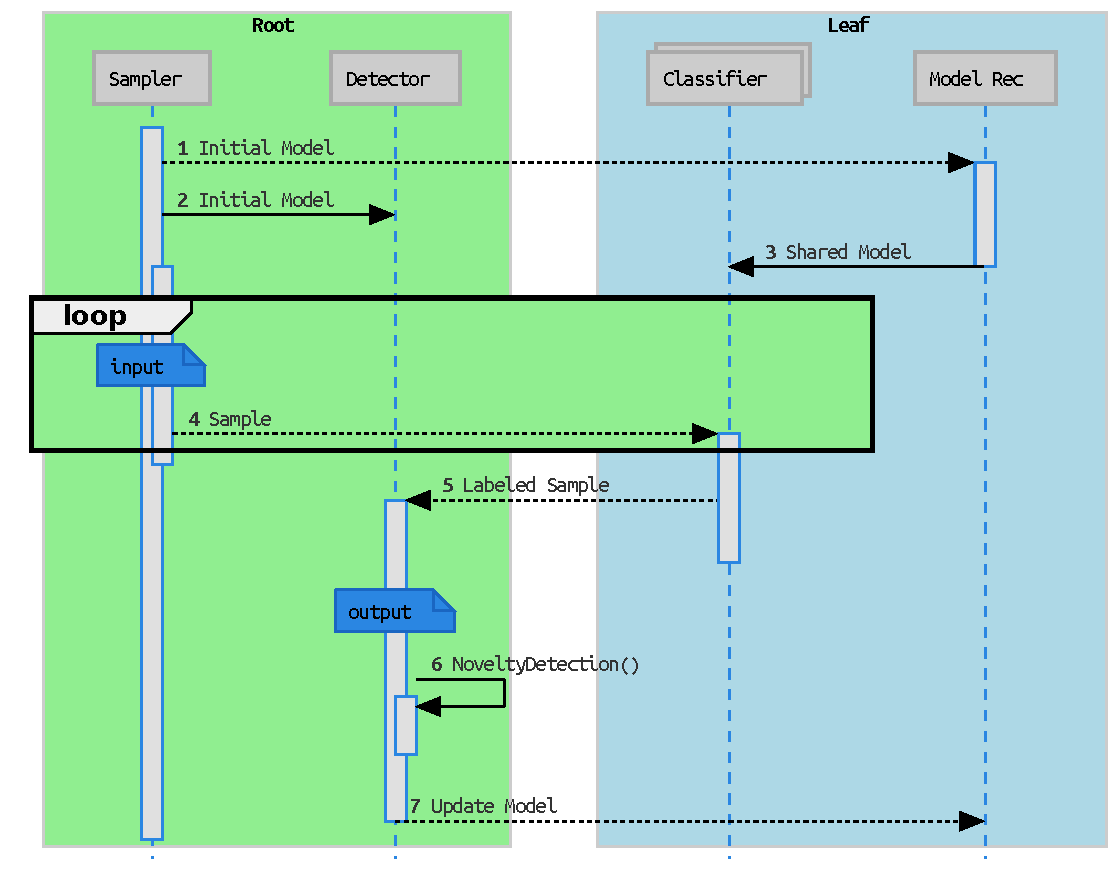
\includegraphics[width=0.75\linewidth,page=1]{figures/lifecycle-uml-svg.pdf}
  }
  \caption{\mfog life line overview.}
  \label{fig:mfog-mpi-life}
\end{figure}


\chapter{Experimentos e Resultados}\label{cha:results}

Este capítulo apresenta o ambiente experimental e os resultados obtidos dos
experimentos, discutindo as métricas de qualidade da classificação e
escalabilidade do \mfog.

% !TeX root = ./00.ppgcc-2020.tex

\section{Ambiente de Teste}\label{sec:ambiente}

Com o objetivo de avaliar esta proposta e averiguar os efeitos da distribuição
da detecção de novidades em um cenário \iot, construiu-se um ambiente
experimental de névoa.

Este ambiente é composto por três computadores de única placa (\emph{Single
Board Computer}) modelo Raspberry Pi 3 model B, equipados com o SoC
(\emph{system-on-chip} - sistema em um chip) de arquitetura ARM \emph{BCM2837} com
$4$ núcleos de processamento à frequência de $1.2\,GHz$, $32\,kB$ e $512\,kB$ de
memória \emph{cache} nível 1 e 2 respectivamente, $1\,GB$ de memória RAM,
armazenamento em cartão SD e conectados por rede cabeada \emph{Ethernet}.
% Switch
% Hélio:
%    Há algo estranho na descrição dos nós; parece que você está misturando nós e cores.
%    Talvez seja mais claro falar do número de nós, ao invés dos cores...
% ficou melhor!

A ideia central é criar um cluster simples simulando \emph{gateway} de uma rede
\iot com recursos limitados.
Este cluster armazenou todo o código-fonte, binários (compilados no mesmo cluster) e
\dataset.
Nesta configuração, o \dataset é armazenado no cartão SD do nó raiz e é lido para
cada execução do experimento.
Todos os experimentos foram executados neste cluster para isolamento de outras
variações imprevistas e para garantir que as comparações seriam justas com
\emph{software} e \emph{hardware} constante.

% The idea was to create a simple cluster simulating an \iot network with
% constrained resources at the edge of the network.
% This cluster stored all source code, binaries (compiled and linked in place) and
% data sets.
% In our setup, the data set is stored in the root's node SD card and is read for
% each experiment.
% All experiments were executed in this cluster for isolation of otherwise
% unforeseen variations and for safe software comparison with constant hardware.
% data sets, being accessed via our laboratory network over Secure Shell (SSH).

O \dataset \emph{Kyoto 2006+}\footnote{Disponível em
\url{http://www.takakura.com/Kyoto\_data/}.}, tráfego das \emph{Honeypots} da
Universidade de Kyoto, é a referência de um cenário real para este trabalho.
% será que é o ``foco''? Talvez é a ``referência de um cenário real''...(?)
Este \dataset contém dados ainda representativos (até 2015) e as característica
desejáveis de um conjunto de dados (realismo, validade, etiquetas previamente
definidas, alta variabilidade, reprodutibilidade e disponibilidade pública) são
atendidas \cite{KyotoDataset,Song2011kyoto}.

O segmento utilizado deste \dataset é o de Dezembro de 2015, contendo $7\:865\:245$ instâncias.
Deste segmento, são mantidas apenas instâncias associadas a tráfego normal ou
a ataques conhecidos, identificados por \nids que tenham mais de $10\,000$ instâncias
para significância, como feito previamente por \citeonline{Cassales2019}.
% , this removes 46,390 instances. TODO: revisar, pois 7M != 700K.
As instâncias mantidas são normalizadas para que o valor de cada característica
original (como endereço IP, duração do fluxo, serviço) seja transposta para o
intervalo Real $[0, 1]$.

O conjunto resultante da operação recém descrita é então dividido em dois
conjuntos, treinamento e teste.
Para avaliar a detecção de ataques, o conjunto treinamento é composto apenas de
tráfego normal, contendo $72\:000$ instâncias.
O conjunto de teste possui $653\:457$ instâncias, sendo elas
$206\:278$ instâncias com classe ``$N$'' (normal) e
$447\:179$ instâncias com classe ``$A$'' (ataque).
%
% Não entendi essa questão de filtrar apenas os ``normal'' class no training set... Hélio
% acho que fez sentido... detectar o que não se aproxima de normal como novidade...

Destaca-se que essa manipulação do \dataset causa \emph{Overfitting} para a classe
normal e \emph{under-fitting} para a classe ataque, pois o sistema primeiro
precisa detectar um padrão novidade para então adicionar ao modelo.
%O foco deste trabalho não é a otimização da detecção de intrusão é contexto de validar metodologia de construcao do \mfog - distribuição e paralelismo em ambiente em \fog.
Como o foco deste trabalho é na arquitetura e metodologia de paralelização e
distribuição em névoa, a otimização do processo de detecção de intrusão não foi
abordada, deixando a questão de escolha do \dataset e do processo de sua manipulação
 em aberto.

Quanto aos parâmetros do algoritmo \minas, ilustrados na Figura
\ref{fig:params}, os valores foram escolhidos por \hlke{serem valores comuns para o
algoritmo presentes na literatura} \cite{Faria2013Minas,Faria2016minas} e na
implementação de referência \refminas \cite{Faria2013source}.
Os parâmetros que não tem valores comuns na literatura foram escolhidos e ajustados até os
os resultados obtidos se aproximarem aos resultados da implementação de referência \refminas.

\begin{figure}[htb]
  \centering
  \begin{lstlisting}
    MinasParams minasParams = {
      .k=100, .dim=22, .precision=1.0e-08,
      .radiusF=0.25, .minExamplesPerCluster=20, .noveltyF=1.4,
      .thresholdForgettingPast = 10000,
    };
  \end{lstlisting}
  \caption{Parâmetros do algoritmo \minas.}
  \label{fig:params}
\end{figure}

Os parâmetros utilizados da literatura são
\texttt{k}, que é o número de \mclusters gerados pelo algoritmo de agrupamento,
\texttt{minExamplesPerCluster}, que indica o número mínimo de exemplos para um
\mcluster válido (representatividade) e,
\texttt{thresholdForgettingPast}, que estabelece o limite para remoção de exemplos do conjunto de
desconhecidos.

Os parâmetros escolhidos por aproximação de resultados são:
\texttt{precision}, que é o valor limite para melhora na distância global reduzindo as 
iterações no algoritmo de agrupamento (otimização),
\texttt{radiusF}, que corresponde ao fator que multiplica o desvio padrão das distâncias entre o
centro e cada exemplo formador do novo \mcluster definindo o raio do \mcluster
e,
\texttt{noveltyF}, que é o fator que multiplica o desvio padrão das distâncias do
\mcluster mais próximo distinguindo um novo padrão entre extensão e novidade.

% (k, minExamplesPerCluster, noveltyF, thresholdForgettingPast)
% (precision, radiusF)

% Para realização dos experimentos, diversas configurações de ambientes são
% propostas.
% Os ambientes selecionados são: local, 
% \notahl{o que muda na paralelização e na \textbf{distribuição} de instâncias
% do módulo \textbf{classificador}?}
% \hlhl{nuvem e névoa}.
% As configurações consistem na distribuição de módulos da implementação \mfog
% sendo executadas em combinações de ambientes nuvem e névoa com variada
% quantidade de nós.
  % dá-lhe Yoda! Hélio

% O ambiente local é composto por um único nó computacional, consistindo de um
% computador pessoal equipado com um processador de 8 núcleos, $16GB$ de memória e
% armazenamento em estado sólido (SSD) usado para o desenvolvimento e referência
% em comparações.
% O ambiente nuvem é provido pela utilização da infraestrutura de nuvem da
% Universidade Federal de São Carlos (Cloud{@}UFSCar\footnote{Disponível em
% \url{http://portalcloud.ufscar.br/servicos}}).
% O ambiente de névoa (\fog) é composto por computadores de única placa
% (\emph{Single Board Computer}) equipados com processador de arquitetura ARM de 4
% núcleos, $1GB$ de memória, armazenamento em cartão SD (\emph{SD-card}) e
% conectados por rede sem fio.

% A combinação de diferentes formas de distribuição dos nós tem por objetivo \hlhl{demonstrar padrões de
% latência} e qualidade que podem afetar implantações em ambientes reais que não
% são geralmente destacados quando os experimentos são realizados em um único
% nó ou ambiente.

% Faz parte também do ambiente de teste os conjuntos de dados (\datasets)
% \emph{KDD99}
% % \hlfa{e \emph{Kyoto 2006+}}
% e \emph{Kyoto 2006+}
% que foram selecionados por motivos distintos.

% O \dataset \emph{Kyoto 2006+} é o foco deste trabalho, pois contém dados ainda
% representativos (até 2015) e as característica desejáveis de um conjunto de
% dados (realismo, validade, etiquetas previamente definidas, alta variabilidade,
% reprodutibilidade e disponibilidade pública) são atendidas
% \cite{KyotoDataset,Song2011kyoto}.

% O \dataset \emph{KDD99} é amplamente utilizado em trabalhos de detecção de
% anomalia.
% Porém, como não possui mais a característica de realismo, uma vez que foi
% construído em 1998, neste trabalho o \dataset \emph{KDD99} é utilizado somente
% para que o leitor possa comparar com outros trabalhos
% \cite{Tavallaee2009,Protic2018KddKyoto}.

% Os dois \datasets mencionados e outros abordados em discussão e avaliados como
% relevantes são

% Por exemplo, o KDD original tem 41 atributos. A base é rotulada para 24
% tipos de ataques divididos em 4 grupos: DOS ...
% 
% O paper que analisou a fundo o KDD99 foi este: 
% 
% M. Tavallaee, E. Bagheri, W. Lu, and A. Ghorbani, “A detailed analysis
% of the KDD Cup 1999 data set,” in Proc. 2nd IEEE Symp. Comput. Intell.
% Secur. Defense Appl., 2009, pp. 1–6.
% 
% Qual é o defeito dele? tem muitos dados replicdos tanto na base de
% treinamento quento na de teste, o que gera viés nos resultados. Para
% resolver isso propuseram o NSL-KDD que é um subconjunto do KDD que evita
% esse problema

% \notake{
%   CICIDS2017 {https://www.unb.ca/cic/datasets/ids-2017.html} e
%   ISCXTor2016 {https://github.com/ahlashkari/CICFlowMeter}
% }
% \notafa{Uma sugestão seria usar datasets artificiais também a fim de avaliar
% outras caracteristicas tais como: nro de atributos, frequencia do surgimento de
% novidades, mudanças abruptas, graduais, etc. }
% \begin{table}[ht]
%   \caption{Sumário dos conjuntos de dados}
%   \centering
%   \begin{scriptsize}
%   \begin{tabularx}{\linewidth}{X|X|X|X}
%     Nome &
%       Origem &
%       Descrição &
%       Acesso Público \\
%     \hline
%     \hline
%     \emph{KDD99} \cite{Tavallaee2009,Protic2018KddKyoto} &
%       Captura de Fluxos de rede com ataques simulados &
%       41 atributos (sumário de fluxo), 23 classes, $4\;898\;431$ instâncias, $709$ MB &
%       \url{https://kdd.ics.uci.edu/databases/kddcup99/kddcup99.html} \\
%     \hline
%     \emph{Kyoto 2006+} \cite{Song2011kyoto,Protic2018KddKyoto}&
%       Captura de Fluxos de rede com HoneyPot &
%       23 atributos (sumário de fluxo), 3 classes, $7\;865\;245$ instâncias e $1.3$ GB (dez-2015) &
%       \url{https://www.takakura.com/Kyoto_data/new_data201704/} \\

%       %  0.000000 other 0 0 0 0.00 0.00 0.00 0 0 0.00 0.00 0.00 S0 00 0 -1
%       %  fdbd:f115:35b2:0424:40aa:098c:03e5:149b 3712
%       %  fdbd:f115:35b2:c891:7db9:2762:6182:03eb 445 00:00:00 tcp
    
%        \hline
%     % ISCXTor2016 \cite{Draper-Gil2016} &
%     %   Origem &
%     %   28 atributos,  &
%     %   \url{https://www.unb.ca/cic/datasets/tor.html} \\
%     % \hline
%     % ISCXVPN2016 \cite{Lashkari2017} &
%     %   Origem &
%     %   28 atributos,  &
%     %   \url{https://www.unb.ca/cic/datasets/tor.html} \\
%     % \hline
%     CICIDS2017 \cite{Sharafaldin2018cicids2017} &
%       Captura de Fluxos de rede com ataques simulados com perfil de trafego de 25
%       usuários normais e de 6 perfis de ataques durante 5 dias (1º dia sem ataque) &
%       80 atributos (sumário de fluxo extraído de CICFlowMeter), 15 classes,
%       $2\;830\;751$ instâncias e 1.2GB em arquivos \emph{pcap} e \emph{csv} &
%       \url{https://www.unb.ca/cic/datasets/ids-2017.html} \\
%     \hline
%     \emph{Radial Basis Function} (RBF) da biblioteca \emph{Massive Online Analysis} (MOA)
%     \emph{4CRE-V2} &
%       Sintético gerado por função RBF da biblioteca MOA com características de
%       mudança e evolução de conceito &
%       Atributos ($\mathbb{R}$), exemplos, classes, evoluções e mudanças configuráveis &
%       \url{https://sites.google.com/site/nonstationaryarchive/home} \\
%     \hline
%   \end{tabularx}
%   \label{tab:summary-dataset}
%   \end{scriptsize}
% \end{table}


% \input{54.experimentos.tex}

% \FloatBarrier
\section{Experimentos, Métricas e Visualizações}
\label{sec:experiments}
% acho que convém explicar as demais tabelas de resultados...

\newcommand{\expA}{\textit{a-Referência}\xspace}
\newcommand{\expB}{\textit{b-Sequencial}\xspace}
\newcommand{\expC}{\textit{c-Paralelo}\xspace}
\newcommand{\expD}{\textit{d-Distribuído}\xspace}

Seguindo as especificações de ambiente da Seção \ref{sec:ambiente}, cada
experimento consiste na execução de um dos programas ((a)\minas referência 2013
\cite{Faria2013source}, (b) implementação sequencial do \minas com a nova
biblioteca, (c) \mfog em um ou (d) três nós) com variação do parâmetro de paralelismo,
fornecendo um modelo inicial e \dataset de teste como fluxo de entrada e
capturando o fluxo de saída para e extração das métricas estabelecidas na Seção
\ref{sec:avaliacao}.
Destes experimentos, listados na Tabela \ref{tab:exp-list}, os seguintes
resultados são apresentados.

\begin{table}[htb]
  \centering
  % \setlength\tabcolsep{0.5em}
  \caption{Listagem dos principais experimentos.}
  \label{tab:exp-list}
  \begin{tabular}{p{0.17\textwidth}|p{0.27\textwidth}|p{0.47\textwidth}}
  \textbf{Experimento} & \textbf{Programa}                 & \textbf{Características} \\\hline
  \expA                & \minas referência 2013            & Raio é a distância máxima. \\\hline
  \expB                & \minas sequencial para validação  & 
    Raio é o desvio padrão das distâncias;
    Modelo único;
    Remoção de desconhecidos mais agressivo. \\\hline
  \expC                & \mfog 1 nó, 4 processadores       & 
    Classificadores paralelos;
    Detecção de novidade assíncrona. \\\hline
  \expD                & \mfog 3 nós, 12 processadores     &
    Mais processadores;
    Comunicação em rede.
  \end{tabular}
  \end{table}

\subsection{Validação do algoritmo}

Para validar a biblioteca de funções do \mfog que implementa o algoritmo \minas,
uma versão do Algoritmo \ref{alg:minas-main} foi construída, sem classificadores
paralelos ou detecção de novidade assíncrona, aspectos que caracterizam o \mfog.
Esta implementação utiliza a definição de raio da Equação \ref{eq:raio_paper}
(desvio padrão das distâncias).
Feita esta implementação foram realizados os experimentos \expB com esta
implementação e \expA com a implementação \minas referência.
Estes dois experimentos utilizam apenas um nó e um processador do ambiente
experimental, sendo que as métricas são extraídas conforme a \refsec{avaliacao}
e são comparadas nesta Subseção, mostrando a equivalência entre as implementações.

A Tabela \ref{tab:java-matrix} mostra a matriz de confusão no instante final do
fluxo de saída do experimento \expA.
Nesta matriz, o rótulo ``desconhecido'' é o caractere ``$-$'' e os valores de
associação e verdadeiro-positivo estão atrelados à coluna de cada rótulo; no
demais a matriz segue os atributos definidos na Seção \ref{sec:avaliacao}.
Esta matriz é comparada com a matriz de confusão do mesmo instante do fluxo de
saída do experimento \expB, e os resultados são apresentados na Tabela \ref{tab:libc-matrix}.

\begin{table}[hbt]%{\linewidth}
  {\footnotesize
  % \setlength\tabcolsep{0.5em}
  \begin{center}
  \caption{Experimento \expA, Matriz de confusão do \dataset \emph{Kyoto} Dez. 2015.}
  \label{tab:java-matrix}
  \begin{tabular}{l *{14}{|r} }
    Rótulos   &     - &       N &    1 &    2 &    3 &  4 &   5 &    6 &    7 &     8 &    9 &    10 &   11 &  12 \\\hline
    Classes  &       &         &      &      &      &    &     &      &      &       &      &       &      &     \\\hline
    \hline
    A        &  3\;774 &  438\;750 &  123 &  145 &  368 &  8 &  52 &  165 &    1 &  1\;046 &  161 &  2\;489 &   71 &  26 \\\hline
    N        &  8\;206 &  193\;030 &    0 &   79 &   44 &  0 &   0 &    0 &  229 &   181 &  154 &  4\;066 &  289 &   0 \\\hline
    \hline
    Associação &     - &       N &    A &    A &    A &  A &   A &    A &    N &     A &    A &     N &    N &   A \\\hline
    Hits ($tp$)     &     0 &  193\;030 &  123 &  145 &  368 &  8 &  52 &  165 &  229 &  1\;046 &  161 &  4\;066 &  289 &  26 
  \end{tabular}
\end{center}
}
\end{table}

Comparando as duas matrizes, a primeira diferença aparente é o índice do
primeiro rótulo novidade ($0$ ao invés de $1$), mas isso se deve apenas à decisão
arbitrária.
% A sentença a seguir está bem longa, difícil de acompanhar. Fragmentar?
A primeira diferença notável que influi nas métricas de qualidade é a falta de 3
rótulos novidade, $12$ rótulos no experimento \expA e $9$ no experimento \expB,
seguido do número de exemplos desconhecidos, $28\,567$ no experimento \expB e
$11\,980$ no experimento \expA e, o montante de exemplos incluídos nos rótulos
novidade, muito menor no experimento \expB.

\begin{table}[hbt]%{\linewidth}
  % {\small
  % \setlength\tabcolsep{0.5em}
  \begin{center}
  \caption{Experimento \expB, Matriz de confusão do \dataset \emph{Kyoto} Dez. 2015.}
  \label{tab:libc-matrix}
  \begin{tabular}{l|r|r|r|r|r|r|r|r|r|r|r}
    Rótulos &      - &       N &   0 &    1 &    2 &   4 &   5 &  6 &   7 &   8 &  10 \\\hline
    Classes  &        &         &     &      &      &     &     &    &     &     &     \\\hline
    \hline
    A        &  16\;086 &  429\;765 &  94 &  995 &  104 &   0 &  23 &  3 &  29 &  46 &  34 \\\hline
    N        &  12\;481 &  193\;642 &   3 &   94 &    0 &  47 &   0 &  0 &   0 &  11 &   0 \\\hline
    \hline
    Associação &      - &       N &   A &    A &    A &   N &   A &  A &   A &   A &   A \\\hline
    Hits ($tp$)     &      0 &  193\;642 &  94 &  995 &  104 &  47 &  23 &  3 &  29 &  46 &  34 
  \end{tabular}
  \end{center}
  % }
\end{table}

Estas três diferenças são atribuídas à divergência entre as definições de raio
discutidas na Seção \ref{sec:minas-og}, Equações \ref{eq:raio_max} e
\ref{eq:raio_paper}.
Esta divergência, apesar de inicialmente pequena, muda muito o comportamento do
passo de classificação, resultando em um conjunto diferente de desconhecidos e, 
por fim, mudando muito o resultado da detecção de novidades.
Adicionalmente, como o parâmetro $f_{raio}$ (\texttt{radiusF}) não existe na
versão com raio definido como distância máxima (Eq. \ref{eq:raio_max}), este
parâmetro foi escolhido experimentalmente observando os resultados durante a
implementação.

Além das matrizes de confusão que dão uma visão detalhada, porém somente sobre o
último instante do fluxo, pode-se comparar as visualizações de fluxo onde as
métricas de qualidade são apresentadas para todo o fluxo.
As Figuras \ref{fig:validation-java} e \ref{fig:validation-serial} ilustram os
fluxos de saída dos experimentos \expA e \expB respectivamente.

\begin{figure}[htb]
  \centering
  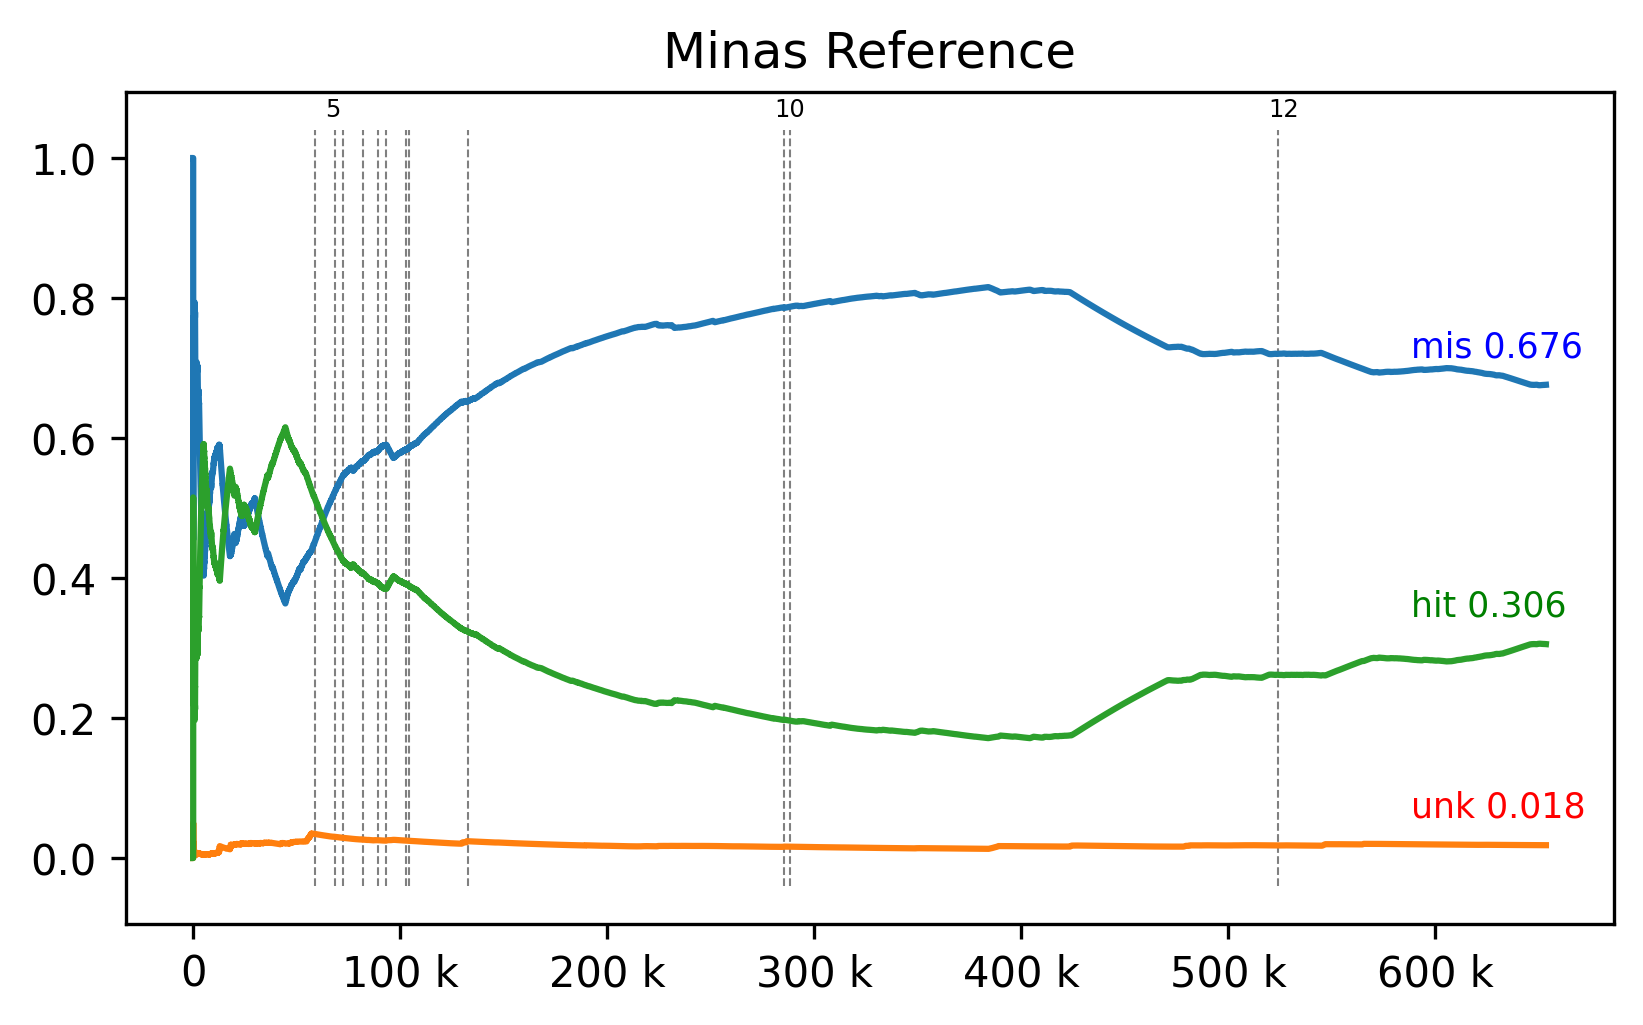
\includegraphics[width=0.75\linewidth]{experiments/revised-java-log.png}
  \caption{Experimento \expA, visualização de fluxo do \dataset \emph{Kyoto} Dez. 2015.}
  \label{fig:validation-java}
\end{figure}

As Figuras \ref{fig:validation-java} e \ref{fig:validation-serial} reforçam a
observação anterior de que mais rótulos novidade (linhas tracejadas verticais
com rótulo no topo) foram encontrados no experimento \expA do que as encontradas 
no experimento \expB.
Outro aspecto com relação a rótulos novidade, no experimento \expA eles surgem
mais ``cedo'' no fluxo, sendo a primeira marcação em $x=58\,967$ contra $x=94\,155$ no
experimento \expB.

\begin{figure}[htb]
  \centering
  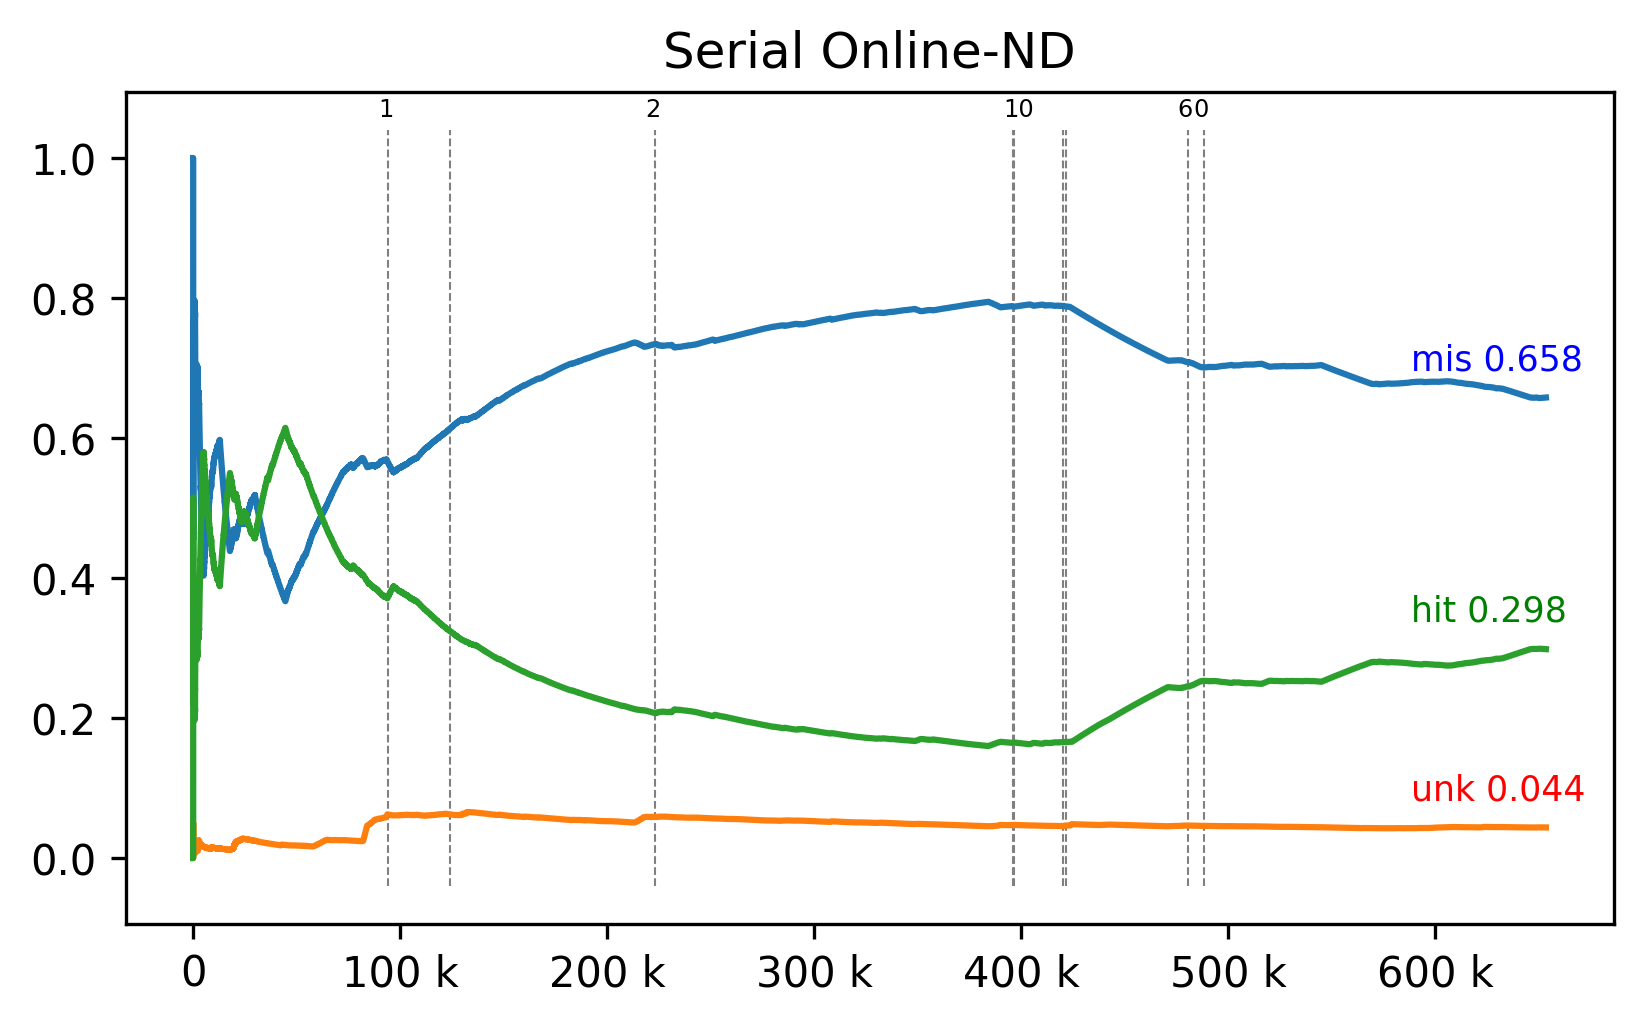
\includegraphics[width=0.75\linewidth]{experiments/online-nd-log.png}
  \caption{Experimento \expB, visualização de fluxo do \dataset \emph{Kyoto} Dez. 2015.}
  \label{fig:validation-serial}
\end{figure}

O gráfico de visualização do fluxo tem no eixo horizontal (x, domínio) o índice
do exemplo $x$ e o eixo vertical (y, imagem) mostra o valor das métricas de qualidade
calculadas até aquele índice de exemplo $x$ no fluxo de saída capturado.
As linhas horizontais na visualização de fluxo mostram o progresso das métricas
de qualidade de classificação durante o fluxo e, ao final na esquerda, o valor
impresso junto e de mesma cor da linha é o valor final de cada métrica.
As métricas são: 
em laranja a taxa de desconhecidos (\texttt{unk}),
em verde a acurácia (\texttt{hit}) e
em azul o erro (\texttt{err}).
Estas métricas podem ser arranjadas em uma tripla-sumário
(\texttt{unk}, \texttt{hit}, \texttt{err})
com os valores em pontos percentuais para fácil comparação.

% Por último, o gráfico de visualização do fluxo mostra as métricas de qualidade
% resumida (\ emph {Acessos}, \ emph {Desconhecidos}, \ emph {Erros}) computada
% para cada exemplo no fluxo de saída capturado. Este resumo é calculado para cada
% exemplo, mas usa a linha \ emph {Atribuída} calculada anteriormente para avaliar
% \ emph {Acertos}; as outras medidas são derivadas conforme descrito antes. 

% Lastly, the stream visualization chart shows the summary quality measurement
% (\emph{Hits}, \emph{Unknowns}, \emph{Misses})
% computed for each example in the captured output stream.
% This summary is computed for each example, but it uses the \emph{Assigned} row
% computed previously to evaluate \emph{Hits}; the other measurements are derived as
% described before.
% The Horizontal axis (x, domain) plots the index of the example and the
% vertical axis (y, image) shows the measurement computed until that example index on the captured
% output stream.

Em conclusão das métricas de qualidade de classificação, os experimentos \expA e
\expB não são idênticos, pois não implementam a mesma definição para o raio,
porém são equivalentes em seus resultados.
Enquanto o experimento \expA tem tripla-sumário
($1.8\%,\: 30.6\%,\: 67.6\%$),
o experimento \expB piora marginalmente nas métricas com
($4.4\%,\: 29.8\%,\: 65.8\%$),
tendo mais desconhecidos, menor acurácia e menor erro.

Para as métricas de escalabilidade, os experimentos \expA e
\expB servem somente como base
para os próximos experimentos onde o paralelismo passa a ser utilizado.
Uma última nota quanto ao tempo de execução, mesmo não sendo paralelo, as
otimizações de memória, redução do uso de \emph{strings} e condição de parada do
algoritmo \emph{K-Means}, reduziram o tempo utilizado pela implementação de
referência de $2\;772s$ ($917s$ \emph{offline} e $1\;845s$ \emph{online}) para
$287s$ ($194s$ \emph{offline} e $93s$ \emph{online} no experimento \expB) na
nova implementação.

\subsection{Paralelismo e Distribuição}
\label{subsec:parallel-dist}

% For the measurements summary table, six measurements from two sources are displayed. Three
  % measures \emph{Hits}, \emph{Unknowns} and \emph{Misses} represented as ratio of
  % the captured output stream, extracted from the evaluation python program,
  % computed as follows:
  % \emph{Hits} (true positive rate) is the sum of the \emph{Hits} row in the
  % extended confusion matrix;
  % \emph{Unknowns} is the count of examples in the captured output stream marked
  % with the \emph{unknown} label (\emph{``-''});
  % \emph{Misses} is the count of all examples in the captured output stream marked
  % with a label distinct from the \emph{Assigned} original class and are not marked
  % as unknown.

  % Furthermore in the measurement summary table, \emph{Time}, \emph{System} and \emph{Elapsed}
  % represented in seconds, are extracted from \emph{GNU Time 1.9}.
  % \emph{Time} is the amount of CPU seconds expended in user-mode
  % (indicates time used doing CPU intensive computing, e.g., math);
  % \emph{System} is the amount of CPU seconds expended in kernel-mode
  % (for our case, it indicates time doing input or output);
  % \emph{Elapsed} is the real-world (wall clock) elapsed time and
  % indicates how long the program took to complete.
  % The lower the times, the better.
  % Our four main experiments are shown in Tab. \ref{tab:exper-summary}.

  % Lastly, the stream visualization chart shows the summary quality measurement
  % (\emph{Hits}, \emph{Unknowns}, \emph{Misses})
  % computed for each example in the captured output stream.
  % This summary is computed for each example, but it uses the \emph{Assigned} row
  % computed previously to evaluate \emph{Hits}; the other measurements are derived as
  % described before.
  % The Horizontal axis (x, domain) plots the index of the example and the
  % vertical axis (y, image) shows the measurement computed until that example index on the captured
  % output stream.

  % Adding to the stream visualization chart, novelty label markers are represented
  % as vertical lines indicating \emph{when} in the captured output stream a new
  % label first appeared.
  % Some of the novelty label markers include the label itself ($l \in \mathbb{N}$)
  % for reference (showing every label would turn this feature unreadable due
  % to overlapping).
  % Figure \ref{fig:visualization} shows complete stream visualization charts.

  % \begin{table*}[htb]
  % \caption{Confusion Matrixes and Qualitative measurements}
  % \label{tab:confusion-matrixes-ref-serial}

% \vspace{3ex}

Seguindo as comparações, para avaliar a escalabilidade dos sistemas, foram
realizados dois experimentos que seguem o mesmo roteiro, o experimento \expC (1 nó e
4 núcleos) e o experimento \expD (3 nós e 12 núcleos).
As Tabelas \ref{tab:single-matrix} e \ref{tab:multi-matrix} mostram as matrizes
de confusão dos experimentos \expC e \expD respectivamente.

\begin{table}[hbt]
  \centering
  % \setlength\tabcolsep{0.5em}
  \caption{Experimento \expC, \mfog com 1 nó e 4 núcleos, Matriz de confusão do \dataset \emph{Kyoto} Dez. 2015.}
  \label{tab:single-matrix}
  \begin{tabular}{l|r|r|r|r|r|r|r}
    Rótulos &      - &       N &    0 &    1 &   2 &  3 &  4 \\\hline
    Classes  &        &         &      &      &     &    &    \\\hline
    \hline
    A        &  12\;282 &  433\;797 &  147 &  952 &   0 &  0 &  1 \\\hline
    N        &   3\;088 &  203\;019 &   40 &   99 &  27 &  5 &  0 \\\hline
    \hline
    Associação &      - &       N &    A &    A &   N &  N &  A \\\hline
    Hits ($tp$)     &      0 &  203\;019 &  147 &  952 &  27 &  5 &  1 
  \end{tabular}
\end{table}

A tripla-sumário do experimento \expC é ($2.4\%,\: 31.2\%,\: 66.4\%$), com menos
desconhecidos em relação ao experimento \expB ($4.4\%,\: 29.8\%,\: 65.8\%$).
A redução de desconhecidos é de $2\%$, sendo distribuída $1.4\%$ em acurácia e
$0.6\%$ em erro, representando melhora marginal em todas as métricas.

% há algo estranho nesta frase, parece que falta uma vírgula ou conjunção...

Comparando as matrizes dos experimentos \expB e \expC, observa-se os
efeitos do paralelismo de classificadores e, mais importante, a execução
assíncrona da tarefa de detecção de novidade.
O impacto principal é a redução no número de rótulos novidade, de $9$ para $5$.
Comparando a visualização de fluxo, Figuras \ref{fig:validation-serial} e
\ref{fig:single-flow}, observa-se também que a aparição do primeiro padrão
novidade acontece mais ``tarde''; enquanto em \expB o rótulo novidade ``1'' é
observado em $x = 94\:155$, em \expC o mesmo rótulo é observado em $x =
172\:917$.

Esse comportamento é devido à detecção de novidade assíncrona, pois enquanto
essa tarefa é executada os classificadores continuam utilizando o modelo antigo.
Além disso, como já foi elencado na Seção \ref{sec:polices} item
\ref{reclassification}, os exemplos utilizados para formar o novo \mcluster
com rótulo novidade não são recolocados no fluxo de saída para nova análise.
Estas duas características do \mfog acarretam em um atraso significativo entre a
aparição de um padrão no fluxo de entrada e a aparição do rótulo correspondente
no fluxo de saída.
Em outras palavras, o fluxo avança com o modelo antigo e, mesmo após atualizado,
só gera uma saída com o rótulo novo quando (e se) o padrão aparece novamente.
Este é um resultado muito importante para compreender os problemas relacionados
à distribuição de um algoritmo deste gênero.

\begin{table}[hbt]
  \centering
  % \setlength\tabcolsep{0.5em}
  \caption{Experimento \expD, \mfog com 3 nós de 4 núcleos cada, Matriz de confusão do \dataset \emph{Kyoto} Dez. 2015.}
  \label{tab:multi-matrix}
  \begin{tabular}{l|r|r|r|r|r|r|r}
    Rótulos   &      - &       N &    0 &    1 &    2 &    3 &  4 \\\hline
    Classes   &        &         &      &      &      &      &    \\\hline
    \hline
    A      &  12\;378 &  433\;631 &  117 &  886 &    0 &  162 &  5 \\\hline
    N      &   3\;121 &  202\;916 &   40 &   96 &  105 &    0 &  0 \\\hline
    \hline
    Associação   &      - &       N &    A &    A &    N &    A &  A \\\hline
    Hits ($tp$)   &      0 &  202\;916 &  117 &  886 &  105 &  162 &  5 
  \end{tabular}
\end{table}

Avançando para o experimento \expD, a matriz de confusão na Tabela
\ref{tab:multi-matrix}, mostra pouca diferença quando comparado ao experimento
\expC, com o número de desconhecidos sofrendo a maior variação.

O mesmo é observado quando compara-se a visualização de fluxo, Figuras
\ref{fig:single-flow} e \ref{fig:multi-flow}, há pouca diferença e a tripla-sumário
($2.4\%,\: 31.2\%,\: 66.4\%$) é idêntica.

\begin{figure}[htb]
  \centering
  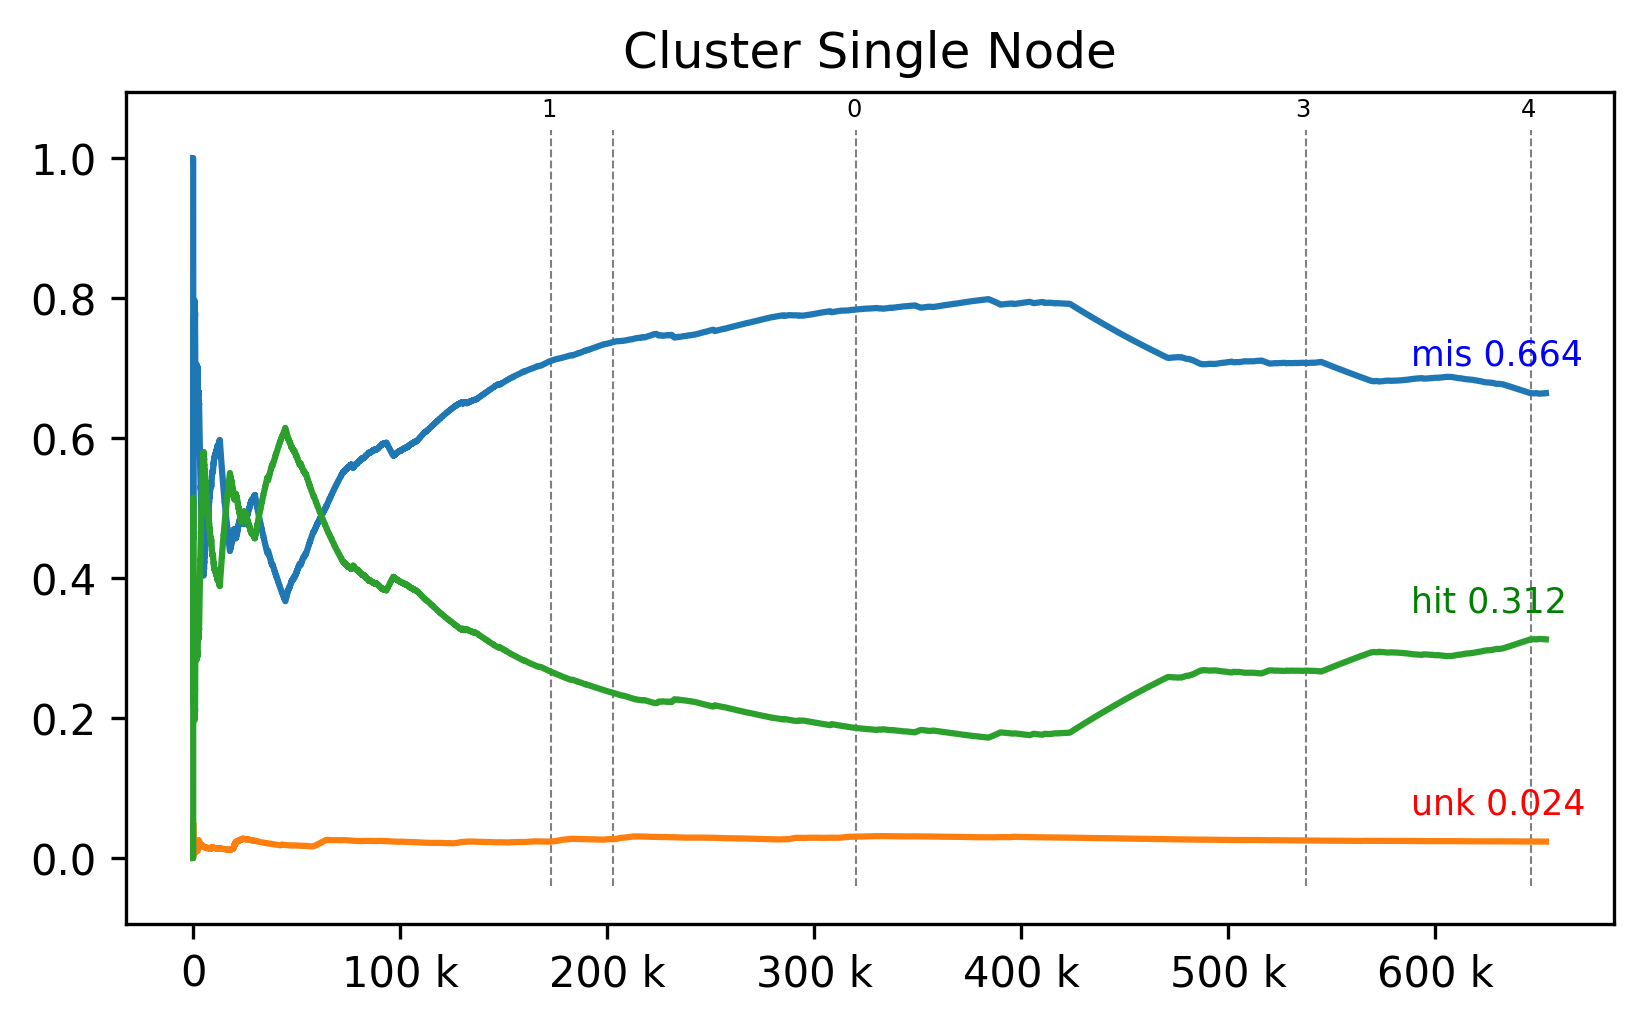
\includegraphics[width=0.75\linewidth]{experiments/tmi-base-log.png}
  \caption{Experimento \expC, \mfog com 1 nó e 4 núcleos, visualização de fluxo do \dataset \emph{Kyoto} Dez. 2015.}
  \label{fig:single-flow}
\end{figure}

\begin{figure}[htb]
  \centering
  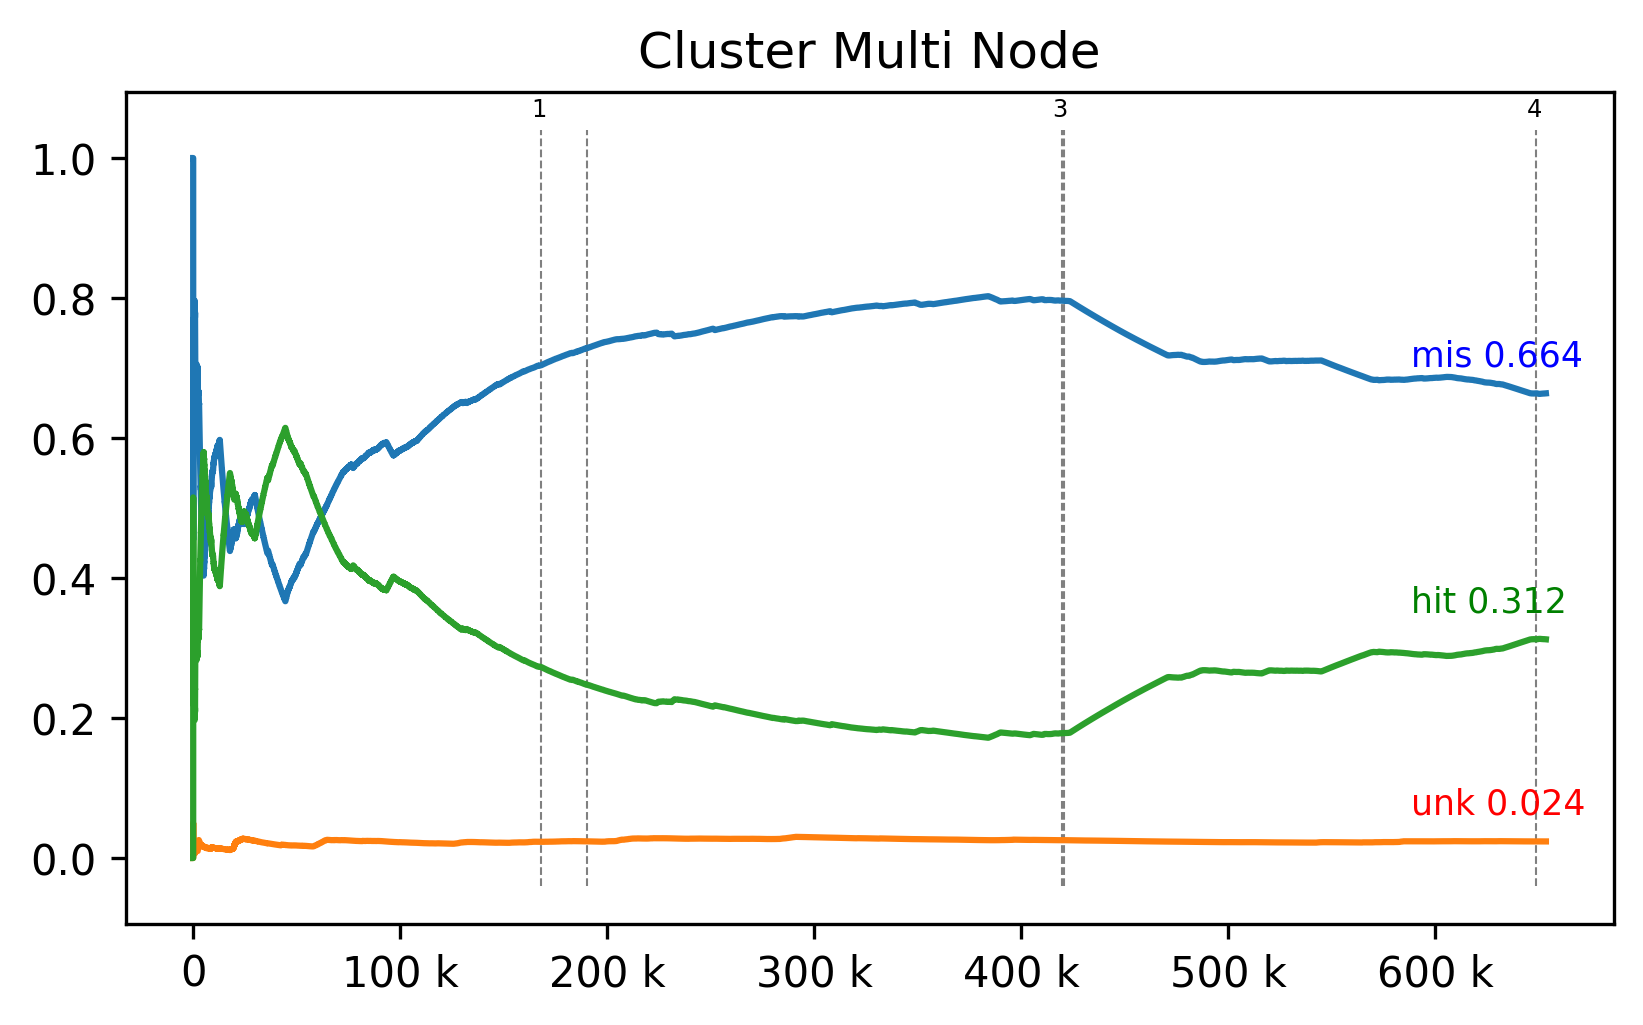
\includegraphics[width=0.75\linewidth]{experiments/tmi-n12-log.png}
  \caption{Experimento \expD, \mfog com 3 nós de 4 núcleos cada, visualização de fluxo do \dataset \emph{Kyoto} Dez. 2015.}
  \label{fig:multi-flow}
\end{figure}

Isto reforça a ideia de que o maior impacto nas métricas de qualidade de
classificação é a mudança de detecção de novidade assíncrona, pois mesmo com o
triplo de instâncias classificadoras, as métricas continuam idênticas.

Com a discussão das métricas de qualidade de classificação concluída, resta
abordar as métricas de escalabilidade que são muito mais simples em sua
definição e extração porém de muito interesse a este trabalho.

Essas métricas de escalabilidade extraídas dos experimentos são número de núcleos de processamento
utilizados, \emph{Tempo}, \emph{Sistema} e \emph{Decorrido}, representados em
segundos, e obtidas via \emph{GNU Time 1.9} durante a execução do experimento
em questão.
\emph{Tempo} é a quantidade de segundos de CPU gastos no modo de usuário
(indica o tempo usado em computação intensiva, por exemplo cálculos matemáticos).
\emph{Sistema} é a quantidade de segundos de CPU gastos no modo \emph{kernel} (para
nosso caso, indica o tempo de entrada ou saída).
\emph{Decorrido} é o tempo decorrido do mundo real (relógio de parede) e indica
quanto tempo o programa levou para ser concluído.
Quanto mais baixos os tempos, melhor.

Os quatro experimentos principais são mostrados na Tabela
\ref{tab:exper-summary}, relacionando as métricas de qualidade de classificação
da tripla-sumário (\texttt{unk}, \texttt{hit}, \texttt{err}) e as métricas de
escalabilidade.

Na Tabela \ref{tab:exper-summary}, a coluna \emph{Offline} representa os valores
de métricas de tempo de execução para a fase \emph{Offline} (treinamento) nos
experimentos utilizando o \mfog (\expB, \expC e \expD).
Esta distinção é necessária pois a implementação de referência do algoritmo
\minas executa as duas fases sem separação. Já o tempo de treinamento no \mfog é
mostrado na coluna \emph{Offline}.
Uma modificação da implementação de referência mostrou que dos $2\;772.07$
segundos listados na tabela, $917s$ são da fase \emph{offline} e $1\;845s$ da
fase \emph{online}.

\newcommand{\mr}[1]{\multirow{2}{*}{\texttt{#1}}}

\begin{table}[hbt]
  \centering
% \setlength\tabcolsep{0.35em}
\setlength\extrarowheight{2pt}
  \caption{Sumário das métricas extraídas dos experimentos principais.}
  \label{tab:exper-summary}
  \begin{tabular}{l|r|r|r|r|r}
  Experimento     & \expA         & \emph{Offline} & \expB     & \expC    & \expD    \\
  Métrica         &               &               &                 &                 &        \\\hline
  \mr{unk}        & $11980$       &               & $28567$         & $15370$     & $15499$     \\
                  & $0.018333$    &               & $0.043717$      & $0.023521$  & $0.023718$  \\\hline
  \mr{hit}        & $199708$      &               & $195017$        & $204151$    & $204191$    \\
                  & $0.305618$    &               & $0.298438$      & $0.312416$  & $0.312478$  \\\hline
  \mr{err}        & $441769$      &               & $429873$        & $433936$    & $433767$    \\
                  & $0.676049$    &               & $0.657843$      & $0.664061$  & $0.663802$  \\\hline
  Tempo     ($s$) & $2761.83$     & $194.12$      & $80.79000$      & $522.1000$  & $207.1400$  \\\hline
  Sistema   ($s$) & $7.15$        & $ 0.075$      & $11.51000$      & $ 47.7700$  & $157.6100$  \\\hline
  Decorrido ($s$) & $2772.07$     & $194.27$      & $93.03000$      & $145.0400$  & $ 95.3800$  \\\hline
  Latência  ($s$) & $4.24\cdot10^{-3}$  &       & $1.42\cdot10^{-4}$  & $2.22\cdot10^{-4}$  & $1.46\cdot10^{-4}\ $  \\\hline
  Processadores   & $1$           &  $1$          &  $1$            & $4$         & $12$        \\\hline
  \emph{Speedup}  &               &               &                 & $0.6414092$ & $0.9753617$  \\\hline
  Eficiência      &               &               &                 & $0.1603523$ & $0.0812801$  
  \end{tabular}
\end{table}

Além das métricas extraídas dos experimentos, as métricas de escalabilidade
calculadas a partir dos valores extraídos são a latência de eventos e
\emph{speedup}. % prático.
A latência média é calculada com o tempo decorrido dividido pelo o tamanho do
\dataset e pode ser vista na Tabela \ref{tab:exper-summary}.
O \emph{speedup} é calculado com a divisão do tempo decorrido na versão
sequencial divido pelo tempo utilizado pela versão paralela.
A eficiência é calculada com a divisão do tempo decorrido na versão sequencial
divido pelo produto do número de processadores utilizado e o tempo utilizado
pela versão paralela.

Observando as métricas de escalabilidade nota-se que o \mfog não fornece
\emph{speedup} e eficiência em relação à versão sequencial.
Isto indica que, apesar da premissa de independência de classificadores
paralelos, a comunicação entre os processos utilizando dois conjuntos de
instruções \mpi \emph{send} e \emph{receive} para cada exemplo não é eficiente
para o processamento de fluxo de dados.

\subsection{Experimentos Adicionais}

Experimentos adicionais foram realizados para avaliar o comportamento do \mfog
para número variado de processadores entre $1$ e $12$ utilizando de $1$ a $3$ nós.
Os resultados obtidos, ilustrados na Figura \ref{fig:speedup}, são limitados ao
nó raiz, e mostram um aumento do tempo \emph{Sistema} (operações em modo
\emph{kernel}).
Este aumento indica maior carga associada às operações de entrada e saída das
instruções \emph{send} e \emph{receive} reforçando a ideia apresentada na
Subseção \ref{subsec:parallel-dist}.

Outros experimentos adicionais foram realizados para averiguar a latência para
cada exemplo do fluxo, mostrando o comportamento de cada implementação, o que é
ilustrado nas Figuras \ref{fig:lag-java}, \ref{fig:lag-serial} e
\ref{fig:lag-mfog}.
No entanto, é importante destacar que esta métrica não foi extraída dos
experimentos principais, sendo apenas ilustrativa dos diferentes comportamentos.

% não entendi essa questão de que os dados não foram obtidos de experimentos. Como os gerou?

O primeiro comportamento é ilustrado na Figura \ref{fig:lag-java}, onde a execução
da tarefa de detecção de novidade gera picos de $50$ a $200$ segundos.
Um comportamento semelhante é visto na Figura \ref{fig:lag-serial} onde ainda há
picos de latência, porém não tão intensos e frequentes.
Esta diferença está relacionada com mecanismo de remoção de desconhecidos e
ausência do mecanismo de esquecimento de \mclusters menos utilizados no Modelo.
Já o comportamento visto na Figura \ref{fig:lag-mfog} mostra o efeito de
\emph{buffers} de comunicação entre diferentes processos onde o pico de latência
da detecção de novidade cai progressivamente conforme os buffers são esvaziados
já que o processo de detecção de novidade é assíncrono, porém ocupa a \emph{thread}
responsável pelo fluxo de saída do \mfog.

\begin{figure}[htb]
  \centering
  \begin{minipage}{0.49\textwidth}
    \centering
    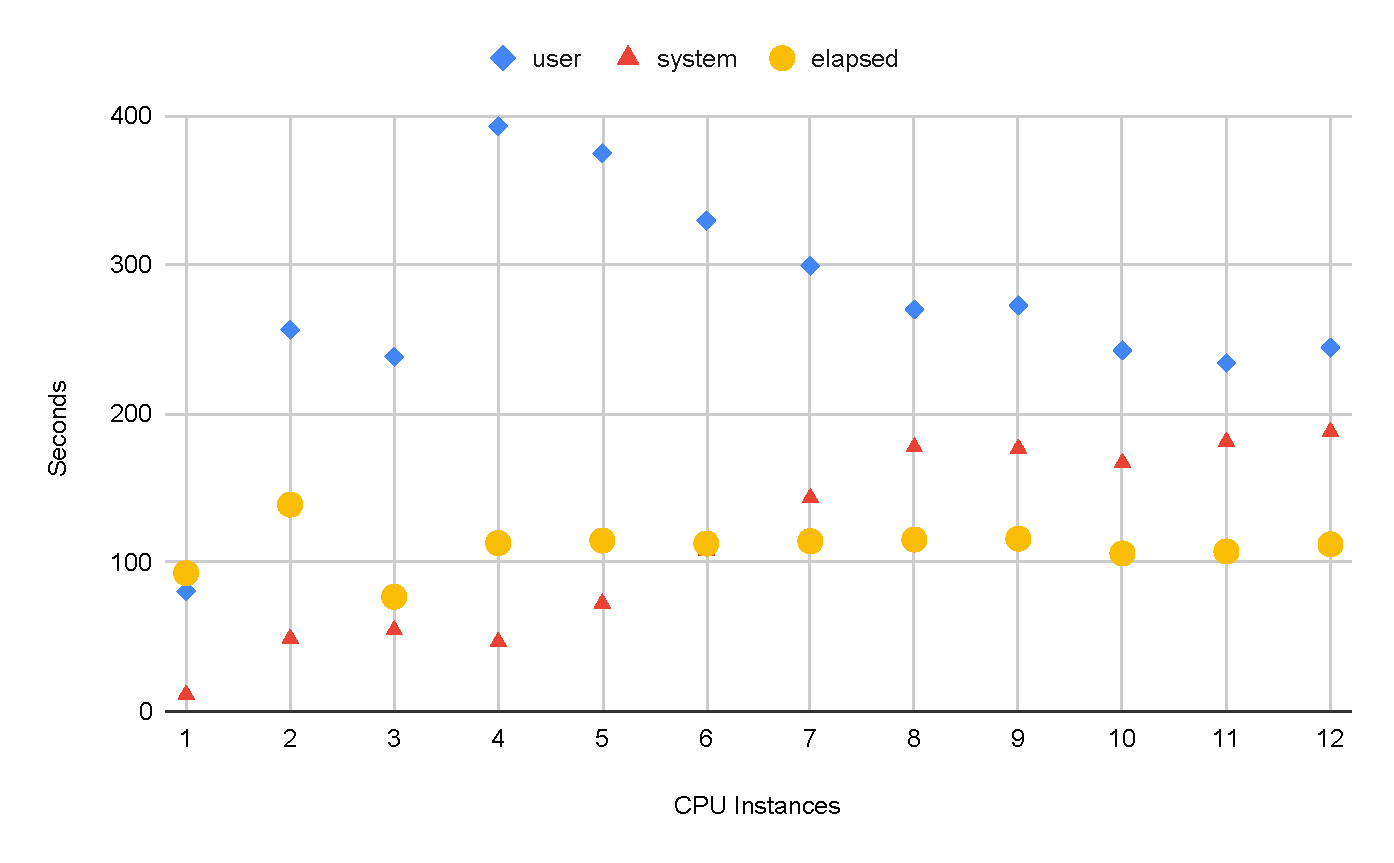
\includegraphics[width=1\linewidth,page=1]{experiments/speedup-clean.pdf}
    \caption{Métricas de tempo para execuções do \mfog com variação no número de processadores.}
    \label{fig:speedup}
  \end{minipage}
  \hfill
  \begin{minipage}{0.49\textwidth}
    \centering
    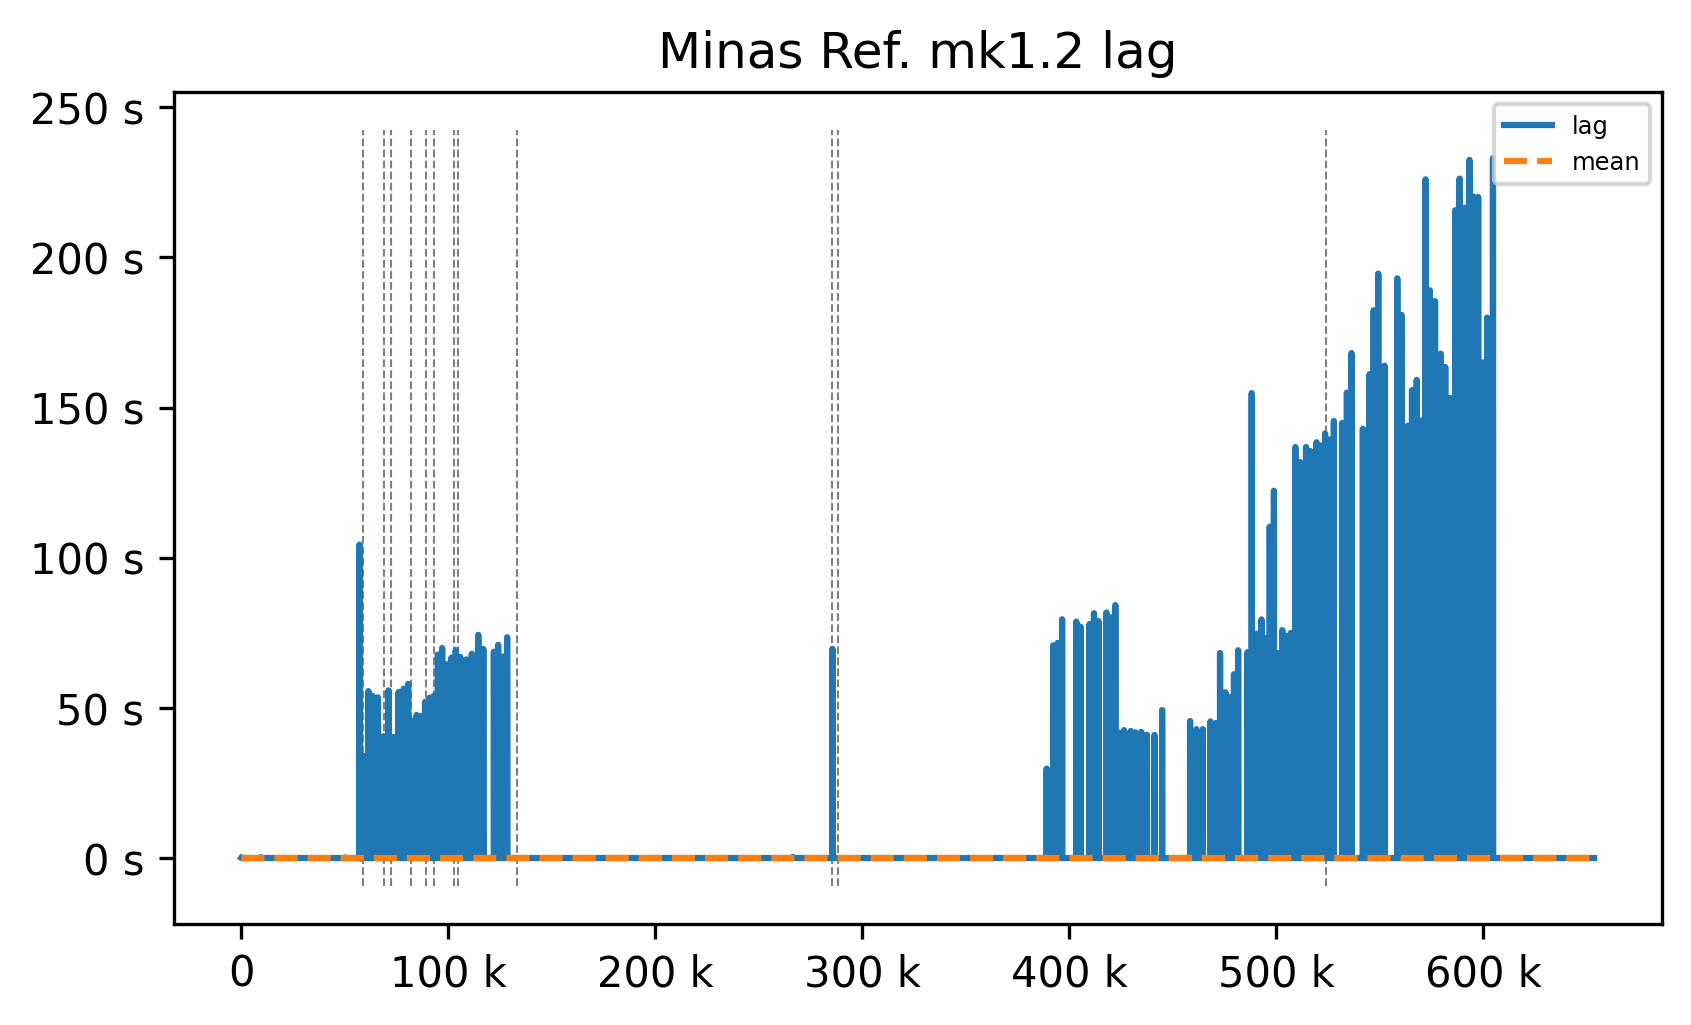
\includegraphics[width=1\linewidth]{experiments/lag-java.png}
    \caption{Visualização de Latência, Implementação de referência do algoritmo \minas.}
    \label{fig:lag-java}
  \end{minipage}
  % \hfill
  \vspace{5mm}
  \begin{minipage}{0.49\textwidth}
    \centering
    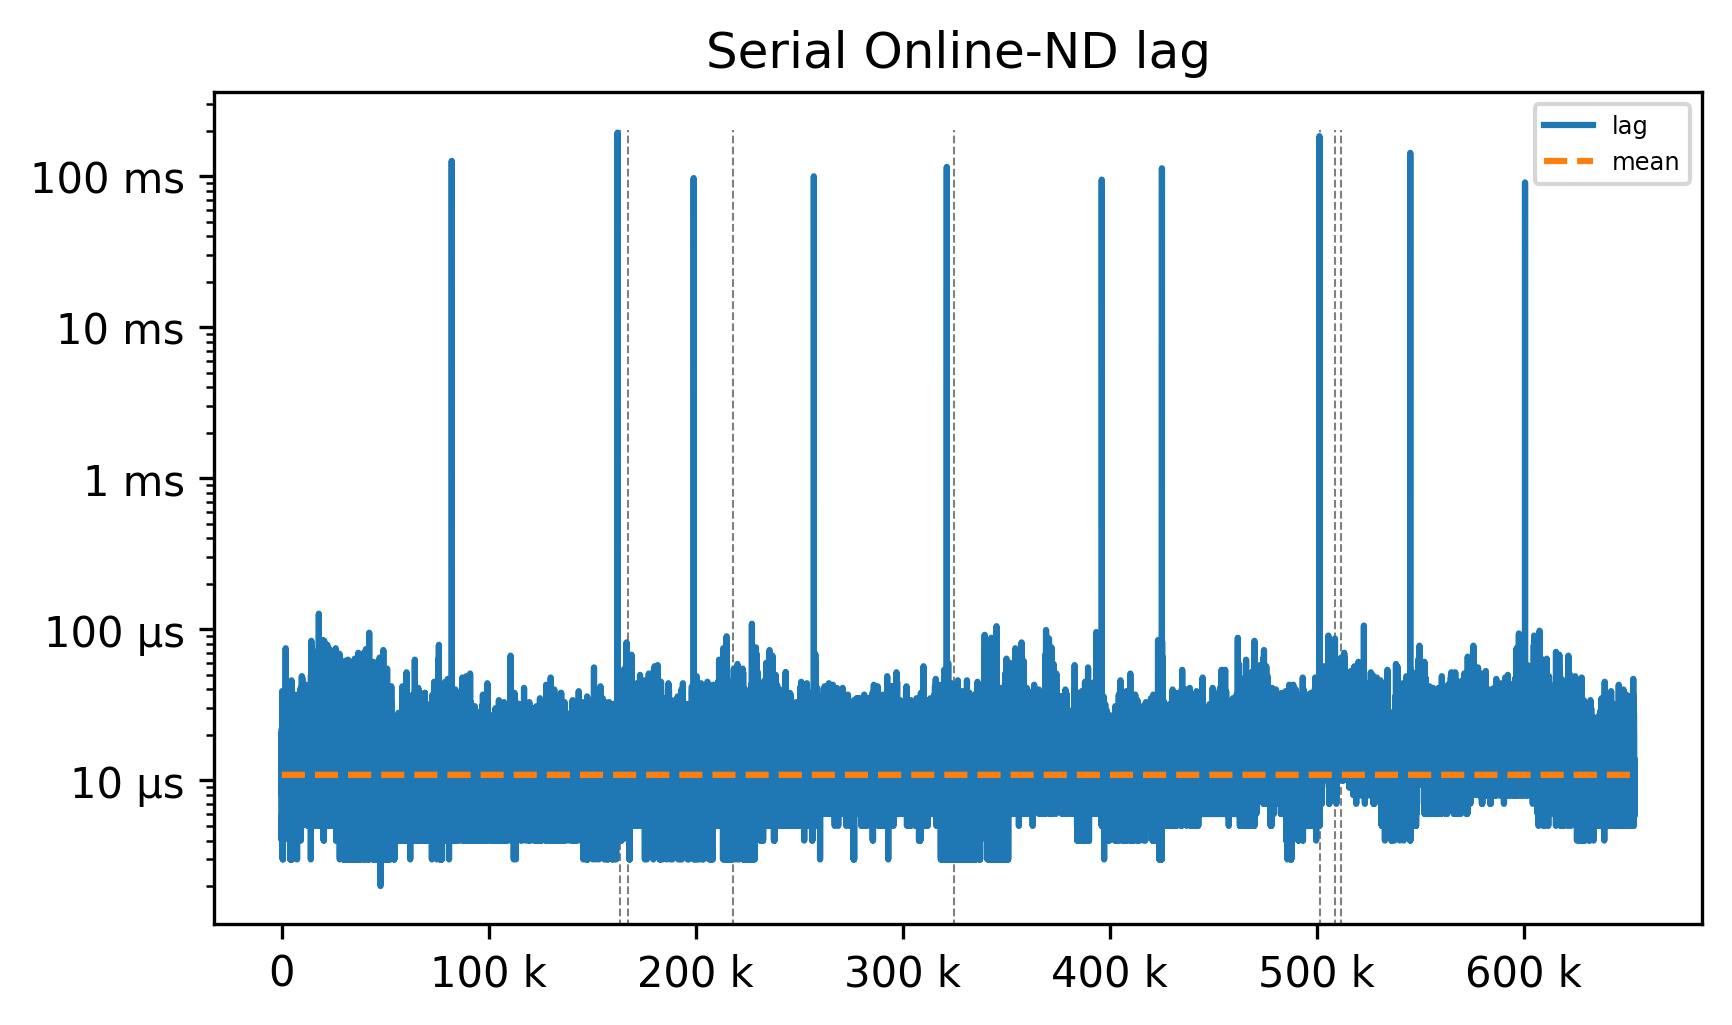
\includegraphics[width=1\linewidth]{experiments/lag-serial.png}
    \caption{Visualização de Latência na Implementação \emph{Serial} do algoritmo \minas usando funções do \mfog.}
    \label{fig:lag-serial}
  \end{minipage}
  % \vspace{5mm}
  \hfill
  \begin{minipage}{0.49\textwidth}
    \centering
    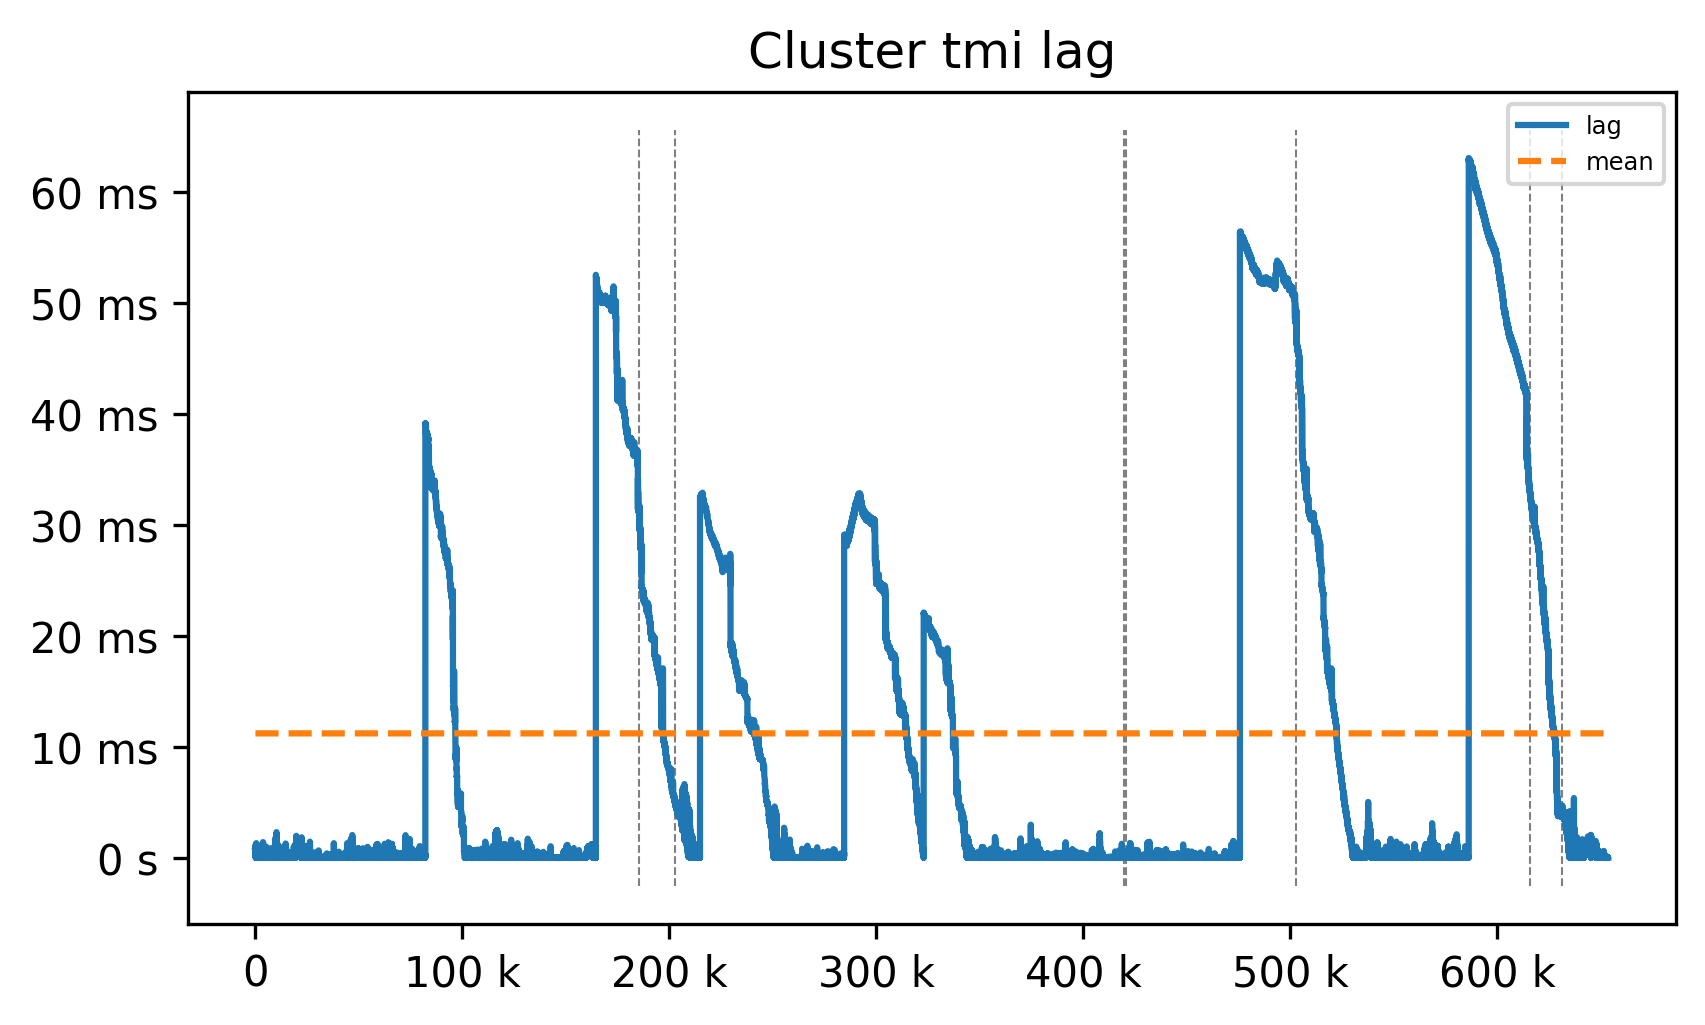
\includegraphics[width=1\linewidth]{experiments/lag-mfog.png}
    \caption{Visualização de Latência no \mfog.}
    \label{fig:lag-mfog}
  \end{minipage}
  % \caption{Experimentos adicionais \dataset \emph{Kyoto} Dez. 2015. Experimento fora do ambiente de \fog.}
  % \label{fig:lag}
\end{figure}

\FloatBarrier
\section{Conclusão}
\label{sec:exp-conclusao}

Os experimentos executados e os resultados obtidos demonstram que a
\acf{ND-DS} executada de maneira distribuída em ambiente de névoa (\fog) é
viável como  parte de um \acf{NIDS} para redes \iot.\todo[inline]{Poderia dizer que se mostrou uma estratégia válida para detecção de mudanças nos padrões de tráfego.}


No entanto para aplicação em uma situação real, são necessárias otimizações
desde o \dataset de treinamento e avaliação, passando pelo algoritmo de detecção
de novidade, parâmetros do algoritmo e estratégias de paralelismo e
distribuição.

% !TeX root = ./00.ppgcc-2020.tex

\chapter{Conclusão}\label{cha:final}

% \begin{resumocap}
%   Este Capítulo resume o trabalho realizado até agora e estabelece
%   os próximos passos até sua completude.
% \end{resumocap}

% retomar motivacao aqui
Segurança e privacidade são uma grande preocupação em \acf{IoT}, seja para a
preservação do sigilo de dados pessoais ou para evitar a subversão do
dispositivo para uso em uma \emph{botnet}. Nesses  cenários,
o monitoramento da rede para detecção
de possíveis intrusões é uma tarefa necessária.
Atendendo a essa necessidade, um \acf{NIDS} é uma ferramenta que observa o
tráfego da rede e alerta para possíveis ataques.
Este alerta pode ser gerado através de detecção de anomalias, e uma técnica para
detectar anomalias são algoritmos de \acf{ND}. O algoritmo \minas é um
algoritmo de detecção de novidade que já foi avaliado e considerado promissor para aplicação em \nids.

Para um bom funcionamento de um \nids, é necessário que este responda rapidamente
aos padrões do fluxo da rede. Portanto, para aplicações em redes \iot o envio das
observações de uma rede remota para processamento em nuvem pode resultar em latências proibitivas. 
Uma alternativa viável à computação em nuvem neste caso é a computação em névoa
que pode disponibilizar recursos computacionais mais próximos
à fonte de dados, mesmo que de menor capacidade, oferece menor latência em seus processamentos.
Porém, a necessidade de resposta rápida de um \nids e a natureza distribuída da
computação em névoa requer que as técnicas utilizadas estejam preparadas para
um cenário paralelo e distribuído, o que não acontece com o algoritmo \minas.

% cumpriu objetivo 1?? - propõem-se a construção de uma aplicação que implemente o
% algoritmo MINAS (FARIA; CARVALHO; GAMA, 2016) de maneira escalável e distribuível
% para ambientes de computação em névoa, seguindo a arquitetura
Este trabalho apresenta a construção e avaliação do \mfog, uma implementação
paralela e distribuída com foco na execução em névoa de dispositivos \iot do
algoritmo \minas, pautado em um caso de uso para \nids seguindo a arquitetura \arch \cite{Cassales2019a}.
Esta implementação foi construída com \mpi buscando a escalabilidade na tarefa de
processamento de fluxo de dados e economia dos recursos limitados comumente
encontrados em sistemas \iot.

% cumpriu obj 2 ??- Além disso, propõem-se também a avaliação dessa implementação
% com experimentos baseados na literatura usando conjunto de dados públicos
% relevantes.
A avaliação do sistema construído utilizou o conjunto de dados (\dataset)
\emph{Kyoto 2015}, relevante para \nids por conter descritores de fluxo de uma
rede de \emph{Honeypots}.
A manipulação do conjunto de dados utilizado, apesar de não otimizada, foi
suficiente para avaliar a implementação e comparar resultados.

% cumpriu obj? - implemen-tar o algoritmo MINAS de maneira distribuída sobre uma
% plataforma de processamento distribuída de fluxos de dados

% cumpriu obj?? - Arquitetar e implementar um mecanismo de execução e avaliação de
% qualidade e desempenho para os ambientes escolhidos
As métricas de qualidade de classificação escolhidas mostraram resultado
equivalente entre a nova implementação e a implementação de referência do
algoritmo \minas, seja na versão sequencial, paralela com 4 processadores ou
distribuída com 3 nós.
As métricas de escalabilidade do \mfog em ambiente de névoa \iot mostraram
melhora significante comparada à implementação de referência no mesmo ambiente.
\notake{pq?}
\hlke{No entanto não foi observada melhora compatível com o aumento no número de nós
no cluster} (eficiência da computação paralela), ou seja, a escalabilidade
almejada não foi alcançada.
% cumpriu?? Avaliar e comparar a qualidade de detecção de intrusão da nova
% implementação;

As principais contribuições deste trabalho são a análise, implementação revisada
e melhora do desempenho do algoritmo \minas guiado pelo contexto de computação
distribuída em névoa de dispositivos \iot e, adição de uma técnica palpável para
\nids, contribuindo para redução de danos a quem depende do bom funcionamento
dos sistemas em redes \iot.

% cumpriu?? - Avaliar a qualidade de detec-ção de intrusão em ambiente distribuído
% conforme a arquitetura IDSA-IoT em ambientede computação em névoa.

% se cumptri objetivo como cumpriu e qual foi o resultado????

% chegou-se ao resultao esoerado? - O resultado esperadoé uma implementação
% compatível em qualidade de classificação ao algoritmo MINAS epassível de ser
% distribuída em um ambiente de computação em névoa aplicado à detecçãode
% intrusão.


% qual a conclusao geeral sobre sua ilmplementacao? ta distribuida? é escalave? eh
% comparavel com estado da arte pra pior/melhor/igual?
Para o problema \nids em redes \iot (ou detecção de comportamentos anômalos em
fluxos de dados de sensores \iot em geral) com base em \nd paralela e
distribuída em névoa, o equilíbrio dos atributos de escalabilidade e
qualidade de classificação ainda não foi alcançado.

Para trabalhos futuros, espera-se que esta implementação e análise sirva de
inspiração para busca de algoritmos e sistemas que maximizam o aproveitamento do
\emph{hardware} e energia dedicados a esta tarefa.
% o que vc  poderia melhorar/??
Em termos mais práticos, sugere-se a utilização do algoritmo \emph{CluStream}
\cite{Aggarwal2003} ou seus derivados e a ideia de um Modelo de tamanho fixo,
maximizando o aproveitamento de memória e a acurácia com um grande conjunto de
\mclusters.
Seguindo esta sugestão, estes \mclusters podem ser definidos como polígonos para
melhor cobertura do espaço, o Modelo pode ser checado quanto à sobreposição
evitando ambiguidade e o Modelo organizado em índices para que a busca espacial
seja rápida e eficiente.
Acredita-se que estas características junto com as propriedades de paralelismo e
distribuição em névoa podem levar a resultados brilhantes.

% -------------------------------------------------------------

% Este trabalho reúne conceitos de aprendizado de máquina com ênfase em detecção
% de novidades em fluxos contínuos de dados e conceitos de processamento
% distribuído de fluxos contínuos, com o objetivo de unir a lacuna no estado da
% arte desses conceitos à luz de uma implementação e avaliação no cenário de
% detecção de intrusão em redes de dispositivos da Internet das Coisas (\iot) em
% ambiente de computação em névoa (\fog).

% O objeto central desse trabalho (\mfog) trata da implementação do algoritmo MINAS na
% plataforma de processamento de fluxos \flink, em três módulos que podem ser
% distribuídos em um ambiente de \fog.
% Sua distribuição permite selecionar o nó que tem os recursos computacionais mais
% adequados para cada tarefa.
% A avaliação do \mfog será feita por
% meio de métricas de qualidade
% de classificação e métricas de escalabilidade.

% Dando continuidade a este trabalho, segue-se com o desenvolvimento da implementação objeto
% (\mfog) bem como a contínua avaliação comparativa dos resultados
% produzidos pelo \mfog com seu algoritmo base, MINAS.
% Também será dada continuidade nos experimentos com os conjuntos de dados (\datasets)
% diversos e configurações variadas de distribuição de processamento em \fog
% extraindo desses experimentos as métricas previamente discutidas.

% Dessa forma, o \mfog pode contribuir com adição de uma ferramenta para os interessados
% em sistemas de detecção de intrusão de redes de dispositivos \iot
% ou outros sistemas que tratam de fluxos contínuos que tradicionalmente sofrem
% com os ônus de latência e largura de banda na comunicação entre borda e nuvem.
% Além disso, o \mfog objetiva contribuir com a adição de uma implementação
% distribuída de um algoritmo cujo modelo é estado da arte em detecção de
% novidades em fluxos contínuos de dados.

% \subsection{Conclusion}
% \label{sec:conclusion}

% % A \acf{ND-DS} pode ser um mecanismo útil para \acf{NIDS} em ambientes \acf{IoT}.
% % \nd em ambientes \iot também pode servir a outras tipos de monitoramento
% % contínuo, análisando do comportamento do sistema.
% % Com relação à enorme quantidade de dados que devem ser processados na análise de
% % fluxo para \nd, é melhor que esse processamento ocorra próximo da fonte desses
% % dados, evitando tráfego e latência na comunicação com a nuvem.
% % No entanto, outra característica de redes \iot é a capacidade de processamento
% % reduzida de tais dispositivos de borda.

% Data Stream Novelty Detection (\nd) can be a useful mechanism for Network
% Intrusion Detection (\nids) in IoT environments.
% It can also serve other related applications of \nd using continuous network or
% system behavior monitoring and analysis.
% Regarding the tremendous amount of data that must be processed in the flow
% analysis for \nd, it is relevant that this processing takes place at the edge of
% the network.
% However, one relevant shortcoming of the IoT, in this case, is the reduced
% processing capacity of such edge devices.

% In this sense, we have put together and evaluated a distributed architecture for
% performing \nd in network flows at the edge.
% Our proposal, \mfog is a distributed \nd implementation based on the \nd
% algorithm \minas.

% The main goal of this work is to observe the effects of our approach to a
% previously serial only algorithm, especially in regards to time and quality
% metrics.

% While there is some impact on the predictive metrics, this is not reflected on
% overall classification quality metrics indicating that distribution of \minas
% shows a negligible loss of accuracy.
% In regards to time and scale, our distributed executions was faster than the
% previous sequential implementation of \minas, but efficient data distribution
% was not achieved as the observed time with each added node remained constant.

% Overall, \mfog and the idea of using distributed flow classification and novelty
% detection while minimizing memory usage to fit in smaller devices at the edge of
% the network is a viable and promising solution.
% Further work include the investigation of other \nd algorithms, other clustering
% algorithms in \minas and analysis of varying load balancing strategies.


% \chapter{Capítulo genérico}
% \lipsum[1]
% \section{Seção genérica}
% \lipsum[3]

% Finaliza a parte no bookmark do PDF, para que se inicie o bookmark na raiz
\bookmarksetup{startatroot}

% ----------------------------------------------------------
% Conclusão
% \chapter*[Conclusão]{Conclusão}
% \addcontentsline{toc}{chapter}{Conclusão}

% \lipsum[31-33]

% ----------------------------------------------------------
% ELEMENTOS PÓS-TEXTUAIS
\postextual

% ----------------------------------------------------------
% Referências bibliográficas
\bibliography{99.referencias.bib}

% ----------------------------------------------------------
% Glossário
%\glossary

% ----------------------------------------------------------
% Apêndices
% Inicia os apêndices
% \begin{apendicesenv}
%    % Imprime uma página indicando o início dos apêndices
%    \partapendices
%    % ----------------------------------------------------------
%    % Incluir Apêndice
%    % ----------------------------------------------------------
%    \chapter{Quisque libero justo}
%    \lipsum[3]
% \end{apendicesenv}

% ----------------------------------------------------------
% Anexos
% \begin{anexosenv}
%    % Imprime uma página indicando o início dos anexos
%    \partanexos
%    \chapter{Morbi ultrices rutrum lorem.}
%    \lipsum[3]
%    \section{Test}
%    \lipsum[3]
% \end{anexosenv}

\end{document}
